% \documentclass[upright, contnum]{umemoria}
\documentclass[upright, contnum]{umemoriaENG}

\usepackage{graphicx}
\usepackage{amsmath}
\usepackage{cancel}
\usepackage{ulem}
% Otros paquetes y configuraciones que quieras agregar

% comandos para comentarios
\newcommand{\redline}{\color{red}\noindent}
\newcommand{\cambiarlinea}[1]{\noindent\textcolor{red}{(cambiar -->) #1}}
\newcommand{\noteEL}[1]{\noindent\textcolor{purple}{(comment-el: #1)}}
\newcommand{\noteTC}[1]{\noindent\textcolor{magenta}{(comment-el: #1)}}
% purple, orange, cyan


% % -- preamble procurement paper
% % \input{preamble-procurement-paper.tex}

% % preamble-procurement-paper
% \def\NN{\mathbb{N}}
% \def\ZZ{\mathbb{Z}}
% \def\PP{\mathbb{P}}
% \def\QQ{\mathbb{Q}}
% \def\RR{\mathbb{R}}
% \def\CC{\mathbb{C}}
% \def\EE{\mathbb{E}}
% \def \rr{ {I\!\!R}}
% \def\cc{{\cal{C}}}
% \def\dis{\displaystyle}
% \def\Var{\text{Var}}
% \def\o{\sigma}


\usepackage[utf8]{inputenc}
\usepackage{amsfonts,setspace}
\usepackage{threeparttable}
\usepackage{dsfont}
\usepackage{color}
\usepackage[dvipsnames]{xcolor}
\usepackage{amssymb}
\usepackage{anysize} %para marginsize%
\usepackage{multicol}
\usepackage{graphicx}
\usepackage{float}
\usepackage{amsmath}
\usepackage{enumerate}
\usepackage{rotating}
\usepackage{comment}
\newcommand{\tblue}[1]{\textcolor{blue}{#1}}
\usepackage{fancyhdr}
\usepackage{color,soul}
\usepackage{lscape}
\usepackage{booktabs, caption, makecell}
\usepackage[format=hang,font=small,labelfont=bf]{caption}
\usepackage{natbib} 
% \usepackage[numbers]{natbib} % Para citas numéricas
% \usepackage[author]{natbib} % Para citas estilo autor-año
\usepackage{authblk}
\usepackage{setspace}
\usepackage{ulem}

\usepackage{hyperref}
 \hypersetup{
     colorlinks=true,
     linkcolor=blue,
     filecolor=blue,
     citecolor = black,      
     urlcolor=cyan,
     }
\hypersetup{linkcolor=black}

\usepackage{multirow}
\usepackage{xcolor}
\usepackage{makecell}
\usepackage{lipsum}


% for marking changes and notes
\usepackage{xcolor, soul}

% Uncomment next line to remove comments
%\def\nocomments{1}
%%%%%%%%%%%%%%%%%%%%%%%%%%%%%%%%%%%%%%%%

% \newcommand{\dani}[1]{{\color{red}[D: #1 ]}}
% \newcommand{\ds}[1]{{\color{red}[D: #1 ]}}

% \newcommand{\piero}[1]{{\color{red}[P: #1 ]}}

% %\setlength{\parskip}{0.5cm}
% \newcommand{\newgw}[1]{\noindent \textcolor{blue}{#1}}
% \newcommand{\delgw}[1]{{\color{blue} \sout{#1}}}
% \newcommand{\noteGW}[1]{\noindent \textcolor{magenta}{{\textbf{[NOTE GW:} #1}]}}
% \newcommand{\newMO}[1]{\noindent \textcolor{purple}{#1}}
% \newcommand{\delMO}[1]{{\color{purple} \sout{#1}}}

% \newcommand{\noteMO}[1]{\noindent \textcolor{red}{{\textbf{NOTE MO:} #1}}}
% \newcommand{\highMO}[1]{\noindent \textcolor{blue}{\hl{#1}}}
\ifx\nocomments\undefined
\newcommand{\todoMO}[1]{\noindent \textcolor{blue}{\todo[backgroundcolor=yellow]{ #1}}}
\else 
\newcommand{\todoMO}[1]{}
\fi 


% \newcommand{\newpiero}[1]{\noindent \textcolor{olive}{#1}}
\usepackage{todonotes}

\usepackage{soul}
\setstcolor{red} 

%fix for the oneside argument
\makeatletter
\g@addto@macro\titlepage{\pagenumbering{Alph}}
\g@addto@macro\endtitlepage{\pagenumbering{roman}}
\makeatother

\depto{Departamento de Ingeniería Industrial}
\author{Eduardo Andrés Lara Sepúlveda}
% \title{The Role - of Mobility in COVID-19 Infection Rates and the Redesign of Public Procurement Mechanisms in Chile}
\title{Data-Driven Approaches for Public Sector Decision-Making: Insights from Pandemic Management and Public Procurement}
% \title{Improving Public Sector Efficiency Through Data Science: Case Studies on Pandemic Response and Public Procurement}
% \title{Data-Driven Solutions for Government: Managing Pandemic Mobility and Optimizing Public Procurement}
\auspicio{}
\date{2024}
\guia{Marcelo Olivares}
\carrera{Doctora en Sistemas de Ingeniería}
\memoria{Tesis para optar al Grado de \break  Doctor en Sistemas de Ingeniería}
\comision{xxx, yyy, zzz}

\usepackage{lipsum}

\usepackage[utf8]{inputenc}
\usepackage[T1]{fontenc}

\begin{document}

\frontmatter
\maketitle

\begin{abstract}

Esta tesis examina la aplicación de la ciencia de datos para mejorar la toma de decisiones en el sector público, enfocándose en dos áreas clave: la gestión de la pandemia de COVID-19 y la optimización de los procesos de contratación pública.

El primer caso analiza los patrones de movilidad durante los confinamientos en Santiago, Chile, revelando diferencias socioeconómicas significativas en el cumplimiento de las medidas sanitarias. Estos hallazgos ayudaron a diseñar políticas de salud pública más focalizadas.

El segundo caso aborda las ineficiencias en el sistema de contratación pública "Convenio Marco" de Chile, proponiendo reformas basadas en el análisis de datos para mejorar la transparencia y eficiencia en el gasto público, y evaluando su impacto en términos de ahorro para el Estado.

En conjunto, esta investigación resalta el potencial de los enfoques basados en datos para enfrentar desafíos complejos y mejorar los resultados de las políticas públicas.
    
\end{abstract}

\begin{abstractEng}

This thesis examines the application of data science to improve decision-making in the public sector, focusing on two key areas: the management of the COVID-19 pandemic and the optimization of public procurement processes.

The first case analyzes mobility patterns during lockdowns in Santiago, Chile, revealing significant socioeconomic differences in compliance with health measures. These findings helped design more targeted public health policies.

The second case addresses inefficiencies in Chile's public procurement system, "Convenio Marco," proposing data-driven reforms to improve transparency and efficiency in public spending, while evaluating their impact in terms of savings for the state.

Together, this research highlights the potential of data-driven approaches to tackle complex challenges and improve public policy outcomes.
\end{abstractEng} 


% \begin{dedicatoria} % opcional
% \cambiarlinea{ Una dedicatoria corta. Por ejemplo, al \emph{Centro Tecnológico Ucampus}}
% \end{dedicatoria}

\begin{thanks} % opcional
    Quiero agradecer a mi profesor guía, Marcelo Olivares, por su apoyo constante 
    durante el desarrollo de esta tesis. También agradezco a mi familia, amigos, 
    y compañeros de trabajo por su paciencia y ánimo en este camino académico. 
    Por último, agradezco al Instituto de Sistemas Complejos de Ingeniería (ISCI) por el apoyo brindado.
    \end{thanks}
    
\cleardoublepage % forzar un salto de página

\tableofcontents
\listoftables % opcional
\listoffigures % opcional

\mainmatter % marca el comienzo del cuerpo principal, genera cambios de formato y numeración

\chapter{Introduction}

% En las últimas décadas, el uso de la ciencia de datos ha transformado la forma en que las organizaciones toman decisiones. Las compañías más exitosas destacan por su capacidad para tomar decisiones informadas y motivadas por el análisis de datos, lo que les permite anticiparse a cambios, optimizar procesos y mantenerse competitivas en el mercado. Del mismo modo, los gobiernos e instituciones públicas han comenzado a aprovechar estas herramientas, adoptando un enfoque de toma de decisiones basado en datos. Este cambio permite a las instituciones enfrentar problemas complejos con mayor precisión y efectividad, desde la gestión de crisis sanitarias hasta la mejora de procesos en la administración pública.

% En este contexto, la presente tesis se centra en dos áreas aplicadas de vital importancia para el desarrollo social y económico de los países: la gestión de la pandemia de COVID-19 y el rediseño de mecanismos de contratación pública. Estos dos casos muestran cómo el uso de datos no solo permite mejorar la toma de decisiones en situaciones críticas, sino también aumentar la eficiencia, transparencia y equidad en los procesos del Estado.

% La primera investigación se centra en un análisis detallado de la movilidad durante la pandemia en la ciudad de Santiago, lo que permitió identificar disparidades en la respuesta a las políticas de confinamiento y distanciamiento social. (Antes: En primer lugar, el análisis detallado de la movilidad durante la pandemia en la ciudad de Santiago permitió identificar disparidades en la respuesta a las políticas de confinamiento y distanciamiento social.) Se observó que la adherencia a las medidas sanitarias variaba significativamente según el nivel socioeconómico de las comunas. Este análisis granular fue clave para entender por qué ciertos sectores experimentaron mayores tasas de infección, lo que, a su vez, proporcionó información crucial para diseñar políticas de salud pública más focalizadas y efectivas.

% En segundo lugar, la tesis aborda la necesidad de optimizar los procesos de contratación pública, con especial atención al ``Convenio Marco'' en Chile. Utilizando técnicas avanzadas de ciencia de datos, se identificaron ineficiencias y cuellos de botella en el sistema, lo que permitió proponer reformas que mejoran la transparencia y la eficiencia del gasto público. Esta área de estudio es de especial relevancia, ya que un uso más eficiente de los recursos públicos puede traducirse en mejores servicios para la población.

% Ambos casos reflejan cómo la ciencia de datos puede ser una herramienta poderosa para resolver problemas estructurales en el sector público, mejorando la eficiencia en tiempos de crisis y en el funcionamiento cotidiano del Estado. Esta investigación destaca la importancia de desarrollar capacidades analíticas en las instituciones para enfrentar desafíos futuros de manera más informada y eficiente.

% (EN - Ingles)

In recent decades, the use of data science has transformed the way organizations make decisions. The most successful companies excel in their ability to make informed, data-driven decisions, allowing them to anticipate changes, optimize processes, and remain competitive in the market. Similarly, governments and public institutions have started using these tools, adopting a data-driven approach to decision-making. This shift enables institutions to tackle complex problems with greater precision and effectiveness, ranging from managing public health crises to improving administrative processes.

In this context, this thesis focuses on two applied areas of vital importance for the social and economic development of countries: the management of the COVID-19 pandemic and the redesign of public procurement mechanisms. These two cases demonstrate how the use of data not only improves decision-making in critical situations but also enhances efficiency, transparency, and fairness in government processes.

The first study focuses on a detailed analysis of mobility during the pandemic in the city of Santiago, which allowed for the identification of disparities in the response to lockdown and social distancing policie. It was observed that adherence to public health measures varied significantly based on the socioeconomic status of different neighborhoods. This granular analysis was key to understanding why certain areas experienced higher infection rates, which in turn provided crucial insights for designing more targeted and effective public health policies.

The second study addresses the need to optimize public procurement processes, with a special focus on the “Convenio Marco” in Chile. Using advanced data science techniques, inefficiencies and bottlenecks in the system were identified, leading to proposals for reforms that improve transparency and the efficiency of public spending. This area of study is particularly relevant, as more efficient use of public resources can translate into better services for the population.

Both cases reflect how data science can be a powerful tool to solve structural problems in the public sector, improving efficiency in times of crisis and in the everyday functioning of the state. This research highlights the importance of developing analytical capacities within institutions to better address future challenges in a more informed and efficient manner.
% \chapter{Saving Millions in Government Procurement Through Data Science and Market Design}
% \chapter{Evidence-based Design of Procurement Mechanisms}
\chapter{Evidence-Based Design of Government Procurement Mechanisms}

\section{Introduction}


When conducting their procurement processes, large organizations can choose among different mechanisms to select their supplier base. With a centralized approach, the organization may choose to run an auction to select a single supplier. By contrast, with a decentralized approach, the purchasing decisions are made by the different suborganizations or units, which may run their own auctions or buy the products they need in the open market. Although there is an increasing trend to centralize purchases through central procurement bodies (see,  e.g., \cite{oecd2019reforming}) there are pros and cons to procurement centralization. On the one hand, centralization may allow for tighter control of expenditures and may be able to take advantage of the economies of scale and purchasing power resulting from aggregating the demand of the different buying units. On the other hand, decentralization may be advantageous when the purchasing units have heterogeneous needs and local information on the supplier base and on the market dynamics, which may lead to more efficient procurement \citep{dimitri2006handbook}.

Framework agreements (FAs)  provide an intermediate approach between centralization and decentralization of purchases. In a FA, a central procurement agency pre-selects an assortment of products and suppliers that remains valid for a given time horizon. Then, each affiliated organization can purchase from this selected assortment as needed. Examples of such mechanisms include the purchase of computers in a university and health plans with lists of prescription drugs available to plan enrollees, among others. Due to their flexibility, FAs are nowadays  recognized as a fundamental tool in public procurement \citep{albano2016law}. {As an example, our collaborator, the Chilean government central procurement agency (Direcci\'on ChileCompra, or ChileCompra for short) purchased US\$3,000,000,000 worth of goods and services though FAs in 2018, which represented 22.6\% of the value of all public procurement in Chile} \citep{datosabiertos}.%\todoMO{Updated number and ref}

In government FAs, the pre-selection of suppliers is usually conducted through a first-price auction {per product} where bids correspond to the selling prices of the suppliers added to the FA. Once selected, the FA assortment of suppliers and products is usually available for multiple years, allowing government organizations to purchase as needed. Moreover, the bids in the auction effectively act as ceiling prices: while the FA is in place, the suppliers are allowed to decrease their prices through promotions or price changes, but price increases are heavily regulated and are mostly governed by inflation.

In designing the FA auction rules, the central procurement agency must consider the induced price competition among suppliers to optimize the following trade-off. On the one hand, rules for which only a few {products} {suppliers per product} end up being in the FA (more competitive auction rules) may increase suppliers' incentives to place aggressive bids in the auction, so that {their products} {they} have a better chance of being part of the small selection of items. Thus, this will result in lower ceiling prices. On the other hand, rules for which it is “easy” to be part of the FA (less competitive rules) may result in higher bids and hence higher ceiling prices. At the same time, they will result in more suppliers being added and thus, potentially, in more intense price competition and more promotions during the FA which may result in lower purchasing prices. As the government ultimately cares about spending (and hence the prices at which transactions occur), a natural question is whether more competition in the FA auction will effectively reduce government spending.

In theoretical work, \cite{saban2021procurement} (see also the follow-up paper, \cite{Choi22}) study these sources of competition in stylized models of FAs and show that increasing competition in the auction stage  typically reduces  spending. %prices and improves market outcomes. 
Specifically, they show that bids under less competitive auctions are significantly higher than those under more competitive  rules, even if suppliers account for price competition during the FA. That is, price competition inside the FA does not compensate for the lower prices obtained by using more competitive auctions. Indeed, the motivation for this theoretical research stemmed from our initial exploratory analysis of ChileCompra FAs, aiming at enhancing our understanding of them. Subsequently, showcasing our findings to the ChileCompra executives led to the applied project documented in this paper. 
Specifically, \textit{this paper reports on a market design intervention in which we redesign a large FA run by the Chilean government to understand the effects of increasing competition at the FA  auction}. We show that this change indeed resulted in important savings for the government.
Thus, our efforts have come full circle: from the practical application to a theoretical exploration and back to the application.


%\ds{Broadly speaking, these papers show that the bids under less competitive auctions are significantly higher than those under more competitive auction rules, even if suppliers account for the fact that they may need to lower their prices once in the FA and, moreover, the price competition inside the FA will not be as aggressive as to offset the lower ceiling prices that can be obtained by using more competitive auctions.
%}


As a first step, we performed an initial descriptive analysis of ChileCompra's 2014 Food FA, used by the Chilean government between 2014 and 2017 to purchase US\$200 million worth of products annually. This analysis revealed low levels of competition at the auctions used to define the FA assortment. For instance, about half of the auctions in the FA received a single bid and {84\%} of all bids were awarded. The high number of auctions with a single bid may be explained by the fact that suppliers self-reported their product attributes using free unstructured text, which resulted in identical products being treated as different ones and thus not being part of the same auction. As stated above, the bids in these auctions act as ceiling prices; thus, this observed low competition in the auction may have resulted in higher ceiling prices and, potentially, in higher transaction prices. At the same time, using data from the operation stage of the 2014 Food FA, we observed that the prices at which products were sold tend to be below the bid price, revealing some competition in the operation stage to attract demand.
%Because the bids in these auctions act as ceiling prices once in the operation stage, low competition in the bidding stage could induce high posted  and transaction prices in the marketplace.

With this motivation, we collaborated with Chilecompra to redesign the 2017 Food FA. The new design consisted of two main changes. First, we built Natural Language Processing (NLP) algorithms to standardize the catalogue of products that would be required in the auction stage, defining each product based on objective attributes. This standardization was useful to: (i) analyze government purchases in the FA 2014 and identify the products to be included in the new 2017 FA based on their observed demand; (ii) define the specific characteristics of the products that suppliers would bid in the auction stage. Altogether, defining a structured catalogue was fundamental to build a comprehensive assortment of products that would cover government needs; with this innovation, suppliers were not allowed to self-report additional products to be offered, which as described earlier, could lead to reduced competition in the auctions.

The second main change in the new FA took advantage of the catalogue standardization to implement an experimental design to evaluate whether introducing more intense competition in the auction stage could lead to lower prices in the marketplace. This randomized field experiment assigned product categories to different thresholds to award the winning bids: products in the control group awarded the lowest 80\% of the bids -- a low competition scenario similar to what was awarded in the FA 2014. In contrast, products in the ``high competition'' treatment had a stringent threshold, awarding to only the lowest 20\% of bids.


We measured the impact of this intervention on submitted bids, winning bids, the prices that were posted in the ChileCompra marketplace, and the transaction prices, using a difference-in-differences estimation approach that matched products between the old and new auction designs. The empirical results show that products that were in the 20\%  treatment in the auction stage had 8.1\% lower awarded median bids, and 8.2\% lower transacted median prices. Savings in the procurement cost of the government amounted to US\$3.6 million  yearly  in the treatment group and to US\$11 million yearly if we extrapolate them to the entire Food FA.

After the successful implementation in the Food FA, ChileCompra started to implement a similar design in all of its FAs, and many of these improvements were included in the new regulation on government purchases \citep{leycompras}. By 2022, most of the operating FAs had adopted the new design    (\cite{cuentapublica2021},\cite{datosabiertos}).
Similar to the Food FA, these new FAs incorporated a structured product catalogue (with the assistance of automated algorithms to structure product attributes) and enforced tighter competition to enter the FA using lower thresholds to award bids. ChileCompra executives reported successful implementations and if we extrapolate the savings from the Food FA to all the FAs operating in 2022, the total savings amount to around US\$64 million per year.%\todoMO{Updated number}

 Overall, our work shows the value of restricting competition in the FA auction, providing important guidelines on how to implement FAs in practice. Furthermore, our work contributes to the literature on applied market design in which  theory and algorithms, together with a deep understanding of the institutional and operational details of the market are used to improve outcomes \citep{vulkan2013handbook}.

\section{Background: Framework Agreements in Chile's Public Procurement System}

In this section we briefly describe FAs. Then, we describe in detail the auction stage and its potential problems of the FA run by ChileCompra in 2014 to source food products to the public organizations in Chile. This FA operated from November 2014 to August 2018 and we refer to it as the 2014 Food FA or simply FA 2014.



%\input{FAs_and_problems_revision}

% Veriricar fechas del auction (cuando reciben bids, cuando adjudica, etc).

A {\bf framework agreement (FA)} is a purchasing mechanism by which a central procurement agency (in our case, ChileCompra) selects a set of suppliers and agrees on the terms and conditions that will be applied to any subsequent transaction over a pre-specicfied time horizon.
At a high level, an FA can be thought of as a process consisting of two main stages: an auction stage and an operation stage. %\ds{stages? phases?}

%\ds{[Add graph]}

%\ds{public tender -> auction. Also need to agree on verb tenses (past, future, presemt) }
In the \emph{auction stage}, the central procurement agency publishes the rules of the auction, including which products they are seeking to purchase and the rules to decide which suppliers and products will be offered as part of the FA. {Hence, this first stage of the FA runs multiple independent simultaneous auctions, one for each product. Each auction determines a set of suppliers for a single product, with suppliers submitting bids that include price and additional details, which we explain below.} Using the published rules, ChileCompra determines the supplier--product combinations added to the FA, i.e., added to ChileCompra's online marketplace. The awarding rules may vary across FAs and includes a combination of price and quality certifications. This concludes the auction stage. 

In the \emph{operation stage} the awarded suppliers offer their products in an electronic procurement marketplace operated by ChileCompra. Buyers from public organizations can use this marketplace to purchase products directly from the suppliers' assortment selected in the FA auction stage, without running an additional tendering process. This allows public organizations to purchase goods according to their preferences and in an agile way, speeding up buying. In the case of ChileCompra, the FAs implemented before 2018 lasted for about four years.  During the operation, suppliers can make discounts to the bid prices submitted in the auction stage; consequently, the auction price becomes a \textit{ceiling price} during the operation stage.


\subsection{Description of the 2014 Food Framework Agreement}\label{sec:FA2014}

% 1.- Catálogo y estructura de productos
% 2.- Cómo se define una oferta
% 3.- Resultados
% 4.- Resumen de problemas del Convenio.

\noindent{\bf FA definition.}
In 2014, ChileCompra carried out an auction for the FA of perishable and non-perishable foods. Within food items, ChileCompra defined a preliminary list of products of interest, and potential suppliers were invited to submit bids for these products. Each product comprised three attributes defined by ChileCompra: category (e.g., drinks), type of product (e.g., juice), and brand (e.g., Andina). Potential suppliers were allowed to submit bids for \emph{any} product matching these attributes. We describe the rules that decided the winning bids below. {After the winning bids were selected, the FA was expected to be in operation for three years.} 

\noindent {\bf Bidding process.}
To submit a bid for a product, potential suppliers had to provide two additional attributes: model (e.g., orange 250 ml.) and units (e.g., 4 bottles). A key aspect here is that the definition of these two attributes by the suppliers in the bidding process was done using free unstructured text.  Once a product was defined with the five attributes (three defined by Chilecompra and two by the bidder) suppliers had to provide a price; this price will effectively act as a ceiling price during the operation of the FA.\footnote{As we later discuss, suppliers are allowed to decrease the price during the operation phase of an FA; by contrast, price increases are heavily regulated and can, for the most part, only be adjusted for inflation as dictated by the national inflation index.} 
Suppliers were required to also provide general selling information, including compliance with regulations and shipping rates for the different regions, among others. In addition to the bids for products included in Chilecompra's catalogue, each seller could choose to submit bids for up to 60 \emph{new} products (which also include five attributes in their specification).  The auction rules were defined differently depending on whether the product was perishable or nonperishable. For nonperishable products, all bids submitted for the same product -- defined by its five attributes -- competed in the same auction. For perishable products, suppliers competed only with other suppliers located in their same geographic region.


% \input{tables/bids_description/table_2014_bids_results}

%\ds{discuss table. SKUs defined by Chilecompra has 2 attributes that are defined by suppliers. Explain this in tables note. Also, explain what is a rejected SKU. Add \% of bids awarded per auction.}

 
  
  \noindent {\bf Awarding the set of suppliers.} A supplier's bid was assessed according to a weighted sum of scores associated with five dimensions, including price, technical requirements, sustainability characteristics, shipping costs, and volume discounts. Each dimension score was normalized to a 0--100 scale. The score for price was computed relative to the minimum bid price among all bidders in the auction (excluding extreme outliers), and received a 60\% weight in the final score. Scores for the shipping costs and volume discounts were also computed relative to minimum bids among all suppliers, whereas sustainability and technical requirements were calculated based on specific criteria that do not depend on the others' bids. In terms of the weight for the final score, regional shipping costs accounted for 15\%, volume discounts for 20\%, sustainability for 3\%, and technical requirements for 2\%. For more details on the score calculations, see \cite{levy2017rediseno}. All bids with a total score above 70 points were awarded. In addition, if a supplier was awarded 80\% or more of the bids, all of its bids were awarded.

%\input{tables/bids_description/table_2014_awd_score}
%\input{tables/bids_description/table_2014_price_score}

%\ds{discuss tables? Discuss perishable vs non-perisable. Discuss focusing on pantry.}

\subsection{{Analyzing competition in the 2014 Food FA} }  \label{se:noncomp}

We collected bid data for the 2014 Food FA auction, which is summarized in Table \ref{tab:bid_results_2014b}. {Of the 10,664 auctions that were awarded,  47.3\% received only one bid, with no competition upon entry. Overall, about 84\% of submitted bids were awarded, suggesting low competition to enter the market (recall that the awarding criteria can include multiple awarded bids per auction). The lack of competition was particularly severe for products where suppliers defined the product attributes, leading to 93.8\% of these auctions receiving a single bid and 1.1 bids per auction on average. Bids for the  auctions in which suppliers defined {all} product attributes had a 99.7\% of winning, with essentially no competition whatsoever. These findings are consistent to those presented in the study by  \cite{oecd2017Chile} for other FAs. The absence of standardized product definitions, low selectivity in the awarding process, coupled with suppliers strategically differentiating  their products to sidestep competition during the auction stage,  resulted in this noticeable lack of competitive forces.}


%, presenting Chile's FA system as relatively open marketplace prioritizing inclusion over competition.\ds{no se si ayuda}


\begin{table}[t]
\caption{\label{tab:bid_results_2014b}{Summary of the  2014 Food FA auction stage}}
\centering
\resizebox{\textwidth}{!}{
\begin{threeparttable}
\begin{tabular}[t]{lcccc}
\toprule
  & \# Auctions & Avg. \# bids & \% Awarded Bids & \# Single bid Auction\\
\midrule
All products & 10664 (100.0\%) & 3.7 & 83.9 & 5046 (47.3\%)\\
Defined by ChileCompra & 8765 (82.2\%) & 4.2 & 80.5 & 3265 (37.3\%)\\
Defined by suppliers & 1899 (17.8\%) & 1.1 & 99.7 & 1781 (93.8\%)\\
\bottomrule
\multicolumn{5}{l}{\textsuperscript{} }\\
\end{tabular}
\begin{tablenotes}
\small
\item \textit{Notes}: {Products labeled ``Defined by ChileCompra" include those where the first three attributes were fixed by Chilecompra and two other attributes by the supplier. ``Defined by suppliers" indicate those products where suppliers defined all five attributes. {For each segment (``All products,'' ``Defined by ChileCompra,'' ``Defined by suppliers''):  ``\# Auctions" counts the number of separate auctions that were ran in that segment; ``Avg. \#  bids" is the average number of bids per auction; ``\% Awarded Bids" is the fraction of submitted bids that were awarded; and ``\# Single-bid Auctions" is the number  of auctions with  only one bid  submitted.} }
    \end{tablenotes}
\end{threeparttable}}
\end{table}

%\input{tables/bids_description/table_fa_2014_merged}


At first glance, this lack of competition may appear to be worrisome. For instance, a common finding in the auction design literature (see, e.g., \cite{myerson1981optimal, klemperer2004auctions}) is that, in general, attracting more bidders to the auction will decrease bids and hence purchasing prices. However, this finding applies to standard auctions, but may not apply to framework agreements {that have a subsequent operation stage}. To see why, we next explain the different dimensions of price competition in FAs.

\noindent{\bf Price competition in the FAs.}
Broadly speaking, there are two different ways in which suppliers may compete in prices during a FA (see also \cite{Demsetz68}). The first mechanism is \textit{competition in the auction stage to enter the FA}. In general,  whether a supplier is included  in the FA depends on the rules of the auction and the bids placed by it and the other suppliers participating in the same auction. By placing a lower bid, a supplier typically increases its chances of being part of the FA. Obtaining low bids may be important as bids effectively act as ceiling prices. Therefore, more competitive auctions may lead to lower bids and, potentially, to lower transaction prices. 

The second mechanism is \textit{price competition in the operation stage to attract demand.} An important characteristic of an FA relative to other more commonly used auction mechanisms is that, even when a supplier is added to the FA, it is not guaranteed any fixed number of orders. In fact, there is competition within the FA assortment between all the suppliers offering similar products to capture the demand for those products. \textit{Suppliers are allowed to lower the prices of their products once in the FA}, either temporarily via promotions or permanently by requesting a price change. Naturally, one would expect that by lowering their prices, suppliers may be able to increase their market share.  As a result, suppliers may also compete in prices during the operation stage of the FA.
{This may be more apparent when one considers the long time horizon of a FA and that the most cost-efficient suppliers may change over time. In this situation, more competition in the operation stage may induce cheaper suppliers to decrease their mark-ups through promotions throughout the FA  in order to price out competitors. This type of competition is not captured by the initial auction ceiling prices.}

{Table \ref{tab:FA2014_cat_wPrice} provides examples that illustrate competition in the auction and operation phase. Each row corresponds to a different auction for a specific product, where suppliers submitted bids to enter the market. The product description provides the characterization of the product to be offered, which was specified as free text. To better understand the characteristics of these products, we added the columns Subcat, Type, Brand, Format and Units which describe attributes of the products (to be clear, these attributes \textit{were not} included in the products specifications of the FA 2014 -- we added them to better explain the similarity across products). These examples reveal that several products had  similar characteristics but were assigned to different auctions. For example, the same product sold in packs of 10 and 25 units were considered to be different and ran on separate auctions. Furthermore, for the ``spaghetti 87'' product, a pack of 5 units of 1 kg. was considered to be different from the same product sold in one unit of 5 kgs.}


{The Bid price column in the table describes the average bid submitted by the awarded suppliers for each auction (normalized per unit, to facilitate the comparison across different pack sizes). Recall that awarded suppliers are not guaranteed demand: they have to attract buyers during the operation stage and are allowed to lower prices below the bid price. Hence, {it is quite possible that similar products could face competition during the operation stage even as they were awarded on separate auctions.} To see this, we collected data from the operation stage of the FA 2014 to calculate the prices at which these products were actually sold in the marketplace. These data show that selling prices are below the bid price, revealing  competition in the operation stage to attract demand for these particular products.}

\begin{table}[H]\caption{Examples of auctions in the  FA 2014 including the full description of the auctioned product, which was partially entered by  the suppliers using unstructured text.}
\scriptsize{
    \resizebox{\textwidth}{!}{
    \begin{tabular}{lllllllllll}
    \toprule
    Auction & Full Product Descriprion 
    & Subcat & Type                        & Brand       & Format    & Units &  Bid price & Transaction Price \\
    \midrule
    966390  & agua mineral benedictino con gas 500 cc 6 unidades   & water  & sparkling mineral water     & Benedectino & 500 ml.   & 6      & 384.8     & 276.1             \\
    966395  & agua mineral benedictino con gas 500 cc unidad       & water  & sparkling mineral water     & Benedectino & 500 ml.   & 1      & 388.7     & 288.7             \\
    966634  & agua mineral ccu con gas cachantun 2,25 l 6 unidades & water  & sparkling mineral water     & CCU         & 2,250 ml. & 6      & 550.8     & 453.7             \\
    966677  & agua mineral ccu con gas cachantun 2,25 l unidad     & water  & sparkling mineral water     & CCU         & 2,250 ml. & 1      & 576.5     & 423.2             \\
    966640  & agua mineral ccu sin gas cachantun 1,6 l 6 unidades  & water  & non-sparkling mineral water & CCU         & 1,600 ml. & 6      & 459.6     & 394.8             \\
    966683  & agua mineral ccu sin gas cachantun 1,6 l unidad      & water  & non-sparkling mineral water & CCU         & 1,600 ml. & 1      & 467.1     & 396.3             \\
    966642  & agua mineral ccu sin gas cachantun 500 cc 6 unidades & water  & non-sparkling mineral water & CCU         & 500 ml.   & 6      & 349.3     & 269.9             \\
    966685  & agua mineral ccu sin gas cachantun 500 cc unidad     & water  & non-sparkling mineral water & CCU         & 500 ml.   & 1      & 347       & 224.3             \\
    \midrule 
    966580  & pasta carozzi spaghetti 3 400 gr 10 units            & pasta  & spaghetti                   & carozzi     & 400 gr.   & 10     & 465.2     & 380.3             \\
    966595  & pasta carozzi spaghetti 3 400 gr 25 unidades         & pasta  & spaghetti                   & carozzi     & 400 gr.   & 25     & 467.3     & 422.9             \\
    966615  & pasta carozzi tallarin 87 1 k 5 unidades             & pasta  & spaghetti                   & carozzi     & 1,000 gr. & 5      & 1230.7    & 1065.9            \\
    966582  & pasta carozzi tallarin 87 400 gr 10 unidades         & pasta  & spaghetti                   & carozzi     & 400 gr.   & 10     & 462.9     & 429.2             \\
    966598  & pasta carozzi tallarin 87 400 gr 25 unidades         & pasta  & spaghetti                   & carozzi     & 400 gr.   & 25     & 473.6     & 405.7             \\
    966622  & pasta carozzi tallarin 87 5 k unidad                 & pasta  & spaghetti                   & carozzi     & 5,000 gr. & 1      & 5303.4    & 3956.1  \\ 
    \bottomrule
    \end{tabular} }

}
    \small{ \textit{Notes:} The columns subcat(egory), type, brand, format, and units were coded manually and were not specified in the 2014 Food FA. The format describes the weight/volume of each unit, and ``\# Units'' describes how many units are included in a pack. Bid and transaction prices are calculated as the averages across all awarded suppliers, normalized per unit and adjusted using the Food CPI.}
    \label{tab:FA2014_cat_wPrice}
\end{table}


The lack of standardization leads to high redundancy of the products offered in the marketplace, in which approximately 40\% of the awarded products were not sold during the operation stage and, in fact, 50\% of the products with lowest sales volumes only represented 1\% of total purchases.  Moreover, because suppliers were also allowed to add products during the operation stage of the FA, the lack of product standardization made it very hard for Chilecompra to check if these ``new'' products were already offered in the marketplace, further exacerbating the redundancy in variety. In fact, a visual inspection of the products added during the operation of FA 2014  revealed that many of them corresponded to products that were already  part of the assortment.

To further illustrate the consequences of allowing suppliers to define their own products using free text, Figure \ref{fig:nescafe} illustrates an example for the ``Nescafe" instant coffee brand. The image shows 6 products, 4 of them are identical and a fifth one is very similar (with a small increase in the grams). Although the products are the same, they did not compete in the auction stage: suppliers were effectively entering them as different products in their bids or adding them as new products during the operation stage. In section \ref{sec:designFA}, we provide further evidence that this redundancy in product variety is systematic across products in the FA 2014. 

\begin{figure}
    \centering
    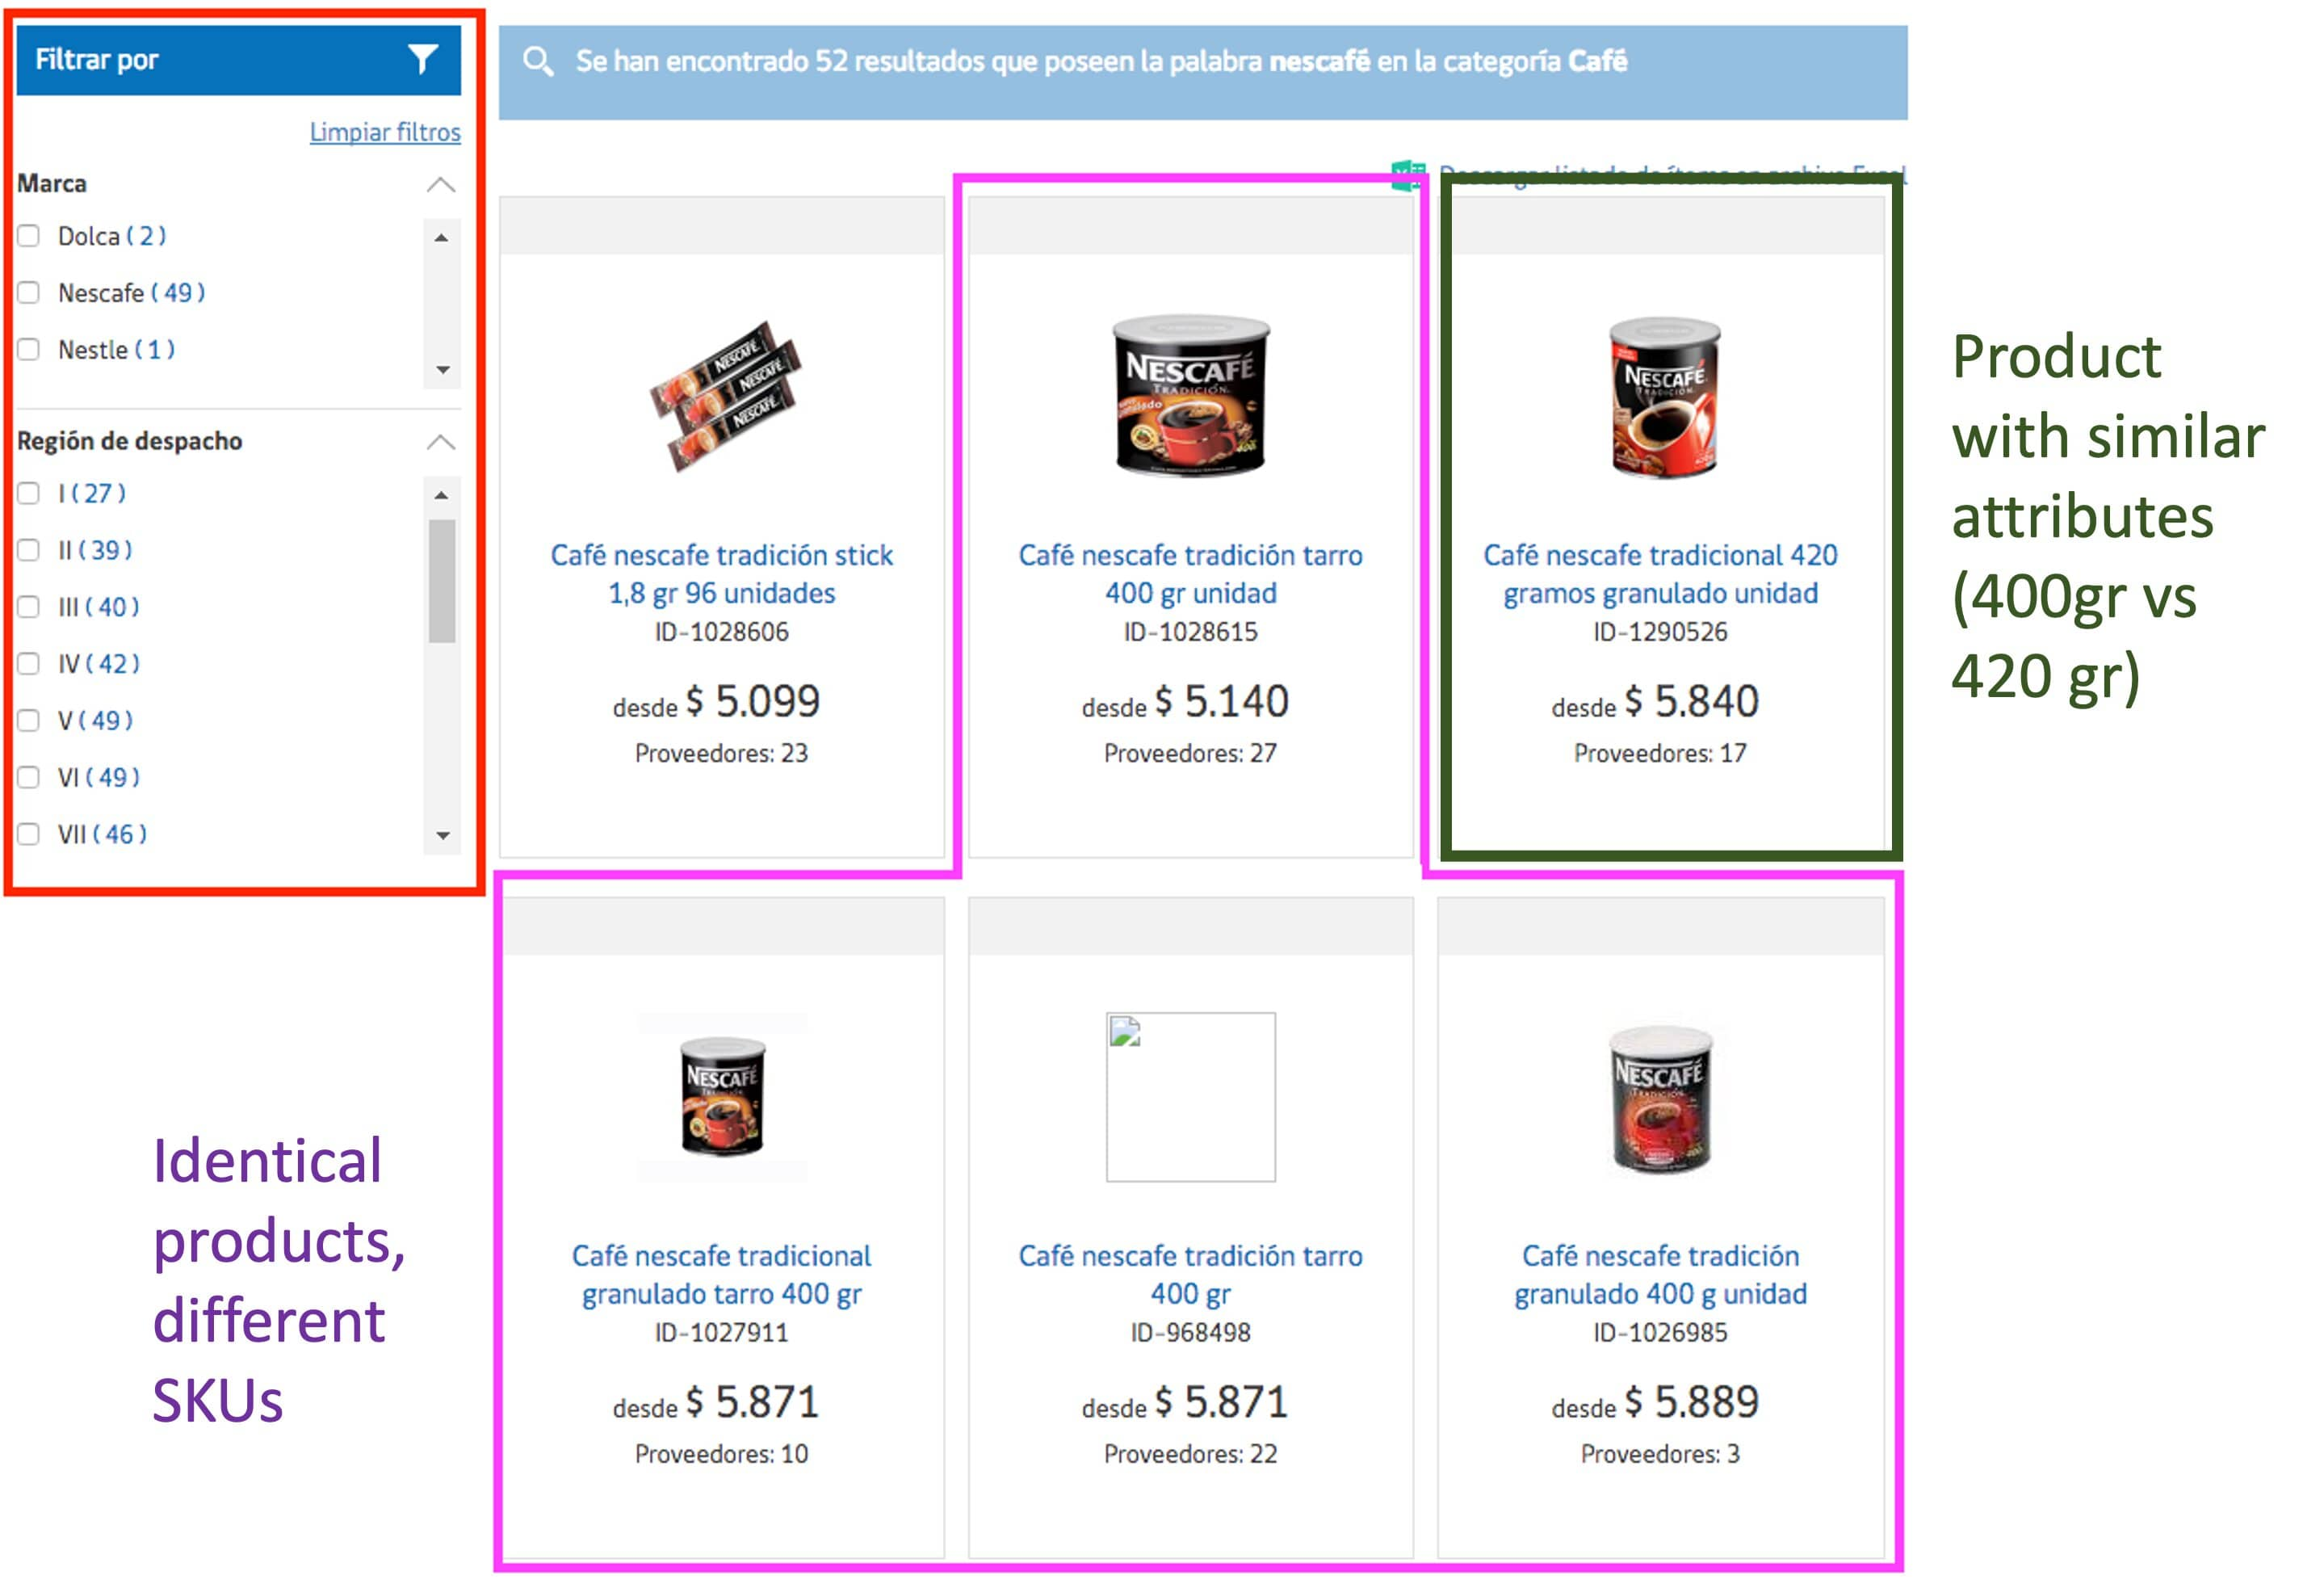
\includegraphics[scale=0.6]{imagenes/procurement/nescafe example.jpg}
    \caption{Example of similar products offered in the operation stage of the FA 2014. The search ``Nescafe'' displays multiple products corresponding to this instant coffee brands. Four products are identical and another one is very similar (with a small variation in the size). None of these products competed among them in the auction stage: they where either considered in separate auctions or added by suppliers as new products during the operation stage. }
    \label{fig:nescafe}
\end{figure}

\noindent{\bf Should FA auctions be more competitive?} Based on the above discussion, it is unclear whether making the rules of the auction more competitive translates to lower government spending. On the one hand, it is true that by making the auctions more competitive, the auctioneer may be able to decrease the awarded bids and hence the ceiling prices. On the other hand, if fewer bids are awarded, then there will be fewer suppliers in the FA, which in turn may decrease the price competition during the operation of the FA. 

{A series of papers employing mechanism design and auction models with incomplete information have been published with the intent of elucidating the aforementioned trade-off. Specifically, \cite{saban2021procurement} and its subsequent paper \cite{Choi22} present stylized models of FAs, primarily focusing on understanding the impact of increasing auction competitiveness by limiting entry into the FA. Their findings indicate that limiting entry into the FA can indeed lead to reduced purchasing prices. This observation is valid even in scenarios where suppliers behave strategically, recognizing that while they might not compete for entry into the FA, they will face competition within the FA to attract demand.}\footnote{{An important simplification in these studies is the assumption that suppliers set a single price, which serves a dual purpose: competing in the FA auction and within the FA itself. This stands in contrast to the more realistic scenario where a ceiling price is set during the auction, with potential discounts applied within the FA. Regardless of this simplification, the models effectively highlight the primary effects of introducing competition into the auction.}}


To shed light on this market design question in a real-world setting, we worked in collaboration with ChileCompra in the design of a new Food FA, where we tested the impact of increasing competition in the auction stage of the FA on public spending. We describe this initiative in the next section.

%\ds{discuss lo que viene.}


%Recall that bid prices to enter the market constitute a ceiling price, allowing suppliers to also compete within the market. Hence, low competition to enter the FA may still lead to low transaction prices if the price competition during the operation of the FA is intense. 



%To shed light on this market design question, we worked in collaboration with ChileCompra in the design of a new food FA, in which we standardize the product catalogue and also tested the impact on public spending of increasing competition to enter the market. We describe this initiative in the next section.

%\input{tables/bids_description/table_competition_fa_2014}


 

% \begin{figure}[H]
% \centering
% \label{fig:operation_fa}
% \includegraphics[scale=.5]{figures/plot_p.bids2014_both.pdf}
% \caption{Number of auctions of Pantry Products by percentage of awarded bids. This distribution excludes auctions in which the total number of bids were awarded.}
% \end{figure}

\section{Designing Framework Agreements to Increase Competition}\label{sec:designFA}


%\input{FAs_to_improve_competition_revision}
% I am including this section here in the text directly

As described above, the 2014 Food FA relied mainly on competition in the operation stage without generating much competition in the auction stage. In order to evaluate the potential for reducing prices through competition in the auction stage, we worked with ChileCompra to test a new design of the 2017 Food FA. Introducing competition to enter the FA required a fundamental change in the auction stage: rather than giving suppliers freedom to define product attributes to bid for, ChileCompra would now precisely define all the characteristics of the products it wanted to purchase. This forces suppliers offering the same products to compete in the same auction and stricter rules would be used to award a reduced number of suppliers. The effective implementation of this strategy required: (1) standardizing products based on measurable product attributes; (2) developing new auction rules that take advantage of this product standardization to induce more competition. Next, we describe these and other improvements that were implemented in further detail. 

\subsection{Implementing the product catalogue} \label{sec:standardization}

The auction stage used to select suppliers in the FA 2014 relied on the suppliers to specify the products in their bids by self-reporting some of the attributes using free unstructured text. As a consequence, products that in practice were very similar in terms of their attributes (or even identical but with different self-reported descriptions) were awarded using different auctions, inducing little competition in this stage (see examples in Table \ref{tab:FA2014_cat_wPrice}). 

To overcome this problem, a key change in the auction stage of the new FA design was to limit the product catalogue to a list defined by ChileCompra, and to disallow suppliers to add their own product specifications. The objective was then to create a structured catalogue of products which included specific verifiable attributes that unambiguously determine each product been auctioned, forcing suppliers to compete in the auction stage. {Following on the examples of Table \ref{tab:FA2014_cat_wPrice}, ChileCompra will only ask for a standard {format and} pack size and all suppliers offering this specific product will compete in the same auction (for some products, separate auctions were created for very large pack sizes to satisfy specific requirements of some government units). For the instant coffee example shown in Figure \ref{fig:nescafe}, the product is defined by attributes related to the brand ("Nescafe Tradición"), format (``400gr'') and pack size (1 unit), forcing suppliers to compete to enter the market for this product, disallowing suppliers that did not win this product to add it during the operation stage. Implementing this strategy required: (1) identifying key attributes that define the characteristics of the products, including differences in quality that would be relevant for buyers; (2) determining which products needed to be included in the catalogue in order to satisfy buyers' needs. Having verifiable attributes for each product is also used to audit suppliers requests to add new products incorporated during the operation stage.}

Given the large number of products (see Table \ref{tab:bid_results_2014b}), it is challenging to construct a detailed product catalogue that would cover the procurement needs of a diverse set of institutions. In order to manage the large complexity of the catalogue, we used Natural Language Processing (NLP) techniques to process the unstructured text of the product descriptions in order to generate standardized attributes for each SKU.  The process is summarized in Figure \ref{fig:catalogue_automation} and described in detail in what follows.

\begin{figure}
 %   \centering
    \caption{\textbf{Standardized catalogue automation using Natural Language Processing.} }
    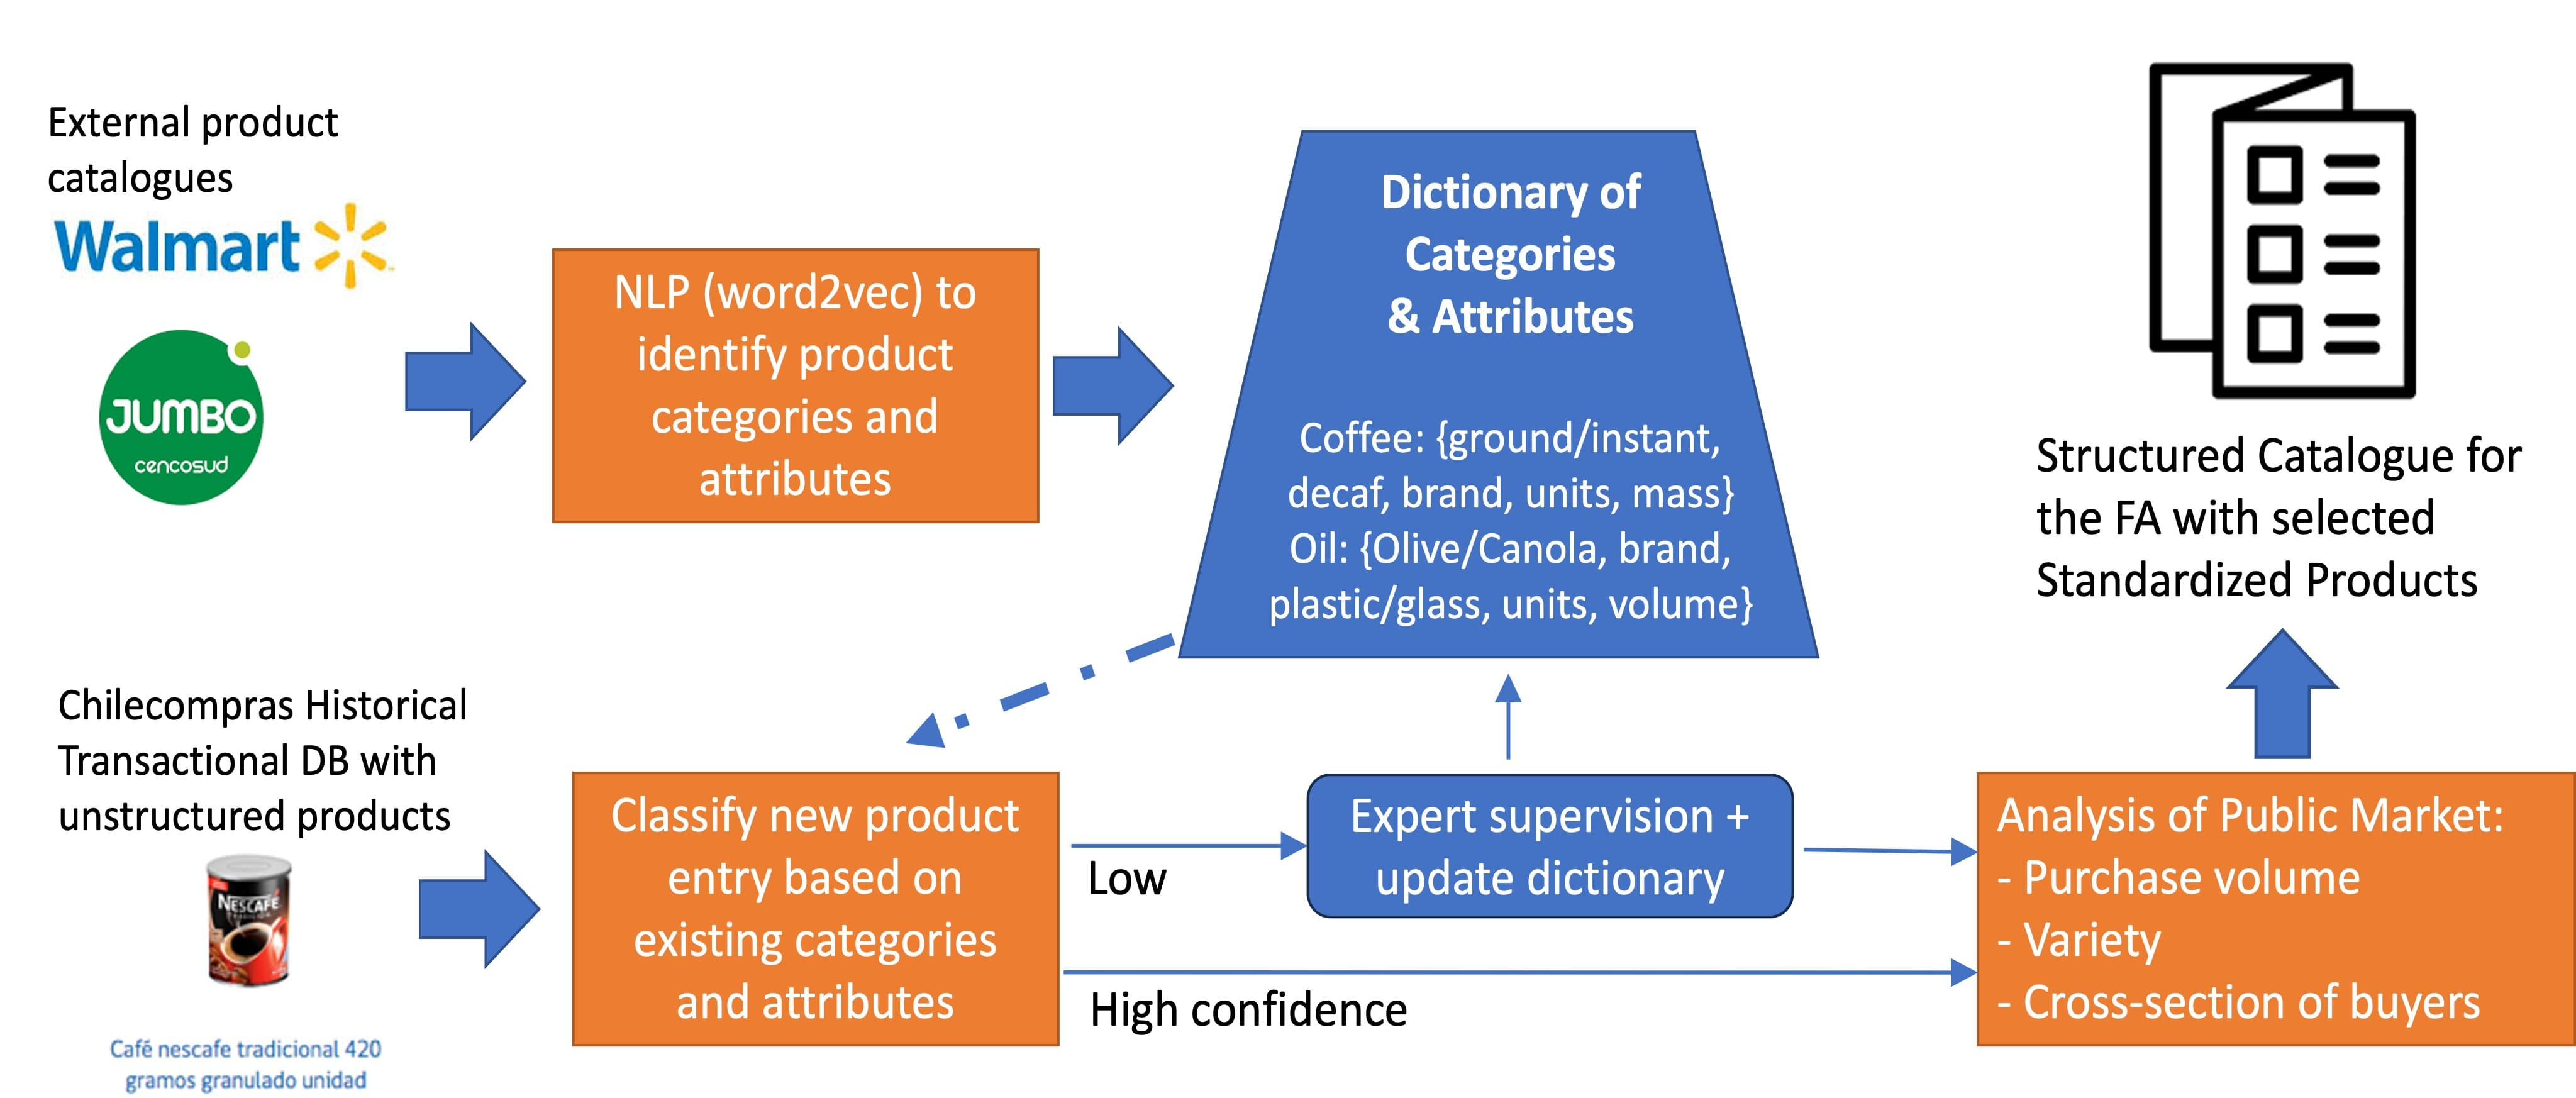
\includegraphics[scale=0.5]{imagenes/procurement/Catalogue_automation.jpg}
    \small{\textit{Notes:} Catalogues from external retailers are used to create a product dictionary, associating each category with specific attributes. A combination of Natural Language Processing algorithms are used to detect attributes for the different product categories. The trained algorithm is then used to identify attributes of products transacted in the FA 2014. This structured catalogue is analyzed to identify products (and their attributes) that are regularly purchased in the public market, which is then used to define the product catalogue for the FA 2017.}
    \label{fig:catalogue_automation}
\end{figure}

First, we collected data from external retail catalogues published online and defined a basic product hierarchy based on this catalogue. We used external catalogues because product descriptions and their categorization were more precise and consistent compared to the product descriptions of products sold in the 2014 Food FA used by ChileCompra. 

Second, we processed the unstructured text of product descriptions in the external catalogues to identify relevant attributes that could be used to standardize products. Figure~\ref{fig:NLP} illustrates this process. The classification involves two steps: (1) identifying the category corresponding to that product (i.e., pasta, coffee, soft-drinks); (2) identifying the specific attribute values that describe products in that category (brand, size, container type, units per package, among others).
The identification of attributes combines unsupervised and supervised methods. In a first pass, we used Word2Vec (\cite{mikolov2013distributed}) to identify words (tokens) that appear within a similar context in the product descriptions. For example, for soft-drinks category the tokens ``300ml",``1.5lts" and ``2000cc" appear in similar contexts in the text. Each token group is revised by a human to assign a corresponding attribute for this product category -- in this example, the tokens describe the \textit{size} attribute of the soft-drink. Because the attribute take numerical values, it is also assigned a \textit{size unit} attribute --  in this example, the values of these attribute include ``lts" (liters) and ``cc" (cubic centimeters). This process results in the definition of a dictionary that contains a set of product categories, each of them with a corresponding set of attributes and their possible values. Using unsupervised methods to process the large number of product descriptions  is essential to scale the construction of this dictionary.

As the catalogue's dictionary gets populated, the NLP algorithm can be used to predict the attributes of a product based on their {text} description, using a measure of distance of each description with those products that have already been correctly classified. These predictions are done sequentially to first detect the product's category and then values associated with each of the attributes for that category. Each prediction is associated with a confidence level, using a pre-specified threshold to decide whether the prediction required a manual (human) inspection for validation or not (see Figure~\ref{fig:NLP}). This approach consisting of hybrid classification using NLP and manual inspection was based on the work of \cite{sun2014chimera} and adapted to the context of our data (see \cite{guerra2019diseno} for details).


\begin{figure}[t]
\caption{Structure of the Natural Language Processing algorithms used to identify attributes from free-text product descriptions, combining unsupervised Machine Learning methods and manual classification}
    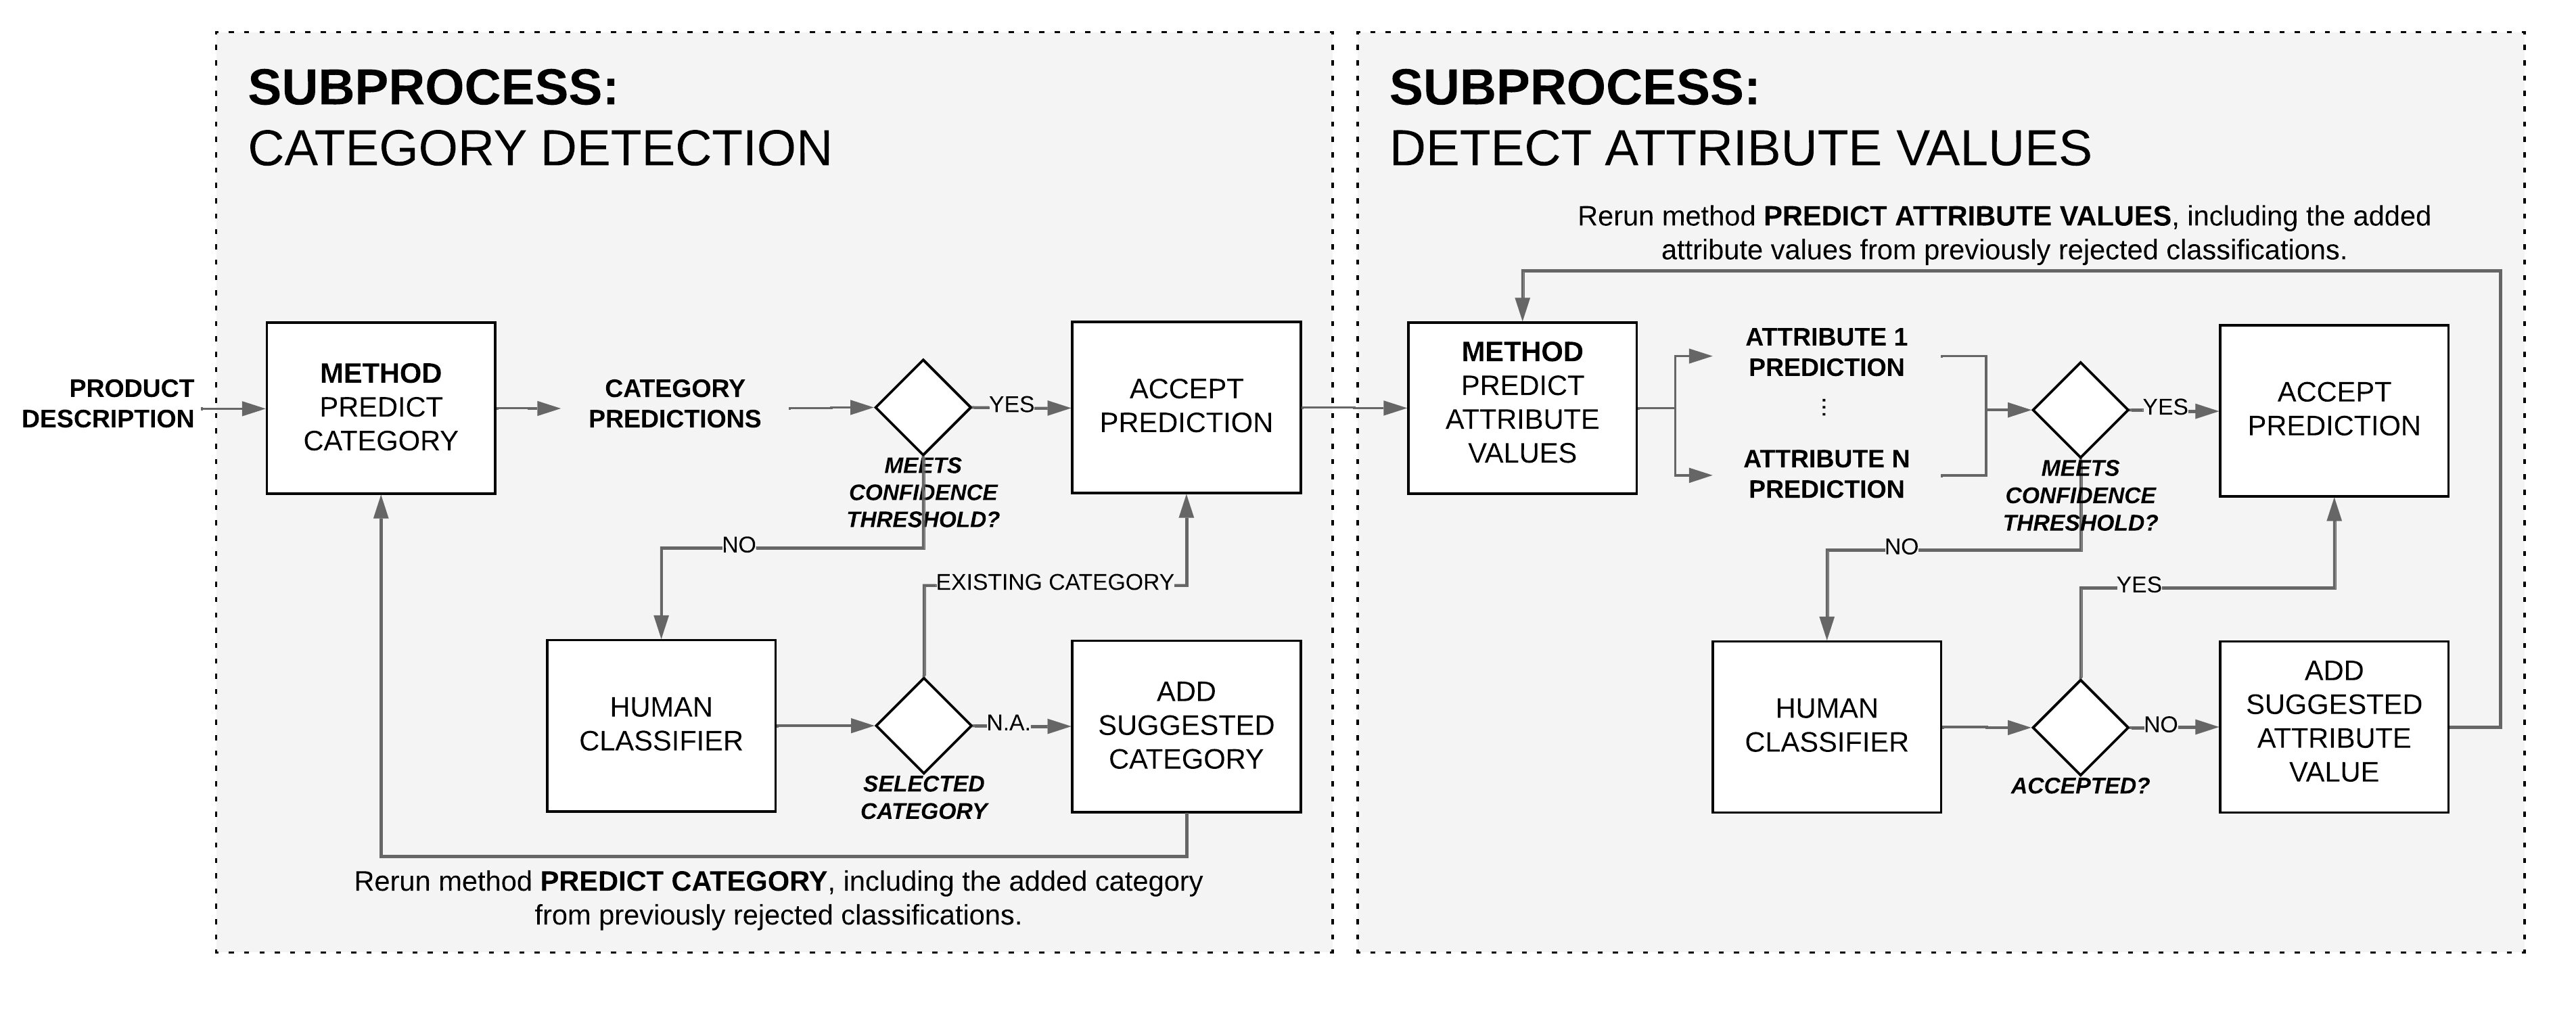
\includegraphics[scale = 0.2]{imagenes/procurement/Attribute detection.jpg}
    \small{\textit{Notes:} Unsupervised algorithms were first used to discover an initial set of product categories and attributes. Unstructured text with product description were processed sequentially using the Category Detection Method to identify the product category and then use the Detect Attribute Values method to identify the value of each attribute assigned to that category. When the predictions do not meet a minimum confidence threshold, the product was revised manually to assign a category and attributes and add the labeled classifications to the predictions. (Source: \cite{guerra2019diseno}, translated by the authors). } 
    \label{fig:NLP}
\end{figure}

As a result of this standardization, each product is uniquely defined by a set of verifiable attributes, which include \textit{category}, \textit{type}, \textit{brand}, \textit{size} and \textit{units/pkg}, plus additional attributes that vary across categories. Table \ref{tab:example_attributes} shows examples of the attributes assigned to product descriptions. \textit{Category} is a generic classification for the product, such as bottled water, canned food, or yogurt.  \textit{Type} refers to a more detailed product specification, a refinement of the  category, which is further specified by a separate \textit{brand} attribute.
The attribute \textit{size} refers to the unit of measurement of a single unit of product, that is, the number of grams (gr.) or milliliters (ml.) in the product container. Finally, products may contain a number of units per package (\textit{units/pkg}). For instance, water might be offered in individual bottles or six packs. Providing this level of detail in the units measurement was important to standardize  bids in the FA auctions.

%\newpiero{Table 2: Example of standardized products for the 2017 Food FA generated using the NLP algorithm. This table shows examples of products in the FA 2017 and their attributes (subcategory, type, brand, format and units.}

\begin{table}[H] 
\caption{\label{tab:ex_prod_2017} Example of standardized products for the 2017 Food FA generated using the NLP algorithm.}
%\centering 
 
 \resizebox{\textwidth}{!}{ 
\begin{tabular}{@{\extracolsep{5pt}} lp{6cm}lp{3cm}p{2cm}ll} 
\\[-1.8ex]
\hline \\[-1.8ex] 
\textbf{Product I.D. }& \textbf{Full Product Description} & \textbf{Subcategory} & \textbf{Type} & \textbf{Brand} & \textbf{Format} & \textbf{Units} \\ 
\hline \\[-1.8ex] 
$1477739$ & sparkling mineral water Next bottle 500 ml.~1 unit & water & sparkling mineral water & Next & 500 ml. & $1$ \\ 
$1445299$ & water-based canned salmon Robinson Crusoe bundle of 3 units 80 gr. & canned-food & water-based canned salmon & Robinson Crusoe & 80 gr. & $3$ \\ 
$1449854$ & ravioli Carozzi meat bag of 400 gr.~1 unit & pasta & ravioli & Carozzi & 400 gr. & $1$ \\ 
$1450212$ & instant coffee Nescafe can 420 gr.~1 unit & tea, coffee & instant coffee & Nescafe & 420 gr. & $1$ \\ 
$1479364$ & probiotic yogurt Uno multifruit bottle 90 ml.~12 units & yogurt & probiotic yogurt & Uno & 90 ml. & $12$ \\ 
$1443780$ &  juice Watt's nectar peach bottle 1,5 lt.~1 unit & juice  &  nectar & Watt's & 1,5 lt. & $1$ \\
\hline \\[-1.8ex] 
\end{tabular}}
 \small{\textit{Notes}: Each product description is decomposed into five attributes: subcategory, type, brand, format, and number of units. Actual product descriptions were originally in Spanish and were translated to English in this example to facilitate the interpretation of the attribute classification.} \label{tab:example_attributes}
\end{table} 

As the algorithm training process was conducted using external catalogues from private retailers, it becomes necessary to specify which of these products should be included in the final catalogue of the FA 2017 auction. This was done by identifying the actual need of these products from the buyers in the public sector, using the trained algorithms to classify the free text descriptions of the products offered in the 2014 Food FA.\footnote{Because some of the description of the products in the FA were offered by small and medium businesses, the algorithm had a lower performance in classifying this products initially. Nevertheless, predictions with low confidence were manually revised following the same procedure described in Figure \ref{fig:NLP}, thereby expanding the dictionary and improving the accuracy of the algorithm on subsequent products.}  In some cases, the algorithm identified new products purchased in the FA 2014 that had not been in the original catalog constructed from external sources.

All the information collected through this product classification was matched with transaction data in the public market to measure the volume of purchases associated with each product and their corresponding attributes. {This provided information about buyers' revealed preferences for the different products.} Moreover, hedonic price regressions (\cite{rosen1974hedonic,greenstone2017continuing}) were used to identify product attributes that were associated to high prices (e.g. specific brands), which could be associated to differences in quality. 

\textit{With all this information at hand, ChileCompra decided which products to include in the final catalogue of the new Food FA, considering adequate coverage to meet buyers' needs, incorporating different levels of product quality .}

{One potential concern of structuring the product catalogue would be a reduction in the variety of products offered in the marketplace. To that end, we analyzed the FA 2014 with the objective of assessing the product variety that was actually included in that catalogue. We focused the comparison on 9000 products of the FA 2014 which correspond to packaged food products -- referred to as \textit{pantry} -- for which it was possible to identify multiple attributes to describe them. For the remaining non-packaged food products -- meat, fresh produced, among others -- it was not possible to identify objective attributes from their description. Hence, we focused the data analysis on pantry products to assess which of these products to include in the new catalogue (for non-pantry, the product selection process was more qualitative and conducted manually by Chilecompra).}

{As expected, many of the auctions ran in the FA 2014 corresponded to products with the same attributes. Of the nearly 9000 packaged products listed in the FA 2014 (each corresponding to a separate auction), it was possible to identify attributes on 7600 of them.  This product categorization reveals that these in fact corresponded to only 2,700 unique products, based on the attributes specified for each product. {Moreover, many of these products had few transactions: the top 2000 products account for 92\% of purchases. Based on this analysis, ChileCompra opted to roughly include comparable 2000 products in the FA 2017 catalogue, which  covered most of the variety of products that were sold in the FA 2014.} 

This structured catalogue based on standardized product attributes was useful to better design the auction stage of the FA and increase competition among suppliers to enter the FA through a bidding process for {specific products}.  We describe the new auction design that leveraged the new structured catalogue in the next section.}


\subsection{Implementing changes to the FA auction rules}\label{sec:auction_rules_changes}

The new auction design incorporated several rules that can be grouped into four major changes (a summary of these changes is also presented in Table~\ref{tab:improvements}).

First, the auction stage is conducted in two phases: technical and economic evaluations. The technical phase verifies specific qualifications of the suppliers based on sales history, infrastructure, and financial statements. After passing the technical evaluation, the second phase focuses in the bid prices to define the awarded bids. This two-phase format is the standard recommended by the World Bank to increase transparency in public procurement (\cite{worldbank})

Second, the structured catalogue generated through the NLP algorithm described in the previous section defined the actual catalogue of products for the 2017 Food FA auction. This selection of products broadly covered the procurement needs of the different government units. The first  stage of the FA is designed as a set of independent auctions, {one per unique product in the catalogue} (defined by the specific verifiable attributes). In contrast to the rules used previously (including the rules of the 2014 Food FA), the new design prevented suppliers from adding new products in the auction stage.

Third, bidding rules were set so that bid prices included the product and delivery costs, with predefined minimum order sizes to reduce transportation costs for the suppliers. As distribution costs can vary significantly across different regions of Chile (urban vs.~rural areas and proximity to centralized warehouses), the country was divided into a set of geographic regions and auctions were run separately for each region for all products. This allowed suppliers to submit different bid prices for the same product across different regions, which were awarded separately.

\textit{All the previous changes were applied for all the product categories in the new FA. }

As a fourth adjustment, we changed the way in which winning bids are decided for each auction. Awarded bidders were set as a percentage of the bids submitted to each auction, with a minimum of 3 awarded bids to ensure an adequate supply. Since this was a major change in the auction rules used historically by ChileCompra, it was implemented through an experimental design  assigning different awarding thresholds for different products categories.  Recall from the discussion in Section~\ref{se:noncomp} that, a priori, it was not clear whether setting a more competitive award rule would result in lower transaction prices.  Providing empirical evidence through an experimental design was critical to measure the impact of increasing competition and inform the design of future FA auction designs. The implementation of this  experiment is described in detail in Section~\ref{sec:impact}.

\begin{table}[]
\caption{Main innovations in the design of the new Food FA.}
    \centering \small{
    \begin{tabular}{p{0.2\linewidth}|p{0.35\linewidth}p{0.35\linewidth}}

 Design attribute & Previous FA  & New FA \\
 \hline
\textbf{Initial product catalogue}
    & Few products, low standardization.  Allows suppliers to define products and add new products during the operation stage.
    & Many products in the initial catalogue. High standardization based on specific attributes, limited options to add new products during the operation stage.
    \\
    \hline

\textbf{Winner allocation}
    & Low competition to enter the FA due to low product standardization. Many auctions with single bids. {Low selectivity in awarding process.}
    & High standardization increases competition to enter the FA. {Experimental design to test different competition levels in the awarding process.}
    \\
    \hline
    
% \textbf{Price uncertainty}
%     & Slow and inaccurate price adjustments during the FA operation. High ceiling prices.
%     & Fast adjustment through time-series forecasting based on objective external market information.

\end{tabular}
} 
    \label{tab:improvements}
\end{table}

In addition to these changes in the auction design, the new Food FA included some additional innovations to facilitate the operation of the FA. A price index mechanism was introduced to reduce suppliers' exposure risk to market fluctuations. Price indexes were adjusted every six months based on external price indexes published by the government statistics bureau (Instituto Nacional de Estad\'isticas).\footnote{See \cite{gur2017framework} for a theoretical motivation of this intervention.} Second, suppliers would face restrictions to add new products during the operation of the FA. Only a limited number of new products were allowed per year, which had to be previously authorized by ChileCompra to ensure that these product were not already offered in the existing assortment.\footnote{To reduce administrative costs of Chilecompra, product descriptions where validated with the NLP algorithms in order to determine if they were already offered in the new FA catalogue.}

The auction rules were published in August 2017, followed by one week of consultations by suppliers. Technical evaluations began in November 2017; technically qualified suppliers began submitting bids starting in March 2018. Winners were awarded in June 2018 and the FA operation started in August 2018.

The auction stage included 52,844 auctions, which received on average 5.3 bids per auction, higher than the 3.4 bids per auction that were received in the 2014 Food FA auction. Recall that the 2017 Food FA auctions were run locally on each region whereas in the 2014 Food FA there were many auctions that covered the whole country; therefore, it was notable that the average number of bids per auction increased in the new FA. {This also explains the increase in the number of auctions.} Moreover, the percentage of single-bid auctions decreased from 51.2\% to 28.7\%, suggesting that the new auction design was effective in inducing more competition in the auction stage. The next section describes the methodology used to measure the impact of this new auction design on prices and procurement expenses.


% \begin{figure}[H]
% \centering
% \includegraphics[scale=1]{figures/operation_fa_img.pdf} 
% \caption{\label{fig:FA_timeline}}
% \end{figure}

\section{Measuring the impact of increasing competition in the FA auction} \label{sec:impact}

A fundamental change in the new Food FA was the construction of a structured catalogue defined by Chilecompra, which is used to define separate auctions for each product to award the suppliers that enter the FA marketplace. There was consensus among the stakeholders at Chilecompra that this new catalogue would increase efficiency in several dimensions: lowering the administrative costs of processing the bids, reducing redundancy of products and improving the organization of the catalogue in the marketplace. Hence, the standardization of the catalogue was implemented across all the product categories of the new 2017 FA.

However, there was debate on how much to intensify competition in the auction stage, {given the trade-off between reducing ceiling prices at entry and promotions in the operation stage.}\footnote{It is also common for the non-awarded suppliers to complain and file grievances on the awarding process; a more competitive entry would increase the risk in this dimension if price reductions were not significant.} 
 It therefore became critical to provide convincing evidence of the actual impact of increasing competition in the auction stage, for which \textit{we implemented the new Food FA  through a field experiment focused on measuring the effect of different levels of competition}. This approach consisted in defining two alternative awarding rules -- with high and low competition in the auction stage -- which were randomly assigned to product categories. We then compared the bids and prices of these products in the FA 2017 relative to the FA 2014,  which required matching products with similar attributes across the two FAs. This sample of matched products was used to conduct a difference-in-differences regression to measure the impact of inducing more competition in the auction stage. Note that all the products in the new FA were part of a structured catalogue, therefore the experiment focuses in measuring the \textit{incremental effect} of increasing competition in an FA were all products are defined through a standardized set of attributes. This section describes the design and implementation of this field experiment, and the econometric models used to measure its impact on bids and prices.

\subsection{Experimental design}

The implementation of the new Food FA was designed to measure the implications of increasing  competition in the auctions used to select the suppliers that enter the FA. This was conducted through an experimental design where each product auctioned in the new Food FA was assigned to one of two possible groups based on its awarding thresholds. In the \textbf{Noncompetitive (baseline) group} the lowest 80\% of all received bids in the auction were awarded and included in the FA assortment. In the \textbf{Competitive (treatment) group}, only the lowest $20\%$ of all received bids in the auction were awarded and included in the FA assortment.

In both cases, the rules imposed a minimum of three bids awarded so as to reduce potential risks in the supply (due to limited availability, delays in the distribution, among etc.). For example, if an auction in the competitive treatment received 10 bids, then the three lowest-bid products would be added to the FA, effectively awarding  30\% of the bids (not 20\%). All the other changes in the rules of the auction described in Section~\ref{sec:auction_rules_changes} were applied to \textit{all} auctions regardless of whether they were assigned to the baseline or the competitive treatment. Hence, the randomized assignment of this treatment allowed us to isolate the impact of this design variable on the outcomes of interest: inducing more competition to enter the market. 

Product categories were assigned randomly to the competitive and noncompetitive treatments. We chose to make the assignment at the product category level so as to avoid having two close-substitute products being assigned to different competitive treatments alleviating interference effects and concerns regarding {the Stable Unit Treatment Value assumption (SUTVA) required to identify a global treatment effect.} Of the 45 proposed assignments, ChileCompra changed one assignment from competitive to noncompetitive and one from noncompetitive to competitive.\footnote{Rice was moved from the competitive to the noncompetitive treatment in order to increase the likelihood of allocating to local suppliers. Coffee and Tea was moved from the noncompetitive to 
 the competitive treatment because it was considered an important category to enhance competition, given the large volume of purchases.}

 \subsection{Matching products across FAs}\label{subsec:matching}

 We sought to compare the bids and prices of products in the old and new FA, as well as of the two competitive treatments to measure the impact of the new design. {To do so, we relied on the product characterization provided through the NLP algorithms described in Section \ref{sec:standardization}. Recall that products in the old and new FA were standardized by identifying comparable product attributes from the information contained in the product description. Because some of the products changed their format across years, we generated groups of products that were ``close'' in the space of attribute values. For example, bottles of 950 ml. and 1 liter were considered to be similar in that attribute. In general, two products were associated with the same standardized product if: (i) they shared the same category, product type, brand, and format (e.g., grams); and (ii) the percentage difference between the format values was less than 20\%. }
 
 {While in principle we could apply this methodology to any product in the catalogues, in some product categories of the FA 2014 product description did not contain sufficient information to identify attributes and NLP was unable to categorize them correctly. Consequently, we focused the econometric analysis on pantry products (corresponding to packaged product categories) and excluded fresh bread, vegetables, fruits, seafood, meat products, and others perishable product categories for which the attributes detected in the FA 2014 were not sufficient to describe the product's quality.\footnote{ To be clear, these categories where included in the 2017 FA, where all the relevant product attributes describing quality and other characteristics were specified in detailed. The reason for excluding them from the econometric analysis was due to the challenge in matching these products with poor product description in the old FA.} For most pantry products, product descriptions in the FA 2014 were sufficiently detailed to identify attributes through the NLP algorithms; this selection includes 35 product categories, which comprised our initial sample for analysis.}
 
 Table \ref{tab:matching_results} shows the results of this attribute identification and matching across the two FAs. For the FA 2014, products with identified attributes---7,642 out of 8,937 products---accounted for more than 90\% of the sales of {pantry products in the FA}, which shows the high degree of effectiveness of the product standardization algorithms  {for these product categories}. Using these attributes to identify similar products, we found that these 7,642 products actually corresponded to 2,703 \textit{unique} products. Of these 2,703 unique products, 928 products had a match with a product in the 2017 Food FA (based on the criteria described above). These matched products account for about 68\% of the sales of pantry in FA 2014, and 74.1\% in the FA 2017.  These matched products defined a representative sample that was used to evaluate the impact of the changes in the FA design, by comparing the prices of the same standardized products across the old and new FAs.
 
 
 \begin{table}[H]
\centering 
\renewcommand{\TPTminimum}{\linewidth}
\small{
\begin{threeparttable}
\makebox[\linewidth]{%
%\setlength\extrarowheight{-3pt}
\begin{tabular}{@{\extracolsep{-5pt}} p{8cm}ll} 
\\\hline 
 & \multicolumn{2}{c}{No. of Products (\% sales)}\\ 
 \cline{2-3}
 & FA 2014 & FA 2017 \\ 
\hline \\[-2.5ex] 
Total number of \textit{pantry} products & 8,937 (100\%) & 3,789 (100\%) \\
Products with identified attributes & 7,642 (92.4\%) & 3,704 (97.3\%) \\
Unique products based on selected attributes & 2,703 (92.4\%) & 2,027 (97.3\%) \\
Matched products across FAs & 928 (68.2\%) & 928 (74.1\%) \\ 
\hline 
\end{tabular}}
% \begin{tablenotes}
%   \small
%      \item \textit{Note:} This table summarizes the results of the product standardization process. We say that a SKU is feasible if all the following attributes were identified: \textit{subcategory}, \textit{type}, \textit{brand} and \textit{format}. The mentioned attributes define a unique Standardized product.
%    \end{tablenotes}
\end{threeparttable}
}
\caption{Product identification summary for all \textit{pantry} products {-- packaged products which can be described through standardized attributes --} in the 2014 (old) and 2017 (new) FAs. The last row counts unique products that were found in both FAs.}
\label{tab:matching_results}
\end{table} 

 
 \subsection{Hypotheses}
 
 The main goal of inducing more competition in the auction stage is to generate lower transaction prices and thereby reduce procurement costs. There are alternative mechanisms that can lead to this price reduction. First, awarding bids to a smaller fraction of bidders---the competitive treatment condition in our experimental design---should lower the cutoff bid price, thereby leading to lower \textit{awarded bids}. Moreover, this increased competition in the auction stage might also lead suppliers to bid more aggressively, leading to lower \textit{submitted bids}, which should further reduce the awarded bid prices. Overall, we expect that auctions in the competitive treatment should have lower awarded bids relative to the noncompetitive treatment.
 
Moreover, recall that the auction stage of the FA sets the ceiling prices that suppliers can charge, but that suppliers can further lower the prices during the operation stage through price promotions. As previously discussed, while awarding a smaller number of bids may decreases ceiling prices, it is not clear that it also decreases the prices that are offered during the operation stage of the FA. Hence, 
fewer participants in the FA could potentially increase the \textit{posted} prices that suppliers set in the online platform. This increase in posted prices may also lead to higher \textit{transaction} prices at which buyers purchase these products.

Based on this discussion, we postulate the following hypotheses that we test in the next section:
 
\noindent \textit{\bf Hypothesis 1.} \textit{Lower ceiling prices}: Awarding a smaller number of bidders leads to lower awarded bids.

\noindent \textit{\bf Hypothesis 2.} \textit{Prices for the competitive treatment are lower}: {Awarding a smaller number of bidders, leads to lower posted and transaction prices.} 

 \noindent \textit{\bf Hypothesis 2 alt.} \textit{Prices for the competitive treatment are \textit{not} lower}: {Posted and transaction prices are not lower in the competitive treatment. Price competition in the FA operation may compensate for less competition in the auction.}

 
\subsection{Econometric model}

We conducted a difference-in-differences regression to measure the effect of increasing competition in the auction stage, distinguishing the alternative mechanisms discussed in the hypotheses formulation. Specifically, we sought to estimate the causal effect of the competitive treatment condition on submitted and awarded bid prices in the auction stage and posted and transaction prices during the operation stage.

\paragraph{Auction stage: Analysis of bids.}
First, we focus on studying the effect of the new FA design and the competitive treatment on the auction bids. As we explained above, bid prices correspond to the ceiling prices that the suppliers can charge during the operation of the FA. 

Let the index $t\in\{\text{Old},\text{New}\}$ represent the old (2014) and the new (2017) Food FAs, respectively.  Let $b_{ijrt}$ represent the bid offered in FA $t$ by supplier $j$ to provide product $i$ in region $r$, including shipping.\footnote{Recall that some auctions were run at the national level in  the FA 2014. However, suppliers must specify a shipping rate for all regions they seek to supply, which is used to calculate the bid price for each region.} Define $B^{med}_{irt}$ as the \textit{median} bid across all supplier bids submitted in the FA for that product-region-FA combination. In calculating this median bid price, we considered alternative methods for discarding extreme prices that could be generated by bidding mistakes or unrealistically aggressive bidding. For the main results we used a modified Tukey rule \citep{Tukey1977}, described in Appendix \ref{app:data}. To make the bids for the 2014 and 2017 Food FAs comparable, all prices for 2014 were adjusted using the CPI food price index. In addition, we normalized bid prices so that they represented bid prices per unit. See  Appendix \ref{app:data} for further details on data pre-processing. 

The following difference-in-differences specification is used to estimate the effect of the competitive treatment condition ---denoted by the indicator variable $Comp_{i}$--- on bid prices:
\begin{equation}
    \log (B^{med}_{irt}) = \delta_r + \gamma_i + \alpha New_{t} + \beta New_{t}\times Comp_{i} + \varepsilon_{irt} \ ,
    \label{eq:reg_sub_bid}
\end{equation}

\noindent where $New_t$ is an indicator equal to one for the new FA and $\delta_r$ is a region fixed effect. The sample is comprised of all products $i$ that were matched across the old and new FAs based on similar attributes, and the regression includes a product fixed effect $\gamma_i$. {The error term $\varepsilon_{irt}$ represents other idiosyncratic unobservable factors that affect bid prices of each product across FAs and  regions.} The coefficient $\alpha$ measures the average differences in bid prices between the old and new FAs for the noncompetitive baseline group. The key parameter of interest is $\beta$, the coefficient capturing the incremental change in bid prices for the auctions in the competitive treatment condition in the new FA.

Recall that $B^{med}_{irt}$, which is the median across all \textit{submitted} bids, measures whether the competitive treatment affects the bidding behavior of the suppliers.  Any changes in the submitted bids should carry over into the winning bids. Furthermore, the competitive treatment condition also lowers the cutoff point of the winning bids, which can lead to lower awarded bids even when submitted bids remain constant. Hence, we also estimated regression \eqref{eq:reg_sub_bid} using the median among \textit{awarded bids} as the dependent variable. Taken together, these models allow us to test Hypothesis 1, by measuring the effect of less competition in the auction stage on the winning bids and identifying what part of this reduction is due to changes in bidding behavior.



\paragraph{Operation stage: Analysis of prices.}
While the bids constitute a ceiling on the price that suppliers can charge during the operation of the FA, the ultimate goal is to reduce posted and transaction prices, which translate directly into procurement savings. To conduct this analysis, we assembled a weekly panel dataset including prices posted in the online platform and the actual transacted prices from purchasing orders. Let $p_{ijrtw}$ denote the average posted prices by supplier $j$ for product $i$ in region $r$ during calendar week $w$ in FA $t$. As with the bids, we calculated the {\em median posted price} for a product across all suppliers during that week, denoted by $P^{med}_{irtw}$. That is, $P^{med}_{irtw}$ denotes the median price at which product $i$ could be purchased in region $r$ during calendar week $w$ under the operation of FA $t$ in the period listed above. 

We estimated the panel regression:
\begin{equation}
    \log (P^{med}_{irtw})= \delta_r + \gamma_i + \tau_{wc(i)} + \alpha New_{t} + \beta New_{t}\times Comp_{i} + \varepsilon_{irtw} \ ,
    \label{eq:reg_op_posted}
\end{equation}
\noindent where $\delta_r$ and $\gamma_i$ are region and product fixed effects respectively, $\tau_{wc(i)}$ is a product category-specific calendar week dummy variable to capture potential seasonality ($c(i)$ indicates the category of product $i$). {The error term $\varepsilon_{irtw}$ represents other unobservable factors that affect prices during the operation stage.}


To analyze actual expenditures, we estimated model \eqref{eq:reg_op_posted} using as dependent variable the \emph{median transaction price} across all units that were bought during a given week. To calculate the median, we considered each unit bought as one observation. For example, an order with $n$ units for the same product is considered as $n$ different observations in the median calculation. In this way, the median considers the quantity of products sold at each price level. Notice that this panel is unbalanced because some products were not sold  every week.

Both panel regressions were estimated with data from 13 months prior to the operation of the new FA (August 2017 to August 2018) and the first 13 months of operation (September 2018 to September 2019).\footnote{Using a window of 13 months ensured that all 52 calendar weeks are considered.} Prices are adjusted for inflation according to the monthly CPI index for Food and Non-alcoholic Beverages. In addition, we eliminated outliers by applying the same procedure used for bid prices.

\subsection{Estimation results}

Table \ref{tab:main_results} shows the main estimation results showing the impact of the change in the level of competition  in the  auction stage on bids and prices. Columns (1) and (2) show the effect on submitted and awarded bids (regression \ref{eq:reg_sub_bid}); columns (3) and (4) show the effect on posted and transaction prices (regression \ref{eq:reg_op_posted}). Appendix \ref{app:robustness} contains robustness analyses and alternative regression specifications. The results obtained from these alternative regression specifications are qualitatively similar to the ones obtained with the main  specifications here.


\begin{table}[H] \centering 
\footnotesize 
\setlength\extrarowheight{-1pt}
\begin{tabular}{@{\extracolsep{-10pt}}lccp{1cm}cc} 
\toprule
 & \multicolumn{2}{c}{\textit{Bids}} & & \multicolumn{2}{c}{\textit{Prices}}\\ 
\cline{2-3} \cline{5-6} 
 & Submitted & Awarded && Posted & Transaction \\ 
& (1) & (2) && (3) & (4)\\ 
\hline
\\
 New FA & $-$0.141$^{***}$ & $-$0.055$^{***}$ & & $-$0.025$^{***}$ & 0.004$^{***}$ \\ 
  & (0.006) & (0.007) & &(0.001) & (0.002) \\
  \\
 New FA $\times$ Competitive & 0.002 & $-$0.081$^{***}$ & & $-$0.092$^{***}$ & $-$0.082$^{***}$ \\ 
 & (0.010) & (0.013) & & (0.001) & (0.002) \\ 
 \\
\hline 
Observations & 12,349 & 11,382 & & 973,195 & 180,421 \\ 
R$^{2}$ & 0.923 & 0.892 & & 0.961 & 0.974 \\ 
Adjusted R$^{2}$ & 0.920 & 0.887 & & 0.961 & 0.974 \\ 
\bottomrule
\multicolumn{5}{l}{\textit{Note:}  $^{*}$p$<$0.1; $^{**}$p$<$0.05; $^{***}$p$<$0.01} \\ 
\end{tabular} 
\caption{\label{tab:main_results} Main estimation results measuring the effect of the new FA design and the level of competition in the auction stage on bids and prices. All the specifications include product and region fixed effects. {For regressions with Bid prices, some auctions were not awarded and therefore the number of observations drops when using awarded bids (column (2)). Regressions with posted and transaction prices (columns (3) and (4)) include product category-specific calendar week dummies to control for seasonality. Since not all products are sold every week, the transaction price regressions have fewer observations relative to posted prices.} Robust standard errors for each estimated coefficient are reported in parentheses for all the models.}
\end{table} 


 The estimation results in columns (1) and (2) suggest that the baseline groups in FA 2017---which were awarded 80\% of the bids---exhibited lower bids relative to the FA 2014: the \textit{New} coefficient estimates that submitted bids were reduced by 14.1\% and awarded bids were reduced by 5.5\%. Although part of this effect may be attributed to changes in the auction design,  it is not possible to disentangle this effect from other external factors, such as changes in food prices or other fluctuations in the open market. Hence, we cannot interpret $\alpha$ as a causal effect of the new design on prices.%\todoMO{Added a line to explain the reasoning}
 
 The effect of the competitive treatment ---which was induced through a randomized experimental design--- can be interpreted as a causal effect of inducing more competition in the auction stage of the FA. The interaction term $New\times Comp$ shows that auctions that had lower thresholds for assigning winners led to lower awarded bids ---on average 8.1\% lower (column (2))--- providing support for Hypothesis 1. However, there appears to be no effect on the bids submitted by the bidders: in column (1) the coefficient of $New\times Comp$  is small and not statistically significant. This suggests that the reduction in the price of the awarded bids was not induced by changes in bidding behavior across the different auction rules (i.e., competitive or noncompetitive) but rather due to the lower awarding threshold applied in the competitive treatment group. {Note that the regressions with submitted bids include some auctions that were not awarded, hence the sample size is larger relative to the analysis with awarded bids. Appendix \ref{app:robustness} shows the estimation using the sample of awarded auctions, which yields similar results.}

In terms of prices, the results suggest that posted prices were lower across all products in the new FA design relative to FA 2014, showing a 2.5\% reduction in the price of the products in the noncompetitive treatment and an additional 9.2\% reduction of those in the competitive treatment {(see column (3) in the table)}. Overall, the reduction in posted prices of products in the noncompetitive treatment is substantially smaller than the reduction in the ceiling prices (determined by the awarded bids); that is, the pass-through from ceiling to posted price is not one-to-one. 
For the noncompetitive products, posted prices decreased by 2.5\% relative to the FA 2014, about half the 5.5\% decrease observed for the awarded bids. 

Products in the competitive treatment had posted prices that were 11.7\% lower (0.025 + 0.092) relative to the FA 2014, compared to a 13.6\% (0.055 + 0.081) drop in the awarded bid prices. One potential explanation is that in the old FA, even though ceiling prices were higher, this lack of competition in the auction stage was partially compensated for by more competition in the operation stage of the FA, as showcased by the fact that suppliers were frequently running price promotions. Overall, the new FA design combined with a more competitive auction stage was effective in reducing posted prices, and the effect is statistically and economically significant.

More importantly, the estimates on transaction prices (column (4) in Table \ref{tab:main_results}) reveal that the reduction in posted prices for the competitive treatment also translates into a significant reduction in transaction prices, in the order of 8\%, relative to the FA 2014. However, the {change} on transaction prices for the noncompetitive group is negligible. Taken together, these results provide support for Hypothesis 2: inducing more competition in the auction stage was effective in reducing posted and transaction prices, thereby lowering procurement spending for the government.  The savings in the government procurement cost amounted to US\$3.6 million  yearly if we  consider only the treatment group and to US\$11 million yearly if we extrapolate to the
entire Food FA.\footnote{The extrapolation more than doubles the savings because, as we explained before, there were many non-pantry product categories not considered in the experiment.} The results highlight the importance of introducing  a competitive entry stage to achieve reductions in procurement costs when using FA purchasing mechanisms.



\section{{Generalizing the New FA Design, Impact and Transferability}}

% \subsection{Transferability to other Framework Agreements}

 
 Through the pilot study just described, we identified important steps that were fundamental to induce competition upon entry and for the efficient operation of the FA:  product standardization and defining the catalogue of products to be procured. These steps have been adopted as part of the standard operating procedure used by ChileCompra in the design and implementation of FAs, which were formally included in the new regulation on public procurement (\cite{leycompras}). In addition, the experimental design used in the Food FA provided evidence in support of inducing more competition in the auction stage of the FAs. Based on this, ChileCompra adopted a new strategy for the design of all the FAs that were implemented after the Food FA.
 With this motivation, we collaborated with ChileCompra during August 2019--February 2020 with the objective of transferring the tools and know-how developed in the Food FA to the design of several new FAs: for office supplies, computers, office furniture, household cleaning, and hardware. This transferability was supported by a government grant, aimed at facilitating the adoption of the best practices that were identified in the Food FA pilot study.\footnote{Fondef Project ID16I10122, ``Diseño De Una Plataforma Para La Implementación De Convenios Marco Competitivos," directed by Marcelo Olivares.}

\noindent{\bf Competitive auction rules.} 
Similarly to our Food FA re-design, the new FAs had a two-stage design: a first, selection stage based on technical criteria followed by a second, competitive stage conducted through an auction based on prices. 
The design of the auction stage included a structured product catalogue, developed by ChileCompra, specifying detailed product attributes that uniquely identified the products to be auctioned. Some of these catalogues were constructed based on catalogues from the open market and processed using NLP tools (which included some extensions of those used for the Food FA). 

Moreover, the awarding rules were uniformly changed to induce more competition relative to previous FAs. 
In some of the new FAs, awarding rules were based on a fixed number of winners per auction. For example, for the Computers FA (2020), products were grouped into quality categories where the $X$ lowest bids in each quality category were awarded (the number of awardees $X$ varied between 10 and 20 across the Desktop and Laptop Computer categories, based on the potential number of suppliers). Office Furniture and Office Supplies FAs used a similar awarding criteria. For other FAs, awarding rules were defined as a percentage of the submitted bids. For example, for the Household Cleaning FA, the lowest 30\% of the received bids were awarded and  for Industrial Cleaning Products FA, where products  are bought in larger volumes, the cutoff was set at 10\%. The Hardware Products FA used similar awarding criteria.


\noindent{\bf Product standardization and product catalogue.} As discussed in Section~\ref{sec:auction_rules_changes}, to implement a competitive yet meaningful auction, it is useful to have a standardization of the products to eliminate the differentiation introduced by suppliers that would reduce the competition. The NLP methodology developed in the pilot study was further developed to improve its accuracy and packaged into a stand-alone application programming interface, funded by government grants aimed at technological transfers to the public sector. This interface was transferred to ChileCompra and made available as open source code that could be used in other public sector and non-profit applications.\footnote{The source code is available at the repository \texttt{https://github.com/rguerral/catalogador\_standalone}. }

After the implementation of the Food FA, ChileCompra changed its procurement strategy and opted to focus FAs on categories for which it was possible to describe products through observable attributes. Categories for which it was not possible to describe products through a structured catalogue (e.g., catering services, training programs) were moved from FAs to other procurement mechanisms such as auctions or direct purchases. {This led to fewer products and services being available through FAs, but these FAs exploited product standardization to generate a more competitive awarding process and thereby achieve lower prices. As a consequence of this new strategy, the share of purchases conducted through FAs was reduced from 23\% in 2018 to 11.6\% in 2021 (because there were fewer categories), but product categories operating with the new FA design were actively used by buyers.}

{\noindent{\bf Impact.}} The entire process of defining a structured product catalogue (using algorithmic NLP methods), made the design and evaluation process more efficient, thereby reducing administrative costs. The methodology for constructing standardized catalogues and introducing higher levels of competition in the FA auction stage was implemented in subsequent FAs, which in 2022 amounted to US\$800 million worth of purchases (including the Food FA).  If we were to extrapolate the treatment effect on transaction prices to these FAs, the total savings would amount to $8\% \times 800 = \textup{US}\$64$  million per year.%\todoMO{Changed the calculation}
%\subsection{Impact beyond the design of FAs}

In addition, the adoption of catalogue standardization in the design of FAs aimed at generating competition in the auction stage also enabled innovations during the evaluation and operation stage of the FA. 
First, reducing the amount of unstructured text product description enabled a more automated process for submitting and evaluating the bids. A web server was developed to receive bids from suppliers in a standard format, providing information on product attributes, prices, and other bid variables that could be used in more complex auction formats. These improvements significantly reduced the work required by suppliers to submit bids and minimize errors in the submission. This bid validation process was implemented as a stand-alone application available in open source to the public.\footnote{The source code for the bid validation interface is available in the following repository \texttt{ https://github.com/rguerral/site\_validador}. }

Furthermore, product standardization led to more structured transaction data, leading to more amenable data analysis conducted during the operation of the FA. In particular, product attributes could be used to identify groups of substitute products and compare their prices, {a key feature to develop an effective search ranking algorithm}. This was also used to develop a monitoring system to measure \textit{overspending} by government units, estimating potential savings that could be achieved by switching to substitute products with lower prices. Savings due to this monitoring system were estimated in the order of 1.5\% of expenditures, equivalent to  US\$12 million if we use the overall 2022 FA expenditures as a baseline (\cite{dipresFEI}).


\noindent{\bf Beyond ChileCompra.}
Public procurement is an important activity: among OECD countries, public procurement ranges between 20\% to 40\% of all government expenditures and between 5\% to 18\% of the countries' GDP (\cite{OECD2017_PP}). FAs are widely used across governments' central procurement agencies, and therefore, increasing efficiency of these purchasing mechanisms can have a sizeable impact on public spending. The findings of our work can be extended to any country having a central procurement agency to coordinate public purchases. Note that all OECD countries report to have a central procurement agency (\cite{OECD2015_CPB}).

In fact, some of the co-authors of this work have been advising other governments in Latin America to implement similar strategies for FAs. On a recent project (April-June 2023), we collaborated with the Ministry of Finance of Peru to evaluate the implementation of FAs, creating structured catalogues to facilitate price comparisons and generate more competition in FAs and other procurement mechanisms. We are currently in conversations with the central procurement agency of Paraguay to initiate a project that replicates the work conducted in collaboration with ChileCompra, helping them to develop a structured catalogue for FAs and designing mechanism that exploit this standardization to increase competition. In addition, through our extended collaboration with ChileCompra, we have been presenting the findings of this work to other countries and institutions (eg. OECD committees and Mexico's procurement body). We hope that these endeavors will have a real practical well impact beyond ChileCompra.

Finally, the findings also carry implications for the recent efforts in U.S. federal procurement to centralize purchasing and reduce costs, such as those outlined in the Federal Information Technology Acquisition Reform Act (FITARA).\footnote{https://www.cio.gov/policies-and-priorities/FITARA/} As procurement processes become more centralized, there is an optimal scale at which investment in technology, such as the one required to build well-structured catalogs,  becomes feasible. In such scenarios, possessing well-designed FAs, like the ones described in this work, could be a strategic choice. Different buyers within an agency can exploit the variety that a well-structured FA provides, while the centralization provided by the FA can leverage purchasing power and reduce the agency's spend.

\noindent{\bf Conclusions.} Our work shows the value of enhancing competition in FA auctions. Moreover, we provided important guidelines on how to implement FAs in practice, which have since been adopted by ChileCompra in the design of other large FAs used to purchase products and services worth US\$800 million per year. We generated decision-support tools that are now actively used by ChileCompra to improve their procurement processes beyond FAs and being considered by governments from other countries. Overall, we believe this project showcases how  market design together with machine learning can greatly improve market outcomes. 



\chapter{The Social Divide of Social Distancing: Shelter-in-Place Behavior in Santiago during the Covid-19 Pandemic}

\section{Introduction}
In the face of the global Covid-19 crisis, governments around the world have rushed to design and implement mitigation strategies to contain the pandemic. Most countries have continuously asked the population to practice physical distance -- in particular, to shelter in place -- and have adopted more radical measures of mandatory lockdowns
to  flatten the curve of infections and prevent a collapse of the healthcare system \citep{hsiang2020effect}. However, the effectiveness of the adopted measures in terms of mitigating the spread of the virus may vary significantly across the population groups where they are implemented \citep{allcott2020polarization,lamb2021differential}. Our work seeks to identify factors that help to explain the heterogeneous effects of social distancing  in the capital of  a developing country:  the city of Santiago, Chile, with a population of around 7 million. With this evidence we shed light on general policy prescriptions to contain the pandemic in large urban cities that exhibit significant socioeconomic  disparities \citep{florida2017new}.

Chile's first case, a traveler from Singapore, was detected on March 3, 2020.  The date coincides with the start of the working and academic year (January and February correspond to school summer vacations). The virus spread rapidly, with an average doubling time of 2--3 days in the first few weeks. On March 15, the government mandated the closure of all schools in the country, and called on the public to implement social distancing and remote work as much as possible. On March 30, the government issued the first lockdown order in Santiago, but included only the municipalities in the center and eastern part of the city that have an approximate population of 1.2 million. Schools continued to be closed and social distancing was recommended for the entire city. 
Figure \ref{fig:cases_group} shows the number of new Covid-19 cases by week of symptom onset for two groups representing different geographic areas of Santiago; dots in the figure indicate weeks when the localized lockdown was in place. Localized lockdowns in different parts of the city were enforced through mid-May, after which a citywide lockdown was implemented.\footnote{Some municipalities  were only partially locked down but cases are reported for the whole municipality. Group 1 includes the municipalities located in the eastern part of the city, where the initial outbreak originated and the first lockdown was implemented. The voluntary shelter-in-place directive and the mandated localized lockdown appeared to stabilize the outbreak in this group. Consequently, the lockdown of these municipalities was lifted around mid-April, followed by a second lockdown of other areas of the city with growing cases, labeled as group 2. Unfortunately, the containment of the outbreak was much less effective in group 2, with a steady increase in the number of new cases, higher even than in group 1 which was not under lockdown. This led to an explosion of new cases in mid-May and the government mandated a citywide lockdown for Santiago on May 15. Cases continued to grow through mid-June, with a near collapse of critical-care beds in Santiago -- in spite of more than doubling the ICU capacity \citep{goic2021covid}.}

\begin{figure}[htb]
    \centering
    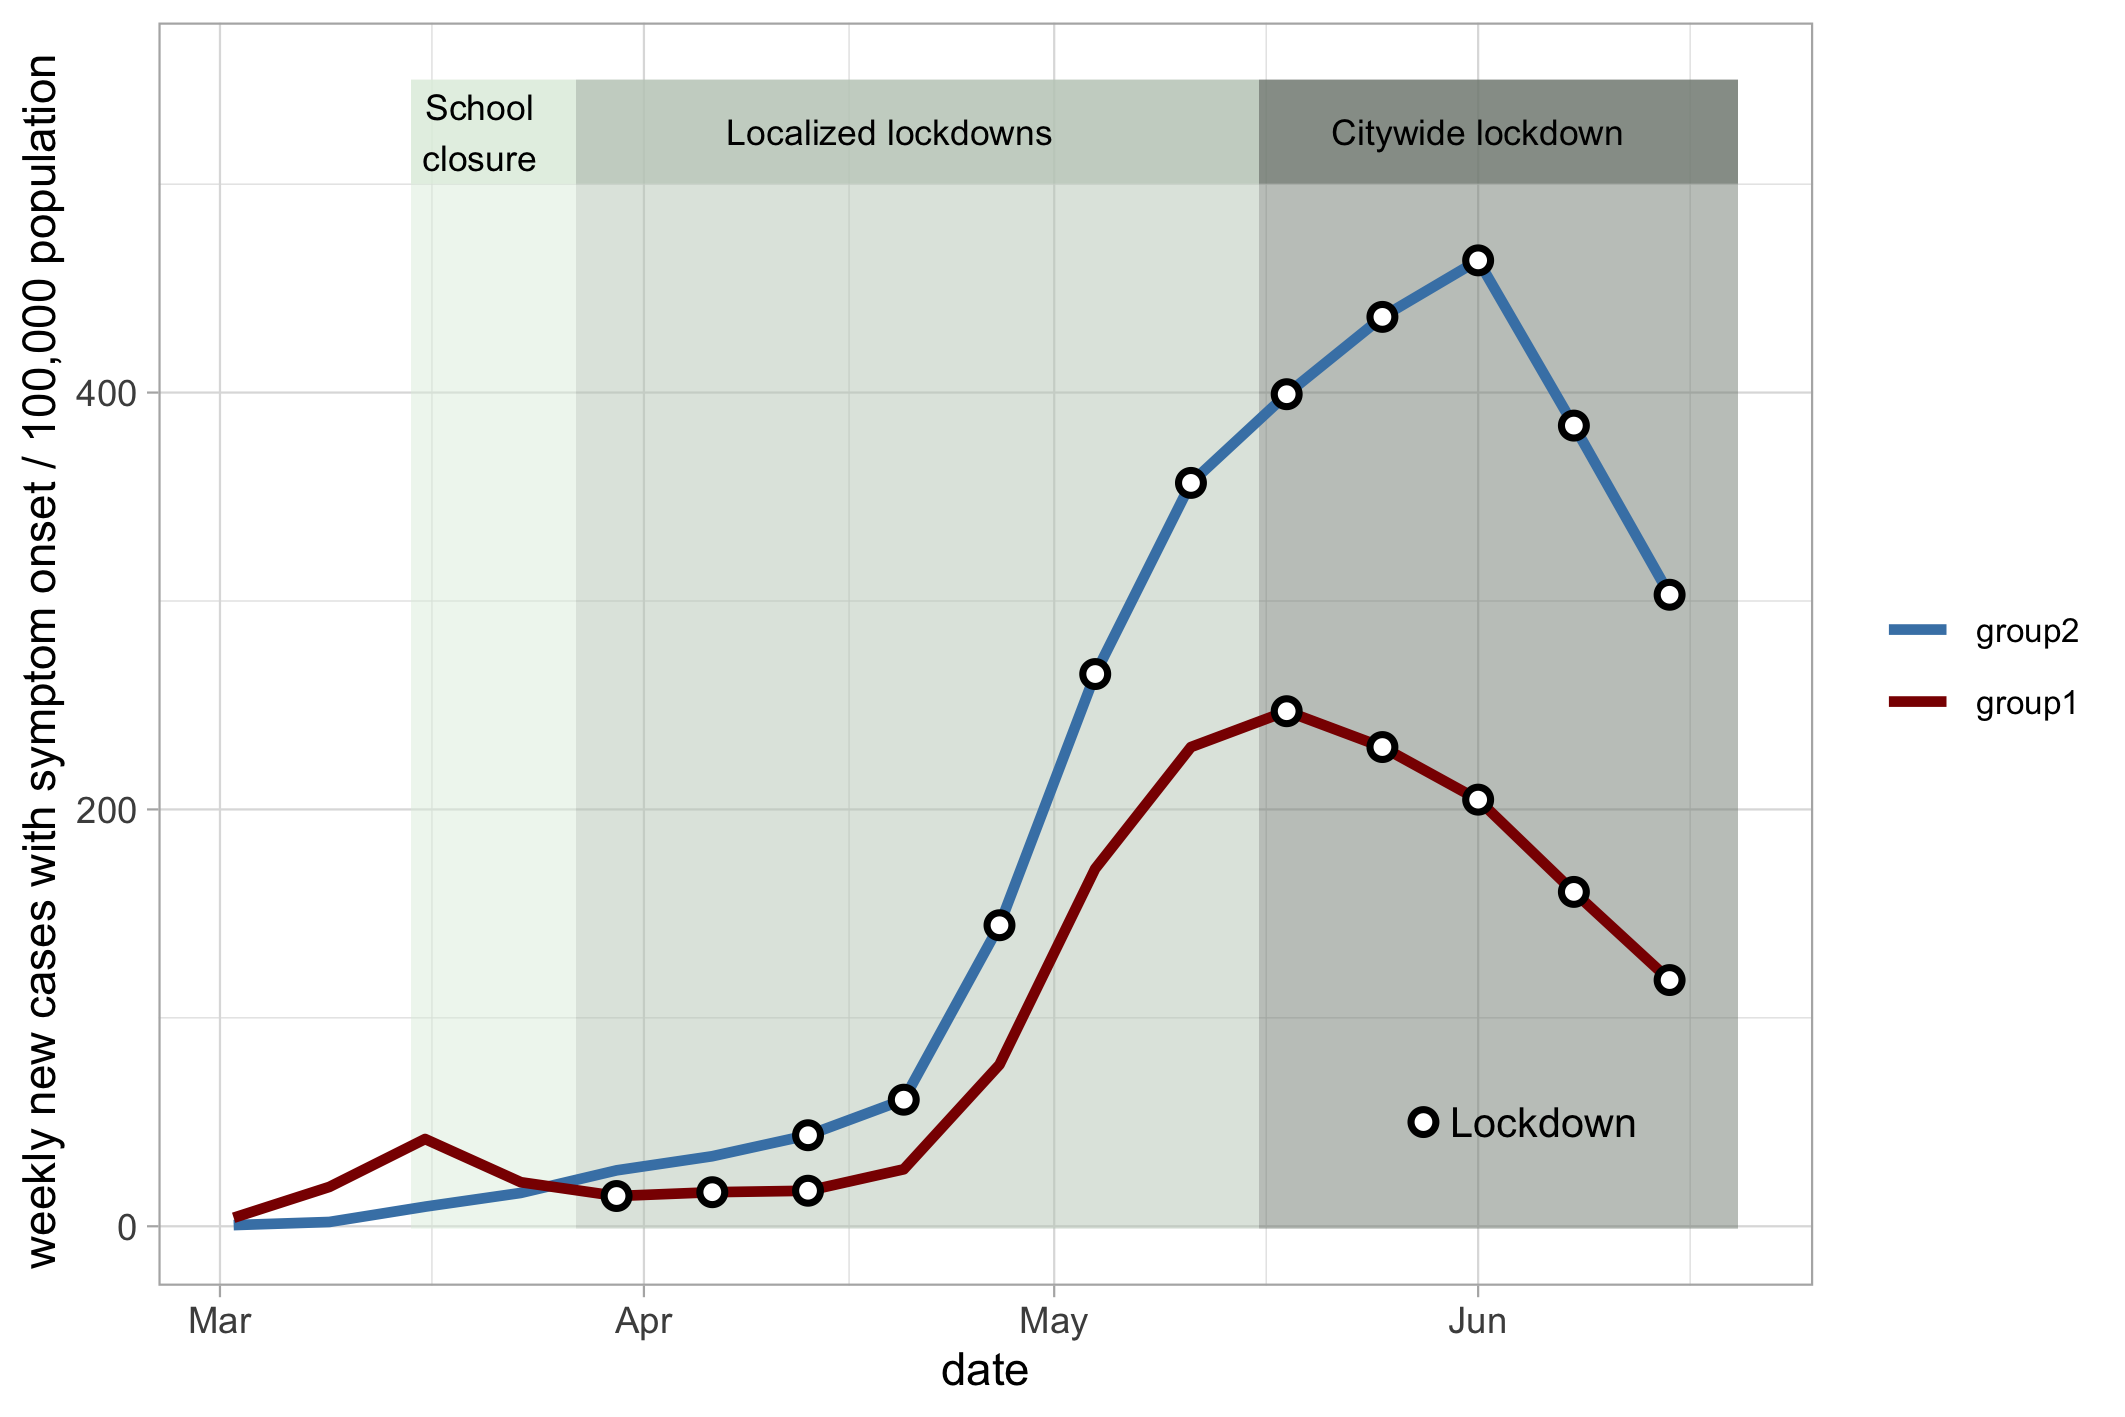
\includegraphics[width=0.7\textwidth]{imagenes/figs_tabs_pandemic/PNASFig1.png}
    \caption{New cases by week of symptom onset, grouped by areas where the first and second waves of localized lockdowns in Santiago were implemented.}
    \label{fig:cases_group}
\end{figure}

Why was it harder to contain the pandemic in group 2? %In fact, Further, there are important differences in shelter-in-place behavior between groups, with group 1 reducing its mobility almost 75\% more than group 2. 
Our work aims to understand how voluntary shelter-in-place behavior and compliance to lockdowns may vary substantially depending on the characteristics of the population in a city. 
In fact, there are important differences in shelter-in-place behavior between groups, with group 1 reducing its mobility significantly more than group 2. 
Furthermore, it is in fact revealing that 61\% of the total population in group 1 belongs to the highest-income segment. This is in part because the pandemic was mostly initiated by foreign travelers and the initial outbreak was concentrated in the higher-income areas. By contrast, only 2.5\% of group 2 belongs to the  highest-income segment. More generally, in developing countries like Chile there is typically high heterogeneity in socioeconomic and educational levels within cities.\footnote{The Metropolitan Region that includes the city of Santiago has a Gini index of 0.5, the largest in the country, and exhibits not only important income inequalities, but also high levels of educational and urban segregation \citep{romero2012assessing, elacqua2012impact}.} 

%\gw{[Should we also include mobility of groups 1 and 2?]}\mgoic{En el periodo group 1 tiene una reducción de movilidad de 0.384, mientras que el grupo 2 tiene una reducción de 0.220 con lo que digo que la reducción de uno con respecto el otro es casi 75\% (0.384/0.220-1)=0.743. Está dificil meter el número en el párrafo. Revisar si fluye.}

This analysis provides evidence that the interaction between mobility and socioeconomic status is important for understanding the spread of the pandemic. In this study we show how people's socioeconomic level has a significant impact on people's response to voluntary shelter-in-place directives and lockdowns, the most widely used non-pharmaceutical interventions in the Covid-19 pandemic.
A distinctive feature of our study is that we consider granular location data to characterize how mitigation measures reduce the population's mobility and estimate how these reductions contain the rate of infection. More specifically, to study mobility we collected detailed data from the usage of the wireless telecommunications infrastructure to build localized measures of mobility, capturing shelter-in-place adherence and population flows between local areas. 

While other studies also use mobility data to study the effect of lockdowns, our approach is novel in terms of specifically measuring trips and shelter-in-place behavior within a specific city. This is in contrast to capturing heterogeneous behavior also with respect to income but across an entire country such as the U.S. \citep{weill2020social}. Also at the level of the U.S., \cite{chiou2020social} explores the role of not just income but also internet access in adherence to shelter-in-place directives. In addition, \cite{valentino2020location} makes a model-free comparison of mobility between the wealthiest and the poorest areas in several metropolitan areas in the U.S. Finally, \cite{bonaccorsi2020economic} uses Facebook data to analyze the impact of lockdowns on mobility in Italy.
%The paper by Chiouw and Tucker is highly relevant and we now cite in our paper. Thanks for the pointer. The paper uses Safegraph data to show that both high income and unequal diffusion of high-speed Internet are key determinants of compliance  with state-at-home directives in the United States. As the authors acknowledge, the paper has some limitations that we think our paper addresses, and therefore, we believe our work provides an important contribution to the literature. The work by Chiouw and Tucker uses data from February and March and only from the United States. Instead, we use data all the way through July and from a developing country, Chile, complementing their work and other papers that use US data only. In this sense, a distinctive feature of our study is that we study shelter-at-home behavior in a large city of a developing a country. Further, our mobility data is more granular than the Safegraph data and allow us to measure trips within the city, which we now capture on the new measure described above, $MobRisk$. Similar comments apply to the  NYT article that uses data from a different company, Cuebiq, also focusing on US cities on February and March. In addition, we added several new relevant references
In contrast to these studies, our measures of lockdown compliance are localized, measuring mobility in geographic units of 2,000--3,000 people, which provides a sample size of more than 1,600 zones in the city of Santiago during a four-month period. This level of granularity within a city allows us to determine not only whether people leave their residences, but also whether they are traveling to riskier areas of the city and are more likely to interact with the infected population. Building these risk-adjusted mobility measures is an important contribution of our work. 
 
In more detail, our first main contribution is a detailed analysis to identify the causal effects of lockdowns and voluntary shelter-in-place directives on mobility and how these effects are moderated by demographics. Our identification strategy takes advantage of the localized implementation of lockdowns and the heterogeneity of the demographic characteristics across the city. This analysis with panel data reveals that socioeconomic characteristics are key in determining voluntary shelter-in-place behavior and lockdown compliance.
Our estimates indicate that while zones of high socioeconomic levels can exhibit reductions in mobility of around 50\% to 90\% depending on the specific mobility metric used, these reductions are only 20\% to 50\% for lower-income communities. The large reductions in higher-income communities are significantly driven by voluntary shelter-in-place behavior.
%60-80\% (significantly driven by voluntary shelter-in-place behavior), lower income zones only reduce mobility by 20-40\%. 
These differences that we found for Santiago, a metropolitan city in a developing country, are comparable in magnitude to those reported in previous work across an entire developed country \citep{weill2020social}. 

Using panel data methods, we then show that these constructs of mobility are an important predictor of outbreaks at the municipality level. We show that a 67\% reduction in mobility -- which is about the difference in mobility observed between high- and low-income municipalities  -- correlates with a 36\% reduction in the rate of infection (an elasticity of 0.5 approximately).  This result contributes to the study of the impact of non-pharmaceutical interventions on epidemiological outcomes \citep{flaxman2020estimating,villas2020we,fang2020human,allcott2020economic}. 

Our work is closely related to \cite{cuadrado2020impact}, which studies the impact of lockdowns on mobility and infections in specific regions of Chile. Unlike their work, our study focuses on a single city (Santiago) that was subject to localized lockdowns, using a more granular analysis to identify the moderating effect of demographics on the response to lockdowns and voluntary shelter-in-place directives. Our work is also related to \cite{bennett2021all},  which uses a synthetic control method to analyze the impact of lockdowns in the city of Santiago, showing that socioeconomic conditions influence their effect on the rate of infection significantly. Whereas in that study the focus is on the heterogeneous impact of lockdowns on infections, our work is focused in identifying mobility as the main underlying mechanism;  in this sense, these two studies are complementary. 
%Overall,  a novel contribution of our work is providing a granular analysis of the impact of shelter-in-place policies on mobility in a large city of a developing country. 

Our results show that  failing to acknowledge the heterogeneous effect of voluntary shelter-in-place directives and lockdowns can have dramatic consequences in the containment of the pandemic. It also confirms the challenges of reducing mobility in lower-income communities, where people generate their income from their daily work and cannot work remotely. Finally, our results suggest that, to be effective, shelter-in-place restrictions in municipalities of low socioeconomic levels might have to be complemented by other measures that induce their inhabitants to increase compliance. Given that these communities do not have easy access to basic services, it seems fundamental to provide aid to cover basic needs.
 
Some of the results of this study were made publicly available during the first weeks of the citywide lockdowns, receiving substantial attention from the public press and government authorities, underscoring the importance of reducing mobility to control the pandemic and of providing aid to low-income families to help them adhere to the lockdown and shelter-in-place requirements.\footnote{Please refer to https://isci.cl/tag/geointeligencia/.}
% \footnote{We published several mobility reports that were made available to the public. They had, and still have, a large impact on decision makers and on the media, with more that 70 appearances on newspapers, radio and TV (see \href{https://isci.cl/tag/geointeligencia/}{[URL 1]}, \href{https://www.elmostrador.cl/dia/2020/05/30/estudio-revela-alta-movilidad-en-comunas-de-menores-ingresos-durante-cuarentena-en-la-rm/}{[URL 2]}, \href{https://www.emol.com/noticias/Nacional/2020/05/29/987542/Estudio-movilidad-RM-comunas-ingresos.html}{[URL 3]}, \href{https://www.cnnchile.com/coronavirus/estudio-isci-movilidad-cuarentena-comunas-pobres_20200529/}{[URL 4]}, \href{https://www.emol.com/noticias/Nacional/2020/06/03/988029/Gran-Santiago-cuarentena-movilidad-30.html}{[URL 5]}, \href{https://twitter.com/acouvecorrea/status/1268980599748001792?s=20}{[URL 6]}).}


\section{Data and measures of mobility}

This study uses four different data sources for Santiago, Chile: (i) Covid-19 infections, (ii) dates of government-imposed lockdowns, (iii) demographic information, and (iv) mobility data from mobile phones. For our analysis, we selected data from March 2 to July 3, 2020, in order to include data from points in time before the first case of Covid-19 was detected in Santiago, during partial lockdowns of the city, and during total lockdowns  of the city. In addition, we considered only the urban municipalities of Santiago, which number 36 and together have a population of 6.1 million people. 

\subsection{Infections} 

Information on Covid-19 infections were  collected from the official public data made available by the Ministry of Health of Chile based on confirmed PCR tests (see \textit{Data Availability} in Appendix). We used data on the number of cases of infected individuals reported by date of initial symptoms (the only part of case counts that is self-reported is the date of symptom onset). The data is available weekly at the municipality level. Let $y_{\ell t}$ be the total number of infections in municipality $\ell$ in week $t$. In Appendix E we discuss a robustness analysis to check for underreporting of cases due to testing capacity and other factors.

\subsection{Mitigation measures} 

Information on the mitigation measures that were implemented in the city of Santiago was collected through press releases documenting the date of school closures and social distancing recommendations. Localized and citywide lockdowns were obtained from public data sources published by the Chilean Ministry of Science (see \textit{Data Availability}). These data are at the municipality level. Throughout the period, voluntary sheltering in place was strongly urged by the government and media.

\subsection{Demographics} 

Demographic information was collected from two different sources. The first source is the 2017 Chilean Census. This information is  available at the \emph{census unit} level and includes total population, elderly population (over 65 years), immigrant population, average household size, household density (average number of households per $km^{2}$), among other variables. For urban areas, the census unit corresponds to a city \emph{block}, which is the minimum aggregation unit we observe for Santiago. 

The second source of demographic information is a public data set from 2012, which provides the predominant socioeconomic group (SEG) at the block level. SEGs are based on income, education, and employment of the head of household \citep{meier2004social}. Following a common practice in other studies  \citep{romero2012assessing, hernandez2018twelve}, we grouped SEGs into three categories: high, medium, and low socioeconomic groups (HighSEG, MedSEG, and LowSEG, respectively). These demographics were aggregated to the census zone level. Each census zone is composed of several census blocks and has an average population of 3,661. The city of Santiago has 1,864 census zones, with 1,639 of them contained within the urban municipalities. Using principal component and cluster analysis we show that the socioeconomic classification defined above (HighSEG, MedSEG, and LowSEG) is highly correlated with all other demographic indicators (see Appendix A for details). Hence, for the econometric analysis we use these socioeconomic groups as our main variables of demographics. %( \textit{SI} further validates this using a principal component and clustering analysis).

\subsection{Mobility data} \label{sec:mobility}

Mobility data was collected via anonymized mobile phone usage, georeferenced by triangulation of antenna connections \citep{drane1998positioning}. Although other studies have also used measures of mobility based on mobile phone usage (e.g, \cite{GoogleMobilityReport, SafeGraph}), for this study we developed new  measures capturing both origins and destinations of mobility patterns in the city. These are specifically designed to measure shelter-in-place behavior, compliance with lockdowns, as well as population movements throughout the city.

Each mobile phone is associated with a \textit{home zone}, defined as the census zone in which the device is most frequently observed between 9--11pm during the month of observation. To prevent spurious associations with home zones, in the process we considered only users with a minimum of five observations in that location during the month. On average, in each census zone we observe 53 devices per every 100 inhabitants. Considering that there is an estimated 1.35 devices per capita, our sample seems to be quite large, capturing on average more than a third of the devices, while the rest would be from different providers. Furthermore, since the value proposition of different providers is quite similar we believe our sample of mobile phones is representative of the population. There is little product differentiation in the market and based on our exploration of the data, the participation of our mobile provider was slightly larger for higher socioeconomic groups. Hence, if any bias exists, it would lean towards underestimating the difference in mobility between high- and
low-income zones (since we are likely to over sample the relatively higher-income population from the low-income zones).

%On average, in each census zone we observe 53 devices per every 100 inhabitants.  Considering there is a high penetration of mobile technologies in Chile with an estimated of 1.35 devices per capita, is very likely that users that we do not observe in the sample also have a cell phone, but from a different provider. The value proposition of different providers is quite similar. \newgw{Hence, overall, we believe our sample of mobile phones is representative of the population. There is small product differentiation in the market and based on our exploration of the data, the participation of our mobile provider is slightly larger for higher socioeconomic groups. Hence, if any bias exists, we may be underestimating the difference in mobility between high- and low-income zones.}

To measure mobility, the location of each (anonymous) device was tracked on each day during two non-overlapping time intervals: AM (10am--1pm) and PM (2--5pm). These time intervals were chosen to capture work-commuting patterns and, consequently, the sample excludes weekends and holidays.  For each time interval on each day, every observed device is assigned to  a \textit{destination zone} defined as the census zone in which the device is most frequently observed. This information gives us an anonymized description of the mobility of the population. 

\subsection{Mobility measures} \label{sec:mob_meas}

The information about movements of devices from their home zone to other zones in the city provides an origin-destination matrix that is constructed as follows.  Define $\hat f^b_{ijd}$ as the number of devices from home zone $i$ that traveled to destination zone $j$ during the time interval $b\in\{AM,PM\}$ on day $d$.\footnote{The sum $\sum_j \hat f^b_{ijd}$ represents the number of devices from home zone $i$ that were observed in each day and interval.} Then, the weekly average number of devices from home zone $i$ observed in destination zone $j$ in week $t$ in each time interval $b$, $f_{ijt}^b$, is calculated as the mean of the daily values excluding weekends and holidays in this aggregate. Furthermore, to have a conservative measure that avoids double-counting of individuals that may appear in both time intervals, we extract a single weekly matrix by taking the entry-wise maximum between both matrices, $f_{ijt}=\max\{f_{ijt}^{AM}, f_{ijt}^{PM}\}$. For robustness, we also study a specification considering the sum of $f_{ijt}^{AM}$ and $f_{ijt}^{PM}$, that is, $f_{ijt}=f_{ijt}^{AM} + f_{ijt}^{PM}$ (see Appendix E). The results obtained from both specifications are similar. % \gw{Make sure all results with sum are in App and confirm results are similar. Also explain both specifications.} %Note that taking max/  and then average is in between the two}

Under the assumption that the sample of devices is a representative sample of the population, the measure $f_{ijt}$ is a proxy for the weekly average number of people who leave their home zone $i$ for destination zone $j$ in week $t$. Using this information, we calculate measures of outward mobility in each zone:
\begin{align}
  \bar f_{ijt}=\frac{f_{ijt}}{\sum_{j}f_{ijt}}
 \quad & \mbox{and} \quad
MobOut_{it} =\sum_{j:j\neq i} \bar f_{ijt} %\label{eq:FracOut}
\end{align}
Thus, $\bar f_{ijt}$ is a proxy for the fraction of the weekly average number of people with residences in zone $i$ who travel to zone $j$ in week $t$, while $MobOut_{it}$ is a proxy for the fraction of the weekly average number of people with residences in zone $i$ who leave that zone in week $t$. 

While the analysis of the impact of lockdowns on mobility is done at a granular census zone level, to conduct the analysis of the effect of mobility on infections, we aggregate this zone-level mobility measure to the municipality level via a population-weighted aggregation. This is because municipalities are the most granular units for which infection data is available. With some abuse of notation we define the counterpart of $MobOut_{it}$, but at the municipality level, as
\begin{align}
 MobOut_{kt}%=\frac{\sum_{i:c(i)=k}Pop_i\cdot MobOut_{it}}{\sum_{i:c(i)=k}Pop_i} 
=\frac{\sum_{i:c(i)=k}\sum_{j:j\neq i}Pop_i\cdot \bar f_{ijt}}{\sum_{i:c(i)=k}Pop_i}\ , \label{eq:MobOut}
\end{align}
where $c(i)$ denotes the municipality containing census zone $i$ and $Pop_i$ denotes the population size of census zone $i$. This measure corresponds to the proportion of the population of municipality $k$ that leaves its home zone, and so provides an aggregated measure of outward mobility.\footnote{The data reveals that the number of mobile phones observed in each home zone typically decreases with time in our sample. One potential explanation is that devices used at home use WiFi connections more frequently, reducing the amount of cellular data and thereby making these devices less likely to appear in the sample. Ignoring this effect may lead to underestimating shelter-in-place compliance. Hence, we developed a correction that we also use in some of our analysis, explained in Appendix E.}
%Note that this is the $NormOut$ variable, but not normalized by the baseline.

%\delgw{We also normalize with respect to a baseline period $\mathcal{T}_b=\{9,10\}$, which corresponds to March 2--13, which were the first weeks of the epidemic in Chile, when it was still confined to a few cases and mobility had minimal variation.Hence, for municipality $k$ and week $t$, we define the following municipality-level measure of normalized mobility:
%\begin{align}   NormOut_{kt}=\frac{\sum_{i:c(i)=k}Pop_i\cdot FracOut_{it}}{\sum_{i:c(i)=k}Pop_i\cdot FracOut_{i,base}} \label{eq:NormOut}\end{align}where $c(i)$ denotes the municipality containing census zone $i$, $Pop_i$ denotes the population size of census zone $i$, and $FracOut_{i,base}=\frac{1}{|\mathcal{T}_b|}\sum_{t\in{\mathcal{T}_b}} FracOut_{it}$ is the census zone mobility measure averaged over the baseline period.}

Finally, we define a more granular mobility measure that accounts for the infection load of different areas of the city, to capture risk of infection to which people are exposed when traveling across the city. To this end, following the same logic as \eqref{eq:MobOut},
we define a population-weighted outward mobility proportion from municipality $k$ to municipality $\ell$ in week $t$ as
\begin{align*}
    \tilde f_{k\ell t}=\frac{\sum_{i:c(i)=k}\sum_{j:c(j)=\ell, j\neq i}Pop_i\cdot \bar f_{ijt}}{\sum_{i:c(i)=k}Pop_i}.
\end{align*}
% \gw{Aldo: let's check consistency between $Mobout$ and  $\tilde f$ as sanity check.}
Recall that $y_{lt}$ is the total number of infections in municipality $\ell$ in week $t$ and $\sum_{\ell}  y_{\ell t}$ is the total number of infections in the city. Based on this data, we define an infection-risk measure for municipality $m$ in week $t$, where we multiply by 100 to re-scale the risk metric appropriately: 
\begin{align*}
     Risk_{mt}=100\cdot\frac{\sum_{\ell}\tilde f_{\ell mt}\cdot y_{\ell t}}{\sum_{\ell}y_{\ell t}} ,
\end{align*}
which represents the proportion of infected individuals in the city that enter municipality $m$ in week $t$. This is used to construct a risk-weighted mobility measure for municipality $k$ in week $t$:
\begin{align*}
    MobRisk_{kt}=\sum_{m}\tilde f_{kmt}\times Risk_{mt}  % \ ,\label{eq:mobrisk_mun}
\end{align*}
which is a proxy for the risk that an individual from municipality $k$ will be exposed to an infected individual when traveling across the city. \textit{MobRisk} weights the outflows of the focal municipality ($k$) with the risk of the destination municipality ($m$), and sums over all municipalities, thereby accounting for the externality generated by the mobility of potentially infected people across the city.

Similarly, we define a measure of mobility risk at the census zone level. Let
$\hat f_{i\ell t}=\sum_{j:c(j)=\ell, j\neq i}\bar f_{ijt} \ ,$ which is a proxy for the fraction of the weekly average number of people with homes in zone $i$ who travel to municipality  $\ell$ in week $t$. This is used to construct a risk-weighted mobility measure for each census zone (with some abuse of notation):
$
    MobRisk_{it}=\sum_{m}\hat f_{imt}\times Risk_{mt}.  
$

In Appendix D we validate our measures and in Appendix E we also consider alternative measures of mobility using data from the integrated public transport system of Santiago.

\subsection{Descriptive analysis of mobility}

The left panel of Figure~\ref{fig:Temporal_evolution_of_mobility} shows the temporal evolution of $MobOut_{kt}$ for different municipalities of Santiago that 
represent different socioeconomic strata. The measure is normalized with respect to a baseline period that  corresponds to March 2--13, which were the first weeks of the epidemic in Chile, when it was still confined to a few cases and mobility had minimal variation. The points mark weeks where the municipality had more than half of its population under lockdown.\footnote{By construction, the first weeks taken as a baseline have essentially zero variation.}
From the week of March 16 we begin to observe a marked decrease in mobility; this date coincides with the closing of schools in Chile. Despite the fact that the schools closed concurrently throughout the city of Santiago, the effect of voluntary shelter-in-place behavior is very heterogeneous. For higher-income municipalities such as Las Condes, mobility decreased by 30\% and the following week by 40\%. By contrast, the effects on mobility were between 10\% and 20\% for lower-income districts such as Puente Alto, and even less for El Bosque. The effects for the municipalities of Santiago and Ñuñoa are somewhere in between.\footnote{We note that the fraction of HighSEG in Las Condes is 67\%, while for Ñuñoa is only 28\%.}  
\textbf{\begin{figure}[htb]
    \centering
    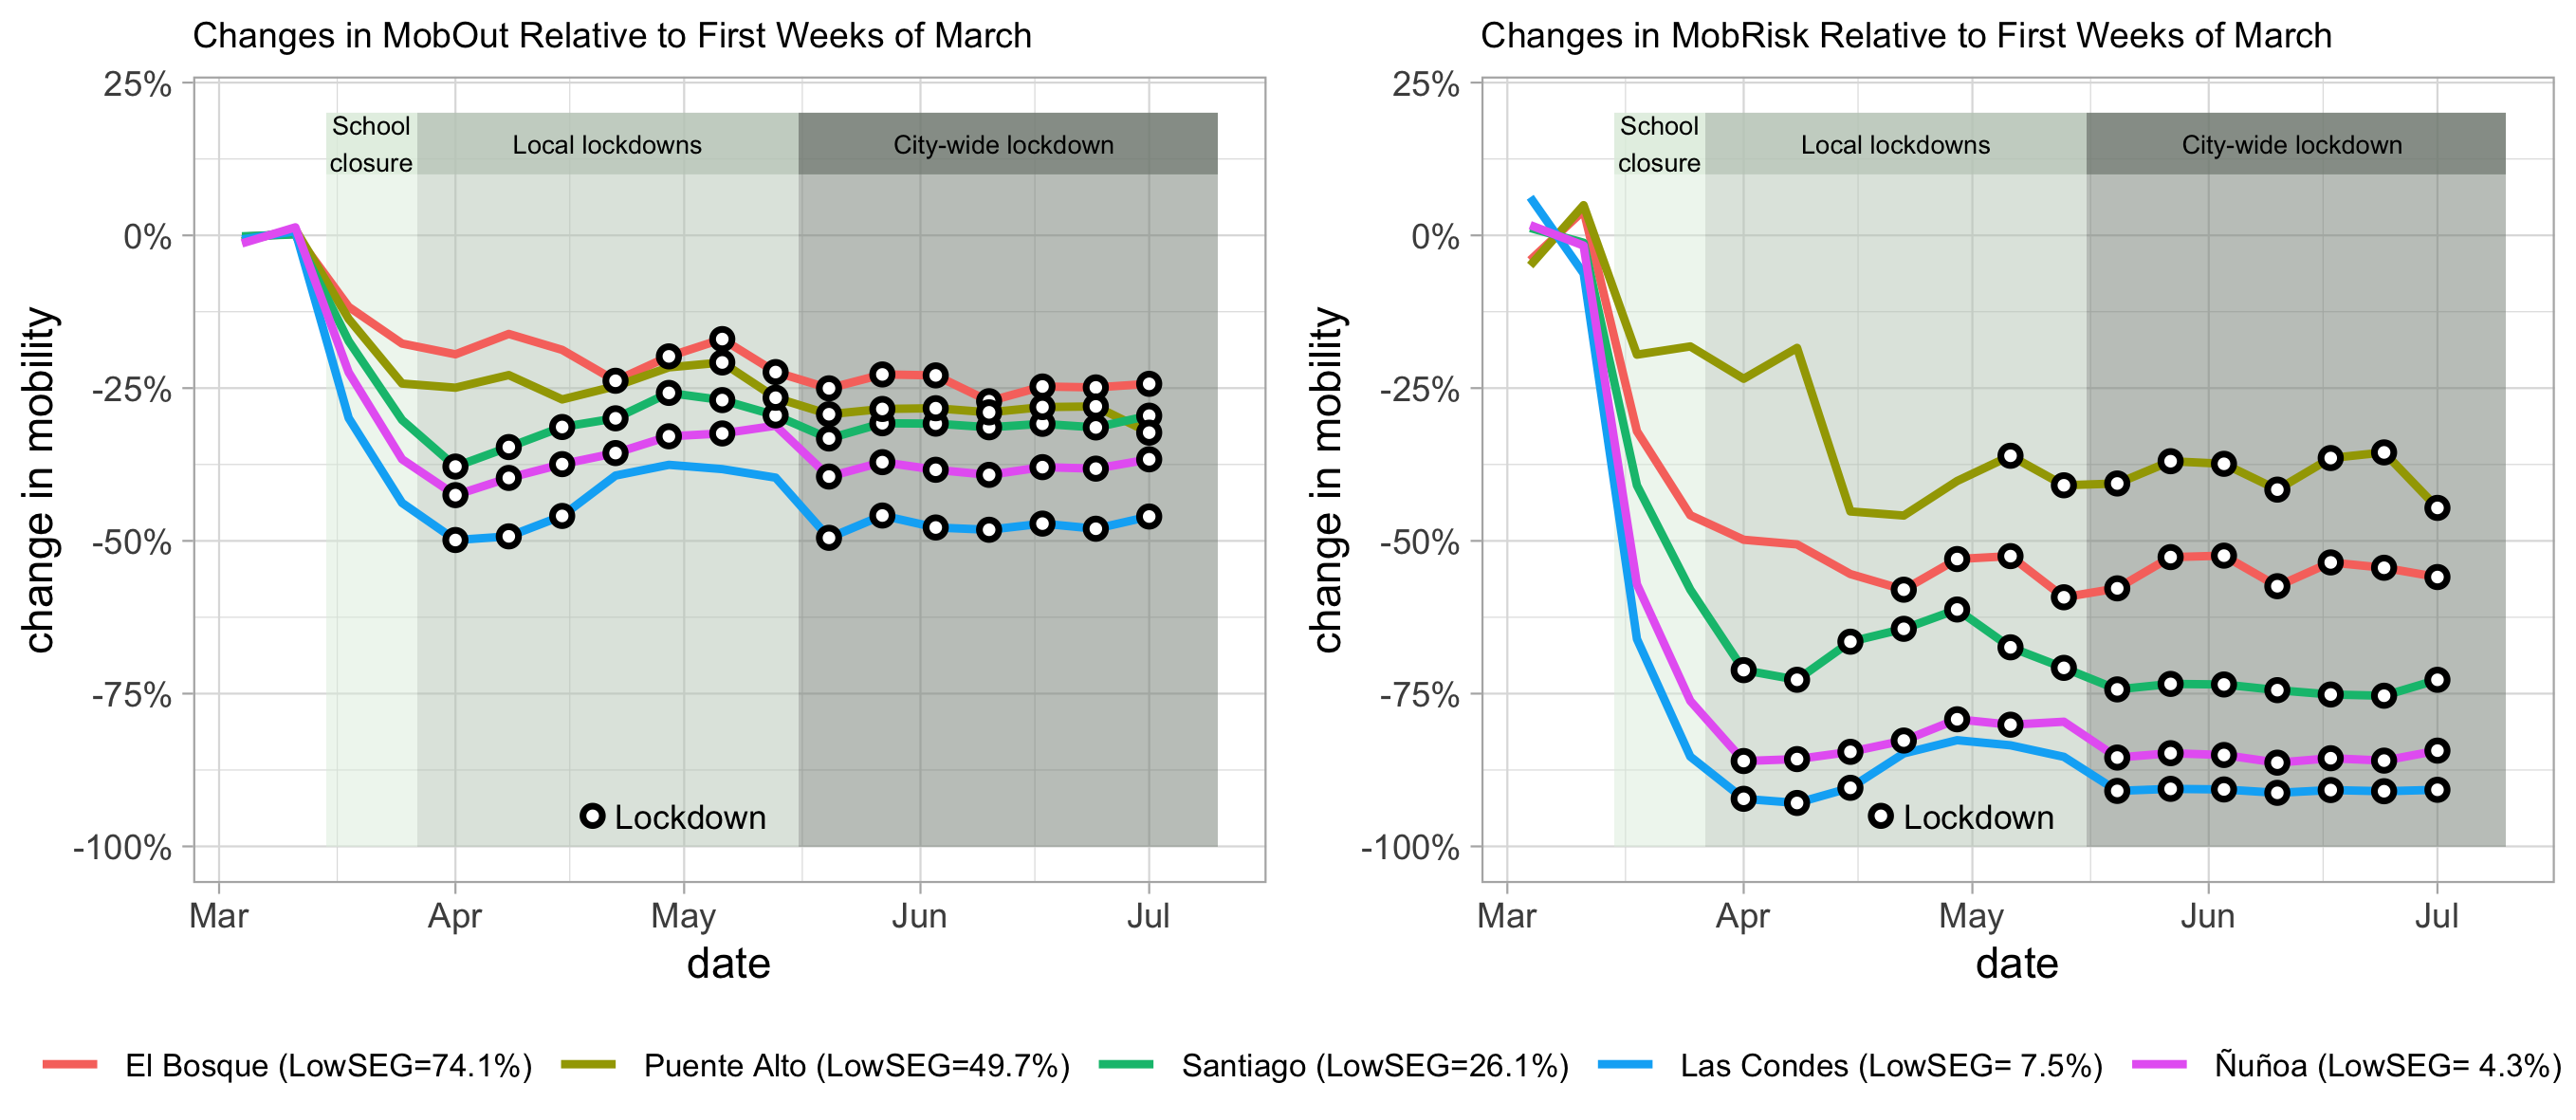
\includegraphics[width=\textwidth]{imagenes/figs_tabs_pandemic/Fig2_v1_both_2.png}
    \caption{Temporal evolution of mobility in different municipalities of Santiago, measured as fraction of total trips leaving home zones relative to the baseline period (March 2--13). Legend shows in parentheses the fraction of population in the low socioeconomic segment (LowSEG) for each municipality.}
    \label{fig:Temporal_evolution_of_mobility}
\end{figure}}

Then, on March 27, mandatory lockdowns were initiated in the municipalities of Santiago, Ñuñoa, and Las Condes (as well as other municipalities; these correspond to group 1 in Fig. \ref{fig:cases_group}). Although this reduced mobility by an additional 5 to 8 percentage points in these municipalities, the decrease is relatively small compared to that recorded before the imposition of mandatory lockdowns.
In the last two weeks of April, the higher-income municipalities were released from mandatory lockdown, while  lockdowns were imposed on Puente Alto and El Bosque (as well as other municipalities; these correspond to group 2 in Fig. \ref{fig:cases_group}). In these latter cases, we do not observe a significant effect in the reduction of mobility associated with mandatory lockdowns. Indeed, Figure \ref{fig:Temporal_evolution_of_mobility} illustrates that in the last few weeks of April mobility in higher-income municipalities -- which were no longer under lockdown -- remained well below that of the others that were under mandatory lockdowns.\footnote{These patterns are consistent with results presented in other reports that used data from another mobile phone company and differently constructed mobility measures \citep{IndiceMovilidadUDD}.} 
The differences in mobility between municipalities of different socioeconomic strata remain even as the entire city went into mandatory lockdown from mid-May through June. The mobility measure $MobRisk$ presents a similar evolution and heterogeneity across municipalities of different socioeconomic levels to $MobOut$, as presented in the right panel of Figure~\ref{fig:Temporal_evolution_of_mobility}. Table \ref{tab:summ_stats} shows summary statistics of these two mobility measures at the municipality level. (See also Appendix C for additional summary statistics at municipality and census zone levels).

% \newgw{1) Aldo: poner summ stats. Cambiar titulo graficos normalizados: Changes in Mobout/MobRisk Reltive to First Weeks of March }

\begin{table}[!htbp] \centering 
%   \caption{} 
%   \label{} 
\begin{tabular}{@{\extracolsep{5pt}}lccccccc} 
\\[-1.8ex]\hline 
\hline \\[-1.8ex]
Statistic & \multicolumn{1}{c}{N} & \multicolumn{1}{c}{Mean} & \multicolumn{1}{c}{St. Dev.} & \multicolumn{1}{c}{Min} & \multicolumn{1}{c}{Pctl(25)} & \multicolumn{1}{c}{Pctl(75)} & \multicolumn{1}{c}{Max} \\ 
\hline \\[-1.8ex] 
$MobOut$ & 411 & 0.529 & 0.064 & 0.326 & 0.508 & 0.572 & 0.721 \\ 
$MobRisk$ & 411 & 0.893 & 0.444 & 0.240 & 0.648 & 1.004 & 5.381 \\ 
% $FracLock$ & 411 & 0.164 & 0.330 & 0 & 0 & 0 & 1 \\
% $R$ & 411 & 1.297 & 0.678 & 0.559 & 0.822 & 1.549 & 4.000 \\ 
\hline \\[-1.8ex] 
\end{tabular}
\caption{Summary statistics of municipality-level mobility measures.}
\label{tab:summ_stats}
\end{table} 


In the next sections we present an econometric analysis confirming the patterns observed in Figures \ref{fig:cases_group} and \ref{fig:Temporal_evolution_of_mobility}. 
First, in Section \ref{sec:mobility} we show that after controlling for other possible factors, the main factor that explains the differences in mobility patterns between the municipalities in Santiago is indeed socioeconomic status. Then, in Section \ref{sec:infections} we show that mobility is in fact an important explanatory variable of infections. 

\section{The impact of socioeconomic level on mobility} \label{sec:mobility}

 In this section we explore the heterogeneous impact of shelter-in-place behavior and mandatory lockdowns on mobility and how they are moderated by socioeconomic level. 

%\subsection{Lockdown mitigation measures}

% The treatment effects of $Lockdown_{it}$ capture the zones where the localized interventions are actually implemented. However, lockdown interventions in a zone also generate externalities on other zones that commute from the focal zone and vice versa. For example, lockdowns establish closures on the workplaces of residents from other zones modifying commuting patterns. To capture this externality, we construct an additional measure that incorporates the effect on outflows to other zones. Define a \textit{baseline} flow percentage $b_{ij}$ from focal zone $i$ to another zone $j$ observed during the baseline period  $\mathcal{T}_b$:
% $$b_{ij} = \frac{1}{|\mathcal{T}_b|}\sum_{t\in \mathcal{T}_b}\frac{f_{ijt}}{\sum_{k:k\neq i} f_{ikt}},$$
% \newgw{where $\mathcal{T}_b$ corresponds to the ninth and tenth weeks of the year (March 2-March 13)}.
% Using the outflow $b_{ij}$ from the focal zone to weigh the impact of the lockdown on mobility, we compute a measure of the impact of lockdowns in other zones on the focal zone $i$ as:
% \begin{align}
% LockOther_{it} &= \sum_{j:j\neq i} b_{ij} \cdot Lockdown_{jt} \ .\notag %\label{eq:LockedOther}
% \end{align}

\subsection{Econometric model}

Our main model is a panel data linear regression model with cross-section $i$ defined by census zones analyzed in each week $t$, which fully exploits the cross-sectional variation at the most granular level. The model is estimated with the sample period from March 2 to July 3, 2020 (weeks 9 to 26 in the calendar year), in which the government implemented closing of schools, recommended sheltering-in-place, and adopted mandatory localized lockdowns and, later, a citywide lockdown in Santiago as explained above. To measure mobility we consider the two metrics we defined in Section \ref{sec:mob_meas}: \emph{MobOut}, which measures whether users leave their residences, and \emph{MobRisk}, which additionally measures whether users move to more risky areas. We use a log transformation that facilitates a relative interpretation of the coefficients and provides a better fit to the data. Thus, our main model to study mobility is defined as
%\begin{align}
%\log{(\text{Mobility}_{it})} &=\delta_{i}+\tau_{t} \cdot(\alpha D_{i}) + LockLocal_{it}\cdot(\beta D_{i}) + %u_{it} \label{eq:FracOut_wkhet}
%\end{align}
\begin{align}
\log{(\text{Mobility}_{it})} &=\delta_{i}+\sum_{s\in\mathcal{S}} \tau^s_{t} \cdot D^s_{i} +  \sum_{s\in\mathcal{S}} \beta^s D^s_{i}\cdot LockLocal_{it} + u_{it} \label{eq:FracOut_wkhet} \,
\end{align}
where $\mathcal{S}=\{$HighSEG$, $MedSEG$, $LowSEG$\}$. The parameters $\delta_{i}$ are zone fixed effects and we omit the constant in the regression. The covariates $D_i^s$ are continuous variables specifying the fraction of the population in zone $i$ that belongs to each socioeconomic group (note that $\sum_{s\in\mathcal{S}} D_i^s=1$). Hence, the week-SEG coefficients $\tau_t^s$ (which are multiplied by the fraction of the population in that SEG) capture citywide interventions and other exogenous shocks on a given week that could potentially have {\em heterogeneous effects across SEGs}. For example, these week-SEG coefficients of the first weeks (weeks 11 and 12) capture voluntary shelter-in-place behavior at the beginning of the pandemic before the imposition of mandatory lockdowns.  Further, the coefficients of week 20 capture mobility reductions associated with the citywide lockdown, which started that week. We omit the week-SEG coefficients for the first week of March, so that all the effects are measured with respect to this ``pre-pandemic'' week. The coefficients of $LockLocal_{it}$ together with the week-SEG coefficients $\tau_t^s$, all of which are estimated separately for the different socioeconomic levels, are the main treatment effects to be estimated in this model. 
 
The treatment variable \emph{LockLocal} captures the effect of {\em localized lockdowns}. We construct this variable to represent the fraction of days in week $t$ that census zone $i$ is under a localized lockdown. The staggered implementation of lockdowns across zones with different demographic characteristics provides an exogenous variation that allow us to identify the effect of these localized lockdowns and their heterogeneous effect across zones. As discussed above, the week-SEG coefficients  capture the effect of the citywide lockdown, and so we set  the variables $LockLocal$ equal to zero during the city's full lockdown. 

We also run a parsimonious model that fixes the treatment effect and week coefficients  to be homogeneous across zones (presented in Appendix F along with other alternative specifications and robustness checks). The qualitative findings of these complementary analyses are similar to those derived from the main models.

\subsection{Estimation results}

The main estimation results correspond to the weekly-SEG coefficients  and the variation in mobility due to localized lockdowns. We start discussing the results for the week-SEG coefficients. To facilitate visualization, we present the estimates for each socioeconomic group in Figure \ref{fig:weekEstrato.modelFullInteraction} (the table with the parameter estimates are included in Appendix F). Here, the three lines represent the percentage variation in mobility for hypothetical zones with 100\% of their population in the corresponding group. 

\begin{figure}[hbt]
    \centering
    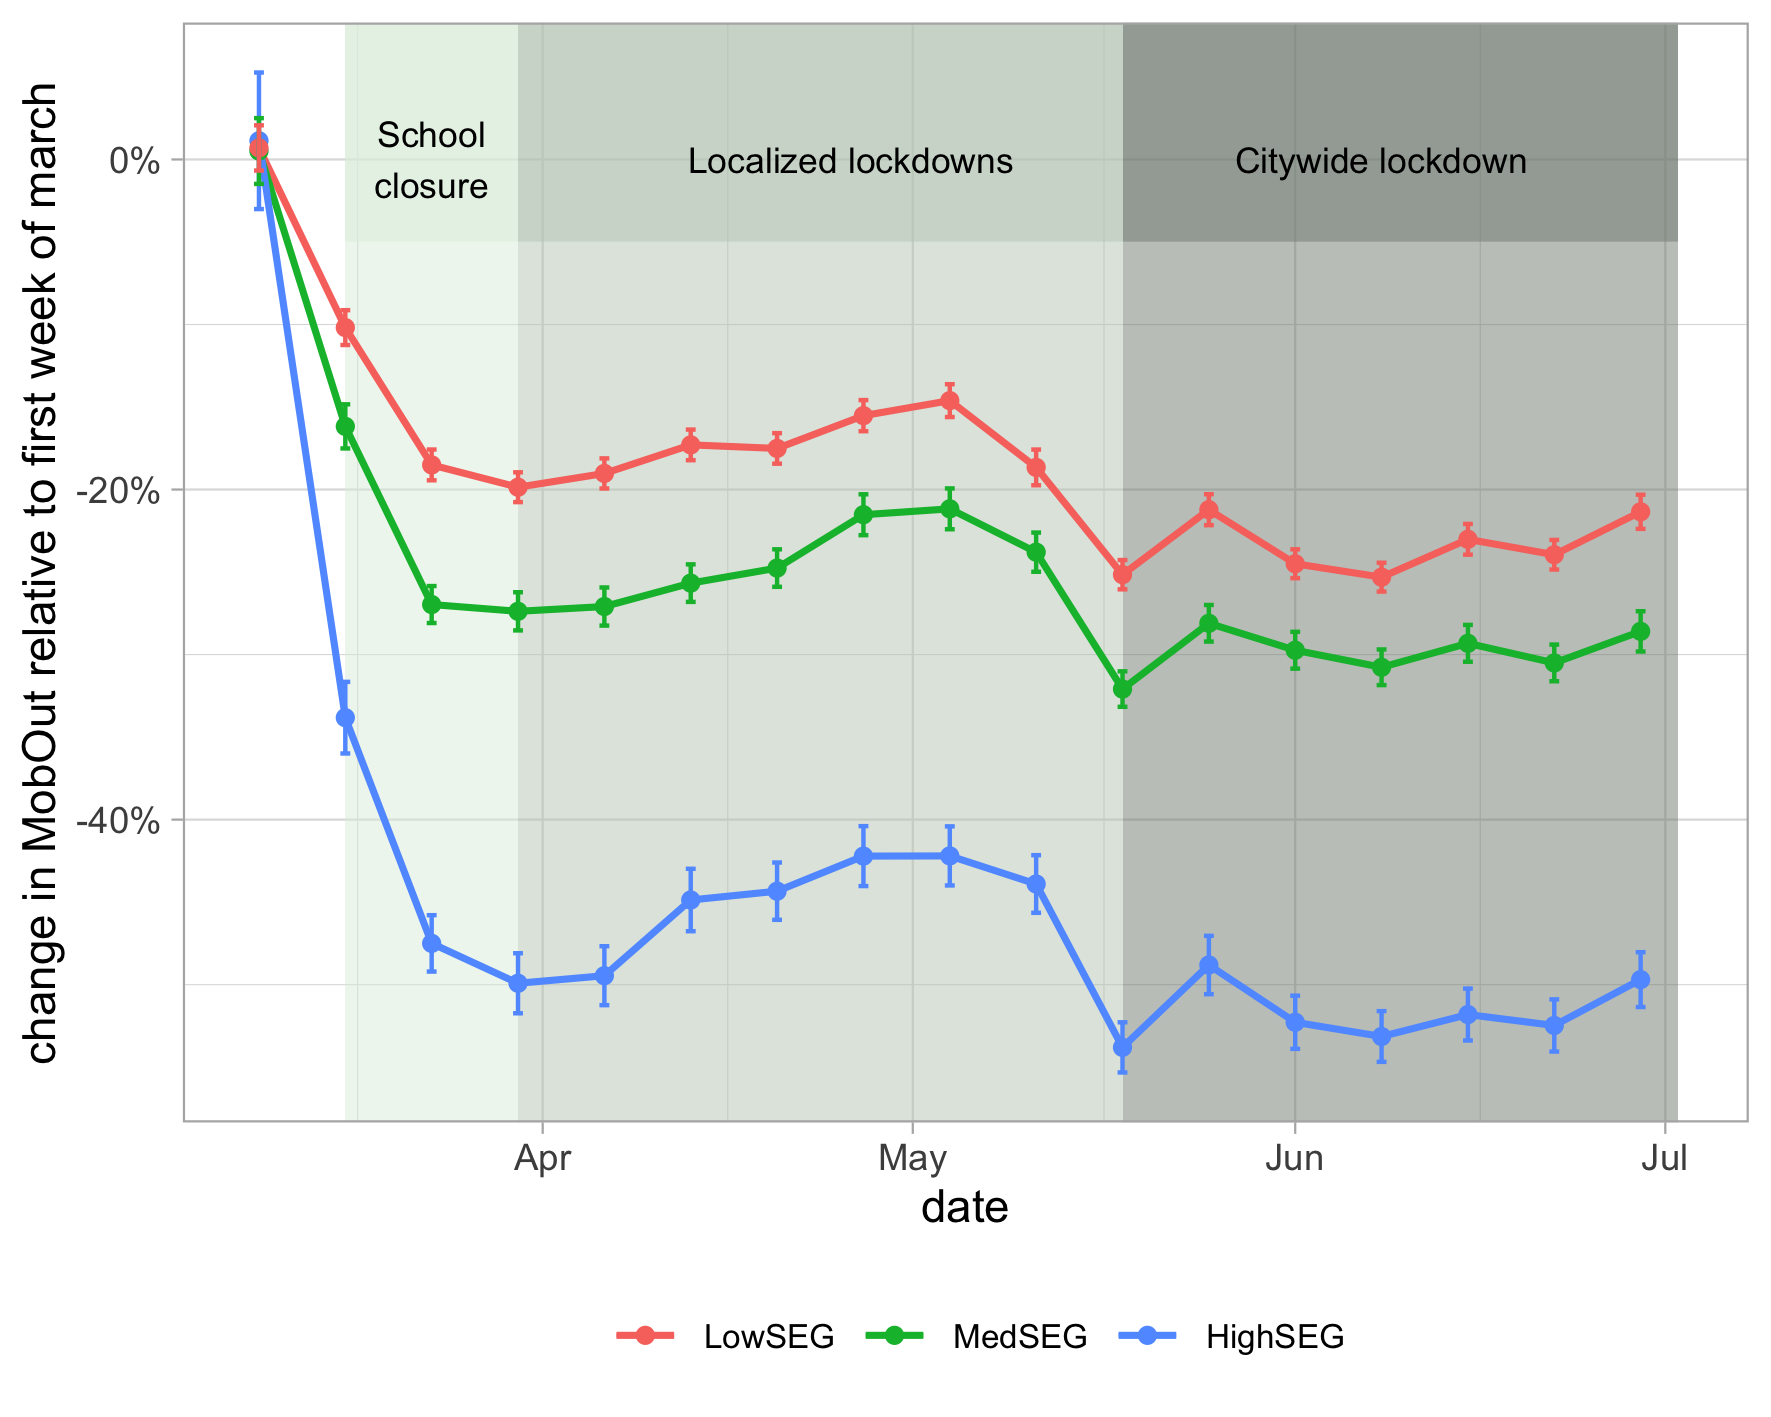
\includegraphics[width=.49\textwidth]{imagenes/figs_tabs_pandemic/LockdownOnMobility/PNASFig3_v4_LogFracOut_vcovHC_white1_HC1.png}
    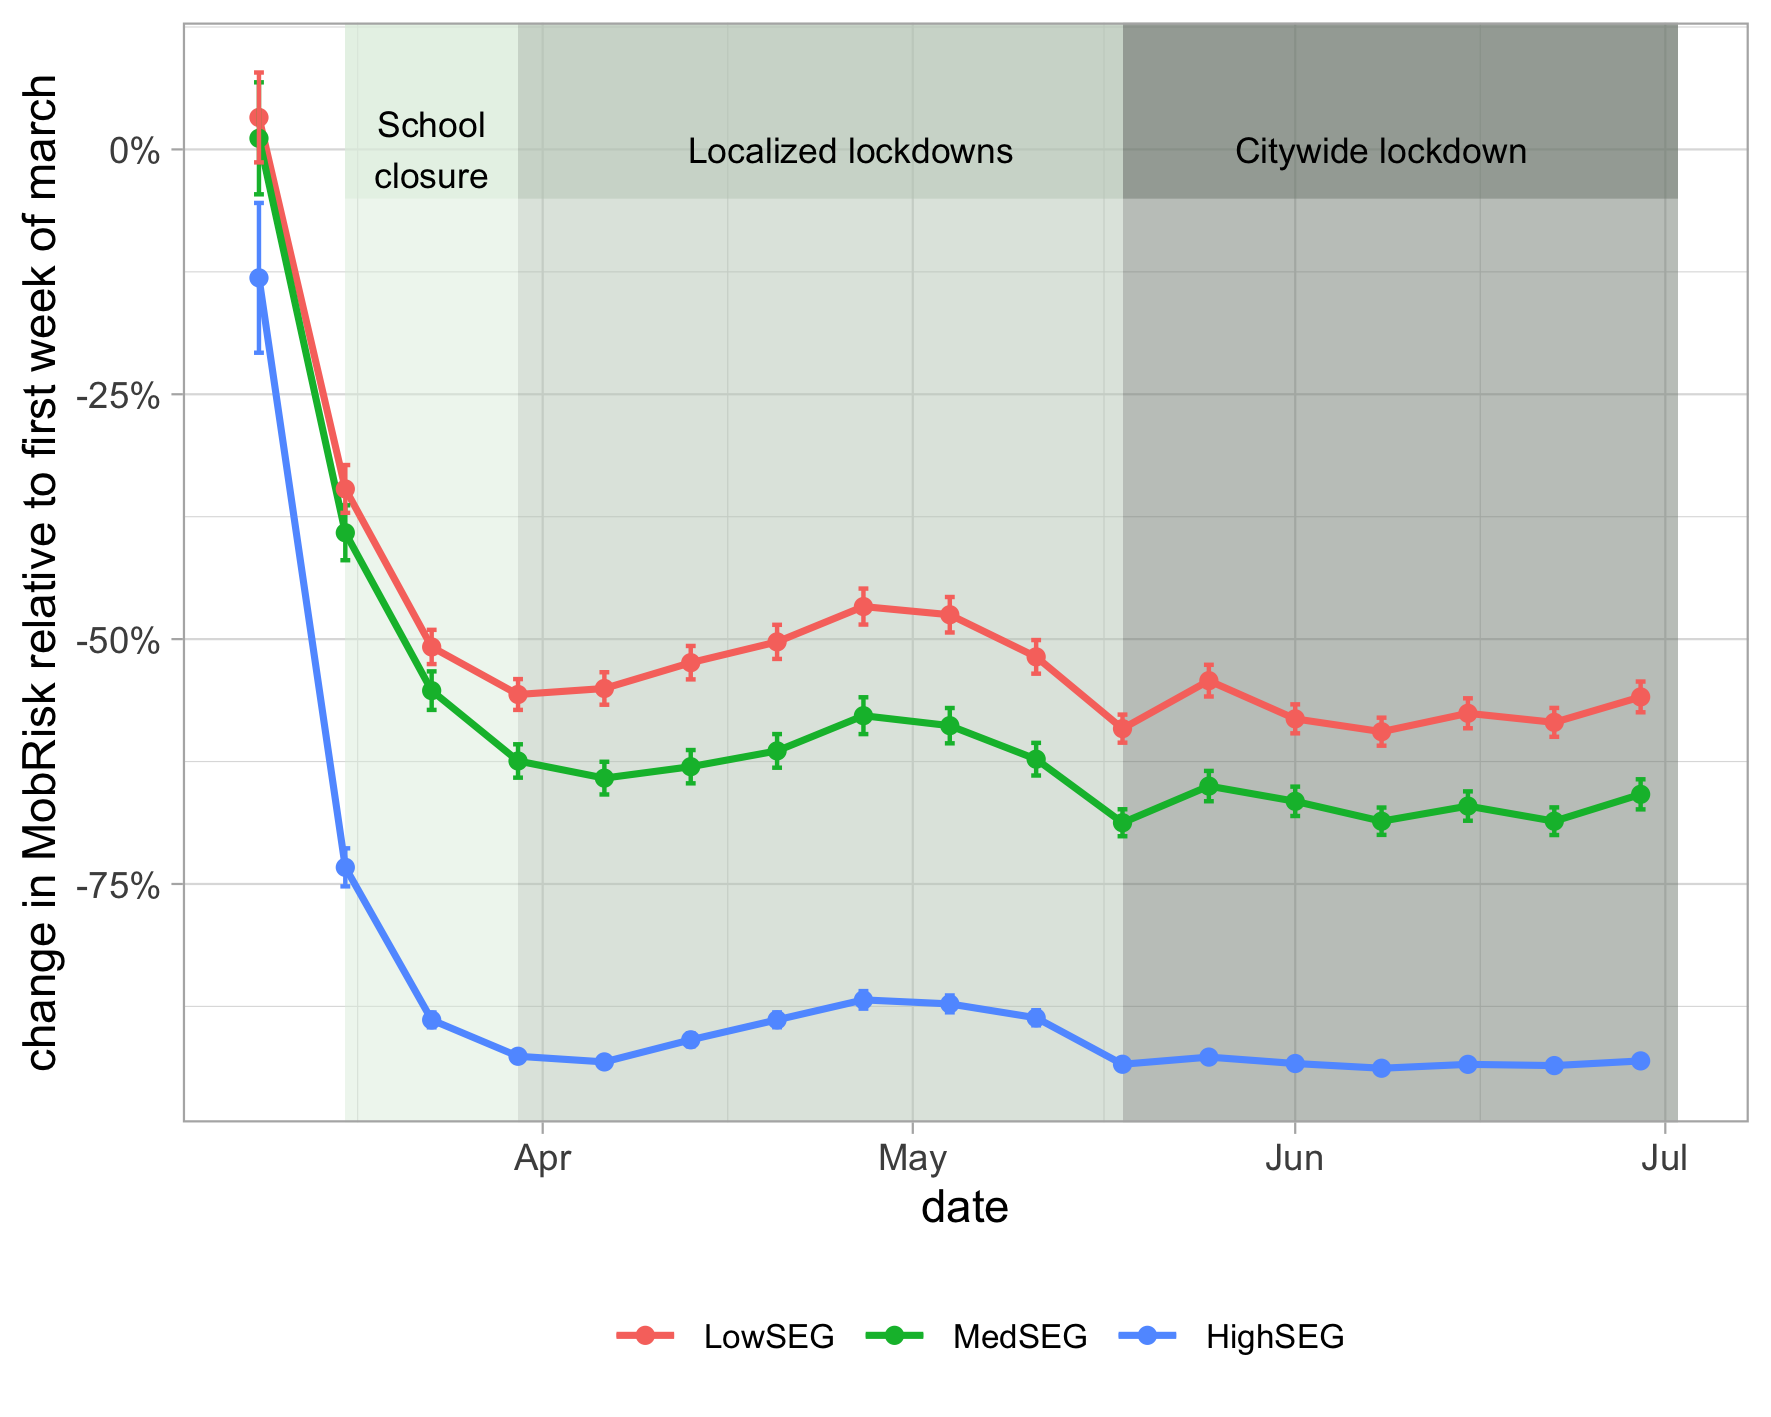
\includegraphics[width=.49\textwidth]{imagenes/figs_tabs_pandemic/LockdownOnMobility/PNASFig3_v4_LogMobRisk_vcovHC_white1_HC1.png}
    \caption{Week coefficients  interacted with socioeconomic group (week-SEG coefficients) for log(MobOut) and log(MobRisk) regressions. Error bars represent the 95\% confidence interval of the estimates (calculated using the Delta Method and robust standard errors).}
    \label{fig:weekEstrato.modelFullInteraction}
\end{figure}

% \begin{table}[htbp] \centering
%   \caption{Estimation results: Fraction leaving censal zone ($FracOut_{it}$).} Model \ref{eq:FracOut_wkhet} includes full interaction between week and the socio-economic factor, and interactions between the interventions and the socio-economic factors (separated into multiple columns).
%   \label{tab:results_mob} 
%   \footnotesize
%     %% Resultados analysis_mobility_v15_EL_week9-26.Rmd
\begin{tabular}{@{\extracolsep{-5pt}}lccccc} 
\\[-1.8ex]\hline 
\hline \\[-1.8ex] 
 & \multicolumn{5}{c}{\textit{Dependent variable:}} \\ 
\cline{2-6} 
\\[-1.8ex] & \multicolumn{5}{c}{$\log(MobOut_{it})$}\\ 
\\[-1.8ex] & (1) && \multicolumn{3}{c}{(2)} \\ 
\cline{2-2}\cline{4-6}
        &&& HighSEG & MedSEG & LowSEG  \\
% \cline{2-2}\cline{4-6}
 \\[-1.8ex] 
$\tau_{10}$     &  0.007*   &&   0.011   &   0.005   &   0.007   \\
                &  (0.003)  &&  (0.011)  &  (0.006)  &  (0.005)  \\
                &           &&           &           &           \\[-2.1ex]
$\tau_{11}$     & -0.169*** && -0.413*** & -0.176*** & -0.107*** \\
                &  (0.003)  &&  (0.011)  &  (0.006)  &  (0.005)  \\
                &           &&           &           &           \\[-2.1ex]
$\tau_{12}$     & -0.297*** && -0.644*** & -0.314*** & -0.205*** \\
                &  (0.003)  &&  (0.011)  &  (0.006)  &  (0.005)  \\
                &           &&           &           &           \\[-2.1ex]
$\tau_{13}$     & -0.311*** && -0.691*** & -0.320*** & -0.221*** \\
                &  (0.003)  &&  (0.013)  &  (0.006)  &  (0.005)  \\
                &           &&           &           &           \\[-2.1ex]
$\tau_{14}$     & -0.304*** && -0.682*** & -0.316*** & -0.211*** \\
                &  (0.003)  &&  (0.013)  &  (0.006)  &  (0.005)  \\
                &           &&           &           &           \\[-2.1ex]
$\tau_{15}$     & -0.276*** && -0.595*** & -0.297*** & -0.190*** \\
                &  (0.003)  &&  (0.012)  &  (0.006)  &  (0.005)  \\
                &           &&           &           &           \\[-2.1ex]
$\tau_{16}$     & -0.270*** && -0.586*** & -0.284*** & -0.192*** \\
                &  (0.003)  &&  (0.011)  &  (0.006)  &  (0.005)  \\
                &           &&           &           &           \\[-2.1ex]
$\tau_{17}$     & -0.237*** && -0.548*** & -0.242*** & -0.169*** \\
                &  (0.003)  &&  (0.011)  &  (0.006)  &  (0.005)  \\
                &           &&           &           &           \\[-2.1ex]
$\tau_{18}$     & -0.227*** && -0.548*** & -0.238*** & -0.158*** \\
                &  (0.003)  &&  (0.011)  &  (0.006)  &  (0.005)  \\
                &           &&           &           &           \\[-2.1ex]
$\tau_{19}$     & -0.262*** && -0.578*** & -0.272*** & -0.206*** \\
                &  (0.004)  &&  (0.011)  &  (0.007)  &  (0.006)  \\
                &           &&           &           &           \\[-2.1ex]
$\tau_{20}$     & -0.381*** && -0.772*** & -0.387*** & -0.290*** \\
                &  (0.003)  &&  (0.011)  &  (0.006)  &  (0.005)  \\
                &           &&           &           &           \\[-2.1ex]
$\tau_{21}$     & -0.322*** && -0.670*** & -0.330*** & -0.239*** \\
                &  (0.003)  &&  (0.011)  &  (0.006)  &  (0.005)  \\
                &           &&           &           &           \\[-2.1ex]
$\tau_{22}$     & -0.360*** && -0.740*** & -0.353*** & -0.281*** \\
                &  (0.003)  &&  (0.011)  &  (0.006)  &  (0.005)  \\
                &           &&           &           &           \\[-2.1ex]
$\tau_{23}$     & -0.373*** && -0.758*** & -0.368*** & -0.292*** \\
                &  (0.003)  &&  (0.011)  &  (0.006)  &  (0.005)  \\
                &           &&           &           &           \\[-2.1ex]
$\tau_{24}$     & -0.347*** && -0.730*** & -0.347*** & -0.262*** \\
                &  (0.003)  &&  (0.011)  &  (0.006)  &  (0.005)  \\
                &           &&           &           &           \\[-2.1ex]
$\tau_{25}$     & -0.361*** && -0.744*** & -0.364*** & -0.274*** \\
                &  (0.003)  &&  (0.011)  &  (0.006)  &  (0.005)  \\
                &           &&           &           &           \\[-2.1ex]
$\tau_{26}$     & -0.327*** && -0.687*** & -0.336*** & -0.240*** \\
                &  (0.003)  &&  (0.011)  &  (0.006)  &  (0.005)  \\
                &           &&           &           &           \\[-1.ex]
$LockLocal_{it}$ & -0.086*** && -0.089*** & -0.084*** & -0.060*** \\
                &  (0.002)  &&  (0.009)  &  (0.004)  &  (0.004)  \\
                &           &&           &           &           \\[-2.1ex]
\hline \\[-1.8ex] 
Observations     & 29,216 && \multicolumn{3}{c}{29,216} \\ 
R$^{2}$          &  0.620 && \multicolumn{3}{c}{0.680 } \\ 
Adjusted R$^{2}$ &  0.597 && \multicolumn{3}{c}{0.661 } \\ 
\hline 
\hline \\[-1.8ex] 
\textit{Note:}  & \multicolumn{5}{r}{$^{*}$p$<$0.05; $^{**}$p$<$0.01; $^{***}$p$<$0.001} \\ 
\end{tabular} 
% \end{table}

% \begin{table}[htbp] \centering
%   \caption{Estimation results:  ($MobRisk_{it}$).} Model \ref{eq:FracOut_wkhet} includes full interaction between week and the socio-economic factor, and interactions between the interventions and the socio-economic factors (separated into multiple columns).
%   \label{tab:results_mobrisk} 
%   \footnotesize
%     %% Resultados analysis_mobility_v16_EL_week9-26.Rmd
\begin{tabular}{@{\extracolsep{-5pt}}lccccc} 
\\[-1.8ex]\hline 
\hline \\[-1.8ex] 
 & \multicolumn{5}{c}{\textit{Dependent variable:}} \\ 
\cline{2-6} 
\\[-1.8ex] & \multicolumn{5}{c}{$\log(MobRisk_{it})$}\\ 
\\[-1.8ex] & (1) && \multicolumn{3}{c}{(2)} \\ 
\cline{2-2}\cline{4-6}
        &&& HighSEG & MedSEG & LowSEG  \\
% \cline{2-2}\cline{4-6}
 \\[-1.8ex] 
$\tau_{10}$     &   0.005   && -0.141*** &   0.011   &  0.032**  \\
                &  (0.008)  &&  (0.026)  &  (0.014)  &  (0.012)  \\
                &           &&           &           &           \\[-2.1ex]
$\tau_{11}$     & -0.552*** && -1.321*** & -0.497*** & -0.426*** \\
                &  (0.008)  &&  (0.026)  &  (0.014)  &  (0.012)  \\
                &           &&           &           &           \\[-2.1ex]
$\tau_{12}$     & -0.910*** && -2.196*** & -0.804*** & -0.709*** \\
                &  (0.008)  &&  (0.026)  &  (0.014)  &  (0.012)  \\
                &           &&           &           &           \\[-2.1ex]
$\tau_{13}$     & -1.069*** && -2.603*** & -0.979*** & -0.813*** \\
                &  (0.009)  &&  (0.029)  &  (0.015)  &  (0.012)  \\
                &           &&           &           &           \\[-2.1ex]
$\tau_{14}$     & -1.092*** && -2.684*** & -1.027*** & -0.799*** \\
                &  (0.009)  &&  (0.029)  &  (0.015)  &  (0.012)  \\
                &           &&           &           &           \\[-2.1ex]
$\tau_{15}$     & -1.018*** && -2.398*** & -0.995*** & -0.742*** \\
                &  (0.008)  &&  (0.027)  &  (0.014)  &  (0.012)  \\
                &           &&           &           &           \\[-2.1ex]
$\tau_{16}$     & -0.953*** && -2.196*** & -0.952*** & -0.699*** \\
                &  (0.008)  &&  (0.026)  &  (0.014)  &  (0.012)  \\
                &           &&           &           &           \\[-2.1ex]
$\tau_{17}$     & -0.862*** && -2.027*** & -0.863*** & -0.629*** \\
                &  (0.008)  &&  (0.026)  &  (0.014)  &  (0.012)  \\
                &           &&           &           &           \\[-2.1ex]
$\tau_{18}$     & -0.875*** && -2.059*** & -0.888*** & -0.645*** \\
                &  (0.009)  &&  (0.026)  &  (0.015)  &  (0.012)  \\
                &           &&           &           &           \\[-2.1ex]
$\tau_{19}$     & -0.946*** && -2.177*** & -0.974*** & -0.730*** \\
                &  (0.009)  &&  (0.026)  &  (0.015)  &  (0.014)  \\
                &           &&           &           &           \\[-2.1ex]
$\tau_{20}$     & -1.202*** && -2.719*** & -1.163*** & -0.895*** \\
                &  (0.008)  &&  (0.026)  &  (0.014)  &  (0.012)  \\
                &           &&           &           &           \\[-2.1ex]
$\tau_{21}$     & -1.091*** && -2.614*** & -1.050*** & -0.782*** \\
                &  (0.008)  &&  (0.026)  &  (0.014)  &  (0.012)  \\
                &           &&           &           &           \\[-2.1ex]
$\tau_{22}$     & -1.162*** && -2.708*** & -1.095*** & -0.871*** \\
                &  (0.008)  &&  (0.026)  &  (0.014)  &  (0.012)  \\
                &           &&           &           &           \\[-2.1ex]
$\tau_{23}$     & -1.211*** && -2.783*** & -1.158*** & -0.903*** \\
                &  (0.008)  &&  (0.026)  &  (0.014)  &  (0.012)  \\
                &           &&           &           &           \\[-2.1ex]
$\tau_{24}$     & -1.163*** && -2.721*** & -1.110*** & -0.857*** \\
                &  (0.008)  &&  (0.026)  &  (0.014)  &  (0.012)  \\
                &           &&           &           &           \\[-2.1ex]
$\tau_{25}$     & -1.195*** && -2.740*** & -1.158*** & -0.879*** \\
                &  (0.008)  &&  (0.026)  &  (0.014)  &  (0.012)  \\
                &           &&           &           &           \\[-2.1ex]
$\tau_{26}$     & -1.124*** && -2.669*** & -1.074*** & -0.819*** \\
                &  (0.008)  &&  (0.026)  &  (0.014)  &  (0.012)  \\
                &           &&           &           &           \\[-1.ex]
$LockLocal_{it}$ & -0.201*** && -0.303*** & -0.112*** & -0.155*** \\
                &  (0.006)  &&  (0.020)  &  (0.009)  &  (0.010)  \\
                &           &&           &           &           \\[-2.1ex]
\hline \\[-1.8ex] 
Observations     & 29,214 && \multicolumn{3}{c}{29,214} \\ 
R$^{2}$          &  0.715 && \multicolumn{3}{c}{0.814 } \\ 
Adjusted R$^{2}$ &  0.698 && \multicolumn{3}{c}{0.802 } \\ 
\hline 
\hline \\[-1.8ex] 
\textit{Note:}  & \multicolumn{5}{r}{$^{*}$p$<$0.05; $^{**}$p$<$0.01; $^{***}$p$<$0.001} \\ 
\end{tabular} 
% \end{table}

Consider first the left panel of Figure 3 with the variation in \emph{MobOut}. The introduction of voluntary shelter-in-place directives and school closings caused a dramatic drop in mobility for the high socioeconomic group, on the order of 50\%. This is the largest effect we found across all the interventions analyzed in this study. The effect of voluntary restrictions is much smaller in the other groups: around 30\% for the medium and 20\% for the low socioeconomic group. These differences persisted during the period when localized lockdowns were enforced; note that the effect shown in the figure is after partialling out the effect of the localized lockdowns. The right panel displays week-SEG coefficients for \emph{MobRisk} and exhibits similar patterns, but the proportional change is larger in magnitude for this alternative mobility metric. The citywide lockdown was made effective on May 15, which is associated with an additional drop in both metrics of mobility from May 18 (week 20) onwards (the week-SEG coefficients  absorb the effect of the city-wide lockdown). 
Table \ref{tab:results_mob} displays parameter estimates for the coefficients associated with localized lockdowns. Recall that the dependent variable is in logarithm; hence the coefficients can be interpreted as the percentage reduction in mobility of these interventions.\footnote{The precise percentage effect can be calculated as  $\exp(\beta) - 1\%$, which in this case is similar to the coefficient estimates.}
%\delmo{To derive percentage reductions in mobility, we must reverse the log transformation. For example, for the Medium segment, localized lockdowns reduce $FracOut$ by $\exp(-0.084) - 1 = 8.1\%$  and $MobRisk$ by $\exp(-0.112) - 1 = 10.6\%$.}

\begin{table}[htbp] \centering
  \caption{Estimation results on the heterogeneous effect of localized lockdowns on mobility ($MobOut$ and $MobRisk$). All specifications include zone and week-SEG coefficients (not reported for brevity). Robust standard errors are reported in parentheses.}
  \label{tab:results_mob} 
  \footnotesize
    % \begin{table}[!htbp] \centering 
%   \caption{Estimation results lineal model (Nominal Data). Sample9-26. Omit: zona-censal and week:estrato. Using Robust error} 
%   \label{reg:lm.fullInteraction.Nominal Data} 
\begin{tabular}{@{\extracolsep{5pt}}lcc} 
\\[-1.8ex]\hline 
\hline \\[-1.8ex] 
 & \multicolumn{2}{c}{\textit{Dependent variable:}} \\ 
\cline{2-3} 
\\[-1.8ex] & $\log(MobOut_{it})$ & $\log(MobRisk_{it})$ \\ 
\\[-1.8ex] & (1) & (2)\\ 
\hline \\[-1.8ex] 
 $LockLocal_{it}$:$HighSEG_i$ & $-$0.089$^{***}$ & $-$0.303$^{***}$ \\ 
  & (0.011) & (0.022) \\ 
  & & \\ 
 $LockLocal_{it}$:$MedSEG_i$ & $-$0.084$^{***}$ & $-$0.112$^{***}$ \\ 
  & (0.004) & (0.010) \\ 
  & & \\ 
 $LockLocal_{it}$:$LowSEG_i$ & $-$0.060$^{***}$ & $-$0.155$^{***}$ \\ 
  & (0.005) & (0.010) \\ 
  & & \\ 
\hline \\[-1.8ex] 
Observations & 29,214 & 29,214 \\ 
R$^{2}$ & 0.680 & 0.814 \\ 
Adjusted R$^{2}$ & 0.661 & 0.802 \\ 
\hline 
\hline \\[-1.8ex] 
  & \multicolumn{2}{r}{\textit{Note:} $^{*}$p$<$0.05; $^{**}$p$<$0.01; $^{***}$p$<$0.001} \\ 
\end{tabular} 
% \end{table} 
\end{table}

The point estimates suggest that localized lockdowns had a statistically significant effect in reducing mobility for all socioeconomic groups. However, in general, the reduction is larger in higher-income zones. For example, linear tests with F-stat reveal that the reduction in $MobOut$ in the HighSEG is larger than the corresponding reduction in the LowSEG (p-val<0.01). Similarly, the reduction in $MobRisk$ in the HighSEG is larger than the corresponding reduction in MedSEG and the LowSEG (p-val<0.01). The results show that the voluntary shelter-in-place directives, the localized lockdowns, and the citywide lockdown all generated higher reductions in mobility for the high socioeconomic group; the largest heterogeneity observed, however, was in the voluntary shelter-in-place directive. Overall, our results provide evidence that socioeconomic conditions affect the effectiveness of these interventions, even within the boundaries of a city.


% for the record:ƒlo
%hypothesis1 <- "frac.ABC1:lockdown.partial = frac.C2_C3:lockdown.partial"
%hypothesis2 <- "frac.ABC1:lockdown.partial = frac.D_E:lockdown.partial"
%hypothesis3 <- "frac.C2_C3:lockdown.partial = frac.D_E:lockdown.partial"

%test1F <- linearHypothesis(panelmod.LogFracOut.v2, hypothesis1) #p-val=0.6448854
%test2F <- linearHypothesis(panelmod.LogFracOut.v2, hypothesis2) #p-val=0.002727124  **
%test3F <- linearHypothesis(panelmod.LogFracOut.v2, hypothesis3) #p-val=0.0003347718 ***

%test1M <- linearHypothesis(panelmod.LogMobRisk.v2, hypothesis1) #p-val=1.198562e-15 ***
%test2M <- linearHypothesis(panelmod.LogMobRisk.v2, hypothesis2) #p-val=2.385234e-11 ***
%test3M <- linearHypothesis(panelmod.LogMobRisk.v2, hypothesis3) #p-val=0.005413928  **

\section{The impact of mobility on infections} \label{sec:infections}

The measures of mobility developed in this work are focused on estimating voluntary shelter-in-place behavior and lockdown compliance, which were the main non-pharmaceutical interventions used in Santiago to contain the outbreak. In this section, we show that these measures of mobility are indeed an important predictor of outbreaks, and therefore a relevant indicator for monitoring the spread of infections that can be useful for planning lockdowns and other interventions.

\subsection{Modeling infections}  

Epidemics are known to exhibit exponential growth and their transmissibility is monitored using different metrics. A commonly used measure to track the spread of infections is the effective reproduction number $R_e$, which represents the expected number of offsprings generated by an index case. Several methods have been developed to estimate $R_e$ using time-series data \citep{cori2013new,wallinga2004different}, some of which have been tailored specifically for Covid-19 \citep{bandt2020reproduction}. One limitation of these methods is that they require as an input the generation-time distribution (the time between the infection of the index case and its offsprings), which may vary depending on behavior, social distancing, and contact-tracing interventions \citep{gostic2020practical}). For our analysis, we use a simpler measure for the spread of the epidemic based on the growth rate of infections. More specifically, we utilize the ratio of concurrent infections with respect to infections in the previous period as a proxy for the reproduction rate of the virus. We use official data for infections, counted at the date of symptom onset, which for Santiago is reported weekly at the municipality level.  Let $y_{kt}$ be the number of infected individuals in municipality $k$ that began exhibiting symptoms in week $t$. Using this data, we define the growth rate measure at each municipality $k$ and week $t$ as $ R_{kt}=\frac{y_{kt}}{y_{k,t-1}}$. Note that this measure is only well defined for municipality $k$ in week $t$ in which $y_{k,t-1}>0$. Moreover, this measure may be imprecise in the initial weeks of the pandemic for municipalities that have a growing yet small number of cases. To deal with these issues, we consider only municipalities in weeks in which the corresponding cumulative number of cases exceeds a minimum threshold of 150 cases.\footnote{In the peak weeks, the weekly average number of new infections per municipality was around 1,000 cases.}

We use panel data linear regression models with cross-section $k$ defined by municipalities analyzed in each week $t$ between March 2 and July 3, 2020 (weeks 9 to 26) and include week dummies to capture citywide shocks in infections. Our first model measures the impact of mobility on infections through the regression
\begin{align} %\label{eq:NormOut_basereg_mediation}
\log R_{kt} &= \delta_k + \tau_t +\theta_1\cdot \mbox{Mobility}_{k,t-1} + e_{kt} \ , \label{eq:inf_mob}
\end{align}
where $\delta_{k}$ is the municipality fixed effect,  $\tau_{t}$ are week dummy variables, and $e_{kt}$ is the error term. Mobility is measured using  \textit{MobOut} or \textit{MobRisk} in two alternative specifications; the main difference is that $MobRisk$ accounts for the spread of infections across municipalities to better account for infection risk, as described in Section \ref{sec:mob_meas}. The models use a one-week lag on the mobility variable, which is appropriate since the serial interval --the time between the symptom onset of the index case and its offsprings-- is on average 5--6 days for Covid-19 \citep{lauer2020incubation,rai2020estimates}. Note that because infections are measured at the municipality level, our mobility measures in this regression are also at this level of aggregation. The log transformation of the dependent variables is used to facilitate the interpretation of the mobility coefficients.\footnote{As with most studies analyzing Covid, the number of cases is usually under-reported because of asymptomatic cases. However, if the fraction of asymptomatic cases (from the total number of cases) is relatively constant, then the growth of the infections  is not subject to a major bias due to this under-reporting \citep{bandt2020reproduction}. There could also be under-reporting due to lack of testing capacity. However, our regression includes week fixed effects which absorbs weekly changes on testing capacity at the city level (which were quite large during the period under study). To further handle potential issues related to under-reporting due to insufficient testing capacity that could be different by municipalities, we used the method developed by \cite{russell2020reconstructing} using mortality data (see Appendix E). The results remain similar after this correction.}
 
The sample period comprises  the beginning of the outbreak (mid-March) until the beginning of July, which, as presented in Figure \ref{fig:cases_group}, includes a phase of voluntary shelter-in-place directives (until the end of March), localized lockdown (until mid-May), and then a citywide lockdown. The week fixed effects $\tau_t$ capture changes in behavior of the population, such as the use of hygiene measures, wearing masks, and avoiding crowded places. Our analysis in Section \ref{sec:mobility} shows an association between mandatory lockdowns and mobility, but it is plausible that lockdowns also lead to additional changes in behavior that help to reduce infections (other than forbearance from mobility). The effect of the citywide lockdown through these other behavioral factors is also captured through the week fixed effects. However, during the period of localized lockdowns, these behavioral factors become omitted variables that may lead to estimation bias, in the sense of overestimating the effect of forbearance of mobility on infections. To mitigate this problem, we specify an alternative model that includes localized lockdowns as a control variable:
\begin{align} %\label{eq:NormOut_basereg_mediation}
\log{R_{kt}}&=\delta_{k}+\tau_{t}+\theta_1\cdot \mbox{Mobility}_{k,t-1} + \theta_2\cdot LockLocal_{k,t-1} + e_{kt}, \label{eq:mob_lock}
\end{align}
where $LockLocal_{kt}$ is the fraction of census zones in municipality $k$ that are under lockdown on every day of week $t$.\footnote{$LockLocal$ is similar to the localized lockdown variable used in regression \eqref{eq:FracOut_wkhet} but aggregated at the municipality level.}  In this model, the coefficient of \textit{LockLocal} should be interpreted as the effect of localized lockdowns on infections that is \textit{not} mediated by mobility and therefore attributed to other behavioral factors. It is still possible, however, that changes in mobility may also lead to other changes in behavior (not directly associated with lockdowns), and therefore, some of these behavioral adjustments will be absorbed by the Mobility measures.\footnote{\cite{jung2021} uses lockdowns as an instrumental variable for mobility. We think that lockdowns may not meet the exclusion restriction of an instrument if they  generate risk-awareness in the population, as described above.}

%The effect of the \textit{city-wide lockdown} through these other behavioral factors cannot be identified separately from the week fixed effects. Nevertheless, the staggered implementation of localized lockdowns enable us to decompose the effect of \textit{LockLocal} through its effect on mobility versus other behavioral factors. To conduct this mediation analysis, we model the impact of \textit{LockLocal} on mobility:
%\begin{equation}\label{eq:NormOut_basereg_mediation}
%\mbox{Mobility}_{kt}=\delta_{k}+\tau_{t} + \beta \cdot LockLocal_{k,t} + u_{kt}, %\label{eq:inf_mob_lock}
%\end{equation}
%which is similar to equation \eqref{eq:FracOut} but using municipality-level measures of mobility. The total effect of localized lockdowns on infections is $\beta\cdot\theta_1 + \theta_2$, where $\beta\cdot\theta_1$ is the portion mediated by mobility.

\subsection{Estimation results} \label{sec:inf_model_results}
    
The main estimation results are reported in Table \ref{tab:main_mobRt_results1} (week and municipality fixed effects are omitted in the table for brevity but included in the model). Columns (1) and (2) report the estimation results of model \eqref{eq:inf_mob} for the two measures of mobility: \textit{MobOut} and \textit{MobRisk}. Both measures are positive and statistically significant, suggesting a strong association between mobility and infections. Columns (3) and (4) correspond to the same model but restrict the sample to the period of citywide lockdown (mid-May to early July). Here, we observe that \textit{MobRisk} is positive and statistically significant, but \textit{MobOut} is no longer significant. That is, controlling for the citywide lockdown across all municipalities, our risk-adjusted mobility measure explains differences in infection rates across municipalities, whereas \textit{MobOut} -- a proxy for shelter-in-place compliance -- does not. As further validation, Columns (5) and (6) show the results of model \eqref{eq:mob_lock} during the entire sample period and after controlling for localized lockdowns (\textit{LockLocal}). Again, we see that the effect of \textit{MobRisk} is positive and statistically significant, but \textit{MobOut} is not significant. These results confirm the importance of considering the interaction between municipalities and regions \citep{holtz2020interdependence,akbarpour2020socioeconomic,birge2020controlling,fajgelbaum2020optimal,zubi2020} and suggest that, in order to capture the effects of mobility on infections, it is important to account for the patterns of population movements within the city and how these interact with local outbreaks. The results also highlight the importance of controlling for interventions that seek to induce social distancing in order to disentangle the effect of specific mobility measures on infection rates.

To evaluate the magnitude of the effect of \textit{MobRisk} on infections, we conduct a counterfactual analysis where the mobility of a low-income municipality is reduced to the mobility level of a high-income municipality. Using the data from Figure \ref{fig:Temporal_evolution_of_mobility}, panel (b), we evaluate the reduction in infections for the municipality with the highest \textit{MobRisk} (Puente Alto, which has a high fraction of low-income population) when reducing risk-adjusted mobility to match the level of the average between Las Condes and Ñuñoa, which have higher income and lower levels of \textit{MobRisk}.  The counterfactual is evaluated during the period when the citywide lockdown was active, so that all municipalities are subject to the same restrictions. This average reduction in mobility for the low-income municipality (Puente Alto) corresponds to 
67\%, and our analysis suggests that it 
 translates to an average  reduction in the infection rate of 36\% over the period considered (this is roughly half-point reduction in infection rate per every percentage point reduction in mobility).\footnote{
 The reduction in infections is calculated as the average of $\exp(\hat\theta_1\times \Delta MobRisk_t)-1$ over the time horizon, where $\Delta MobRisk_t$ is the difference of $MobRisk$ between the municipalities mentioned above in week $t$, and  $\hat\theta_1=0.252$ is the coefficient of $MobRisk$ from Table 3, column (6).}

%\newgw{Aldo/Marcelo: add new conuterfactual.} \mo{** PENDING MO AND ALDO**}. DECIDED NOT TO DO. IT WAS NOT ASKED AND DISTRACTS THE FOCUS OF THE PAPER.

%In this counterfactual, the elasticity of infections with respect to \textit{MobRisk} is approximately 0.5, suggesting that mobility is an important driver of infections. 
% \gw{Aldo: please check numbers.}\gw{Discuss elasticity}

%The results from Table \ref{tab:main_mobRt_results1} suggest that localized lockdowns influenced infections through other behavioral factors that are not captured by our mobility measures. A mediation analysis was conducted to separate out the effect of \textit{LockLocal} through mobility vs. other channels. The estimation of model \eqref{eq:inf_mob_lock} --- which seeks to measure the effect of \textit{LockLocal} on \textit{MobRisk} --- gives an estimate of $\beta=-0.183$ \mo{(standard error 0.027)}, which appears to be small \mo{(the mean \textit{MobRisk} in the sample is 0.893 with a standard deviation of 0.444; see summary statistics in Appendix C).}  The total effect of localized lockdowns is -0.20 -- about a 20\% reduction in infection rates -- of which $\beta\times \theta_1 = -0.05$ is mediated by \textit{MobRisk} (about 25\% of the net effect). 

%Values used: beta = -.183, theta1 = .252, theta2 = -.153 ---> Total effect = -.199

Overall, these results provide robust evidence that reductions in mobility play a role in moderating the spread of the pandemic. Our analysis indicates that variations in mobility could potentially induce different infection rates even within a city, and therefore are a useful indicator for monitoring and controlling outbreaks. More specifically, our analysis shows that the stark differences in mobility observed across socioeconomic groups can explain the higher infection rates observed in lower-income urban areas.

\begin{table}[!htbp] 
    \centering
    \caption{Estimation results of the effect of mobility on infection rates ($\log(R_t)$) using an infection rate threshold of 150. All specifications include municipality and week fixed effects (not reported for brevity).}
     % \caption{Estimation results of panel regressions of  $\log R_{kt}$} 
 % \label{} 
\small 
\begin{tabular}{@{\extracolsep{5pt}}lcccccc} 
\\[-1.8ex]\hline 
\hline \\[-1.8ex] 
 & \multicolumn{6}{c}{\textit{Dependent variable: $log R_{kt}$}} \\ 
\cline{2-7} 
%\\[-1.8ex] & \multicolumn{6}{c}{$log R_{kt}$} \\ 
\\[-1.8ex] & (1) & (2) & (3) & (4) & (5) & (6)\\ 
\hline \\[-1.8ex] 
 $LockLocal_{k,t-1}$ &  &  &  &  & $-$0.209$^{***}$ & $-$0.153$^{***}$ \\ 
  &  &  &  &  & (0.058) & (0.048) \\ 
  & & & & & & \\ 
 $MobOut_{k,t-1}$ & 1.585$^{**}$ &  & $-$0.114 &  & $-$0.216 &  \\ 
  & (0.658) &  & (0.920) &  & (0.817) &  \\ 
  & & & & & & \\ 
 $MobRisk_{k,t-1}$ &  & 0.347$^{***}$ &  & 0.556$^{**}$ &  & 0.252$^{***}$ \\ 
  &  & (0.084) &  & (0.248) &  & (0.089) \\ 
  & & & & & & \\ 
\hline \\[-1.8ex] 
Observations & 411 & 411 & 204 & 204 & 411 & 411 \\ 
R$^{2}$ & 0.828 & 0.833 & 0.570 & 0.582 & 0.834 & 0.838 \\ 
Adjusted R$^{2}$ & 0.805 & 0.810 & 0.467 & 0.483 & 0.811 & 0.815 \\ 
\hline 
\hline \\[-1.8ex] 
  & \multicolumn{6}{r}{\textit{Note:} $^{*}$p$<$0.1; $^{**}$p$<$0.05; $^{***}$p$<$0.01} \\ 
\end{tabular} 
    \label{tab:main_mobRt_results1} 
\end{table}

 %\begin{table}[!htbp] 
  %   \centering
  %     \caption{Estimation results of panel regressions of $\log R_{kt}$ adjusting for under-reporting using infection rate threshold of 150.} 
  \label{} 
\small 
\begin{tabular}{@{\extracolsep{5pt}}lcccccc} 
\\[-1.8ex]\hline 
\hline \\[-1.8ex] 
 & \multicolumn{6}{c}{\textit{Dependent variable:}} \\ 
\cline{2-7} 
\\[-1.8ex] & \multicolumn{6}{c}{log(R.adj)} \\ 
\\[-1.8ex] & (1) & (2) & (3) & (4) & (5) & (6)\\ 
\hline \\[-1.8ex] 
 $LockLocal_{k,t-1}$ &  &  &  &  & $-$0.227$^{***}$ & $-$0.160$^{***}$ \\ 
  &  &  &  &  & (0.061) & (0.048) \\ 
  & & & & & & \\ 
 $MobOut_{k,t-1}$ & 1.746$^{**}$ &  & $-$0.950 &  & $-$0.490 &  \\ 
  & (0.683) &  & (1.057) &  & (0.903) &  \\ 
  & & & & & & \\ 
 $MobRisk_{k,t-1}$ &  & 0.339$^{***}$ &  & 0.612$^{**}$ &  & 0.238$^{***}$ \\ 
  &  & (0.084) &  & (0.257) &  & (0.088) \\ 
  & & & & & & \\ 
\hline \\[-1.8ex] 
Observations & 411 & 411 & 204 & 204 & 411 & 411 \\ 
R$^{2}$ & 0.826 & 0.830 & 0.617 & 0.628 & 0.832 & 0.835 \\ 
Adjusted R$^{2}$ & 0.802 & 0.807 & 0.526 & 0.540 & 0.809 & 0.812 \\ 
\hline 
\hline \\[-1.8ex] 
\textit{Note:}  & \multicolumn{6}{r}{$^{*}$p$<$0.1; $^{**}$p$<$0.05; $^{***}$p$<$0.01} \\ 
\end{tabular} 
    %  \label{tab:main_mobRt_results1} 
 %\end{table}

\section{Discussion and policy implications}

We used detailed mobility data to understand the heterogeneous impact of lockdowns and voluntary shelter-in-place behavior in containing the Covid-19 pandemic within a large city of a developing country. Using granular data, we show that the effectiveness of interventions that seek to reduce mobility varies significantly depending on the socioeconomic level of the population.  More affluent zones exhibited large reductions in mobility due to voluntary shelter-in-place interventions in particular, but also due to mandatory lockdowns. By contrast, the compliance with these interventions was much lower in lower-income areas. We also show that reducing mobility has an impact on reducing the spread of the infections and is therefore an important indicator for monitoring outbreaks during a pandemic. Further, our detailed mobility data capturing origin-destination trips is useful for constructing risk-adjusted metrics that capture the agglomeration of infections in specific areas and the implied externalities that these have on infection transmission in the population.

There are a number of factors that might explain these different patterns of mobility across income groups. First, the high socioeconomic group presents a large share of professionals with the flexibility to work from home,  which can explain the large voluntary reductions in mobility for this group. Similarly, the effect of a lockdown might be larger in the high socioeconomic group because a larger fraction of their trips may be associated with non-working discretionary activities, whereas for other groups mobility is mostly driven by income needs. Further, our results show that even within a city, there are important dynamics at play to explain the effectiveness of policies for reducing mobility. %\delgw{Our detailed mobility data capturing origin-destination trips is useful for constructing risk-adjusted metrics that capture the agglomeration of infections in specific areas and the implied externalities that these have on infection transmission in the population. }

Finally, our work highlights the challenges of reducing mobility in lower-income communities, where people generate their income from their daily work. To be effective, lockdowns and voluntary shelter-at-home directives have to be complemented by other measures that induce their inhabitants to increase compliance. Eventually, the Chilean government implemented two such measures: providing care packages of essential goods, as well as direct financial help to the most vulnerable communities. Preliminary anecdotal evidence suggests that these measures reduced mobility. Developing econometric analyses confirming this is an interesting topic for future research that could further illuminate how to effectively implement shelter-in-place policies in cities with socieconomic differences.

% \subsection*{Acknowledgements}
% We thank Ricardo Baeza-Yates, Eduardo Engel, Rafael Epstein, Diego Gil, Cristobal Huneeus, the journal editor, associate editor, and referees, and seminar participants from various conferences and institutions for their insightful comments. We thank Digital Entel Ocean for sharing valuable data. Financial support has partially come from ISCI (grant ANID PIA AFB180003). M. Goic also thanks the financial support of MIPP (IS130002). In addition, A. Carranza and G.Y. Weintraub thank the  Stanford RISE COVID-19 Crisis Response Faculty Seed Grant Program for helpful financial support.


% \chapter{Segundo}
\lipsum[50-60]
% \begin{conclusion}
	\lipsum[130-132]
	\begin{figure}[!h]
		\centering
		
\includegraphics[scale=.2]{imagenes/fcfm.pdf}
		\caption{Logo de la Facultad}
		\label{logofcfm}
	\end{figure}
	\lipsum[133-134]
	\begin{table}[!h]
		\centering
		\begin{tabular}{|c||c|}
			\hline
			Campo 1& Campo 2\\\hline
			Valor 1& Valor2\\\hline
		\end{tabular}
		\caption{Tabla 1}
		\label{tabla:1}
	\end{table}
	\lipsum[135]
\end{conclusion}


% \input{glosario.tex} % opcional

\bibliographystyle{plain}
% \bibliography{bibliografia}
% \bibliographystyle{elsarticle-harv}
\bibliography{references.bib}
% % \chapter*{Annexes}
% \addcontentsline{toc}{chapter}{Annexes}

% \chapter{Further details of methodologies, equations and robustness analysis}


\chapter{Econometric Model and Data Processing} \label{app:data}


\section{Model specification}

This section provides a detailed description of the econometric models that were estimated using a difference-in-difference design.

Let the index $t\in\{\text{Old},\text{New}\}$ represent the old (2014) and the new (2017) Food FAs, respectively.  Let $b_{ijrt}$ represent the bid offered in FA $t$ by supplier $j$ to provide product $i$ in region $r$, including shipping.  Define $B^{med}_{irt}$ as the \textit{median} bid across all supplier bids submitted in the FA for that product-region-FA combination. In calculating this median bid price, we considered alternative methods for discarding extreme prices that could be generated by bidding mistakes or unrealistically aggressive bidding. For the main results we used a modified Tukey rule \citep{Tukey1977}, described in the \textit{Data collection and processing} section. To make the bids for the 2014 and 2017 Food FAs comparable, all prices for 2014 were adjusted using the CPI food price index. In addition, we normalized bid prices so that they represented bid prices per unit. See the \textit{Data collection and processing} section for further details on data pre-processing. 

The following difference-in-differences specification is used to estimate the effect of the competitive treatment condition ---denoted by the indicator variable $Comp_{i}$--- on bid prices:
\begin{equation}
    \log (B^{med}_{irt}) = \delta_r + \gamma_i + \alpha New_{t} + \beta New_{t}\times Comp_{i} + \varepsilon_{irt} \ ,
    \label{eq:reg_sub_bid}
\end{equation}

\noindent where $New_t$ is an indicator equal to one for the new FA and $\delta_r$ is a region fixed effect. The sample is comprised of all products $i$ that were matched across the old and new FAs based on similar attributes, and the regression includes a product fixed effect $\gamma_i$. {The error term $\varepsilon_{irt}$ represents other idiosyncratic unobservable factors that affect bid prices of each product across FAs and  regions.} The coefficient $\alpha$ measures the average differences in bid prices between the old and new FAs for the noncompetitive baseline group. The key parameter of interest is $\beta$, the coefficient capturing the incremental change in bid prices for the auctions in the competitive treatment condition in the new FA.

The second model specification uses panel data on posted and transaction prices. Let $p_{ijrtw}$ denote the average posted prices by supplier $j$ for product $i$ in region $r$ during calendar week $w$ in FA $t$. As with the bids, we calculated the {\em median posted price} for a product across all suppliers during that week, denoted by $P^{med}_{irtw}$. That is, $P^{med}_{irtw}$ denotes the median price at which product $i$ could be purchased in region $r$ during calendar week $w$ under the operation of FA $t$ in the period listed above. 

We estimated the panel regression:
\begin{equation}
    \log (P^{med}_{irtw})= \delta_r + \gamma_i + \tau_{wc(i)} + \alpha New_{t} + \beta New_{t}\times Comp_{i} + \varepsilon_{irtw} \ ,
    \label{eq:reg_op_posted}
\end{equation}
\noindent where $\delta_r$ and $\gamma_i$ are region and product fixed effects respectively, $\tau_{wc(i)}$ is a product category-specific calendar week dummy variable to capture potential seasonality ($c(i)$ indicates the category of product $i$). {The error term $\varepsilon_{irtw}$ represents other unobservable factors that affect prices during the operation stage.} All the models were estimated using Ordinary Least Squares and robust standard errors. 

\section{Data collection and processing}
In order to compare prices between different FA and to rule out unreasonable values, we establish a procedure to process bids, transaction prices, and posted prices.

\paragraph{Bids.}  In the case of bids, we identify outliers within each distribution of bids defined by a standardized product $i$ and FA $t$. In the case of FA 2014, we use prices before adding the respective shipping rate. In the case of FA 2017, we normalize prices to the Metropolitan Region (where the capital city Santiago is located) for outlier identification. Additionally, we use the CPI index to adjust prices from FA 2014 for inflation. In Chile there are available CPI indexes that are product specific, which we use to adjust the prices offered in 2014 to present value (to the year 2017), and therefore each product category is adjusted differently according to the corresponding specific CPI. 

We identify four types of outliers, using four different approaches. For each FA $t$ and standardized product $i$, we define a set of similar products $C_{i,t}$. (A standardized product was defined in the main text.) First, we compute the mean price $\hat{p}_{i,t}$ of its distribution. For each supplier $s$, product $j$, region $r$, and FA $t$, with bid $p_{s,j,r,t}$, we compute the ratio $R_{s,j,r,t} = \frac{p_{s,j,r,t}}{\hat{p}_{i,t}}$, where $i$ is the standardized product associated with $j$. We define outliers as follows:

\begin{itemize}
\item[] \textbf{Type 1}: $p_{s,j,r,t}$ is an outlier if $R_{s,j,r,t}<1/2$ or $R_{s,j,r,t}>2$.
\item[] \textbf{Type 2}: $p_{s,j,r,t}$ is an outlier if $R_{s,j,r,t}<1/3$ or $R_{s,j,r,t}>3$.
\item[] \textbf{Type 3}: $p_{s,j,r,t}$ is identified as an outlier by Tukey's rule: observations that more than 1.5$\times$IQR (inter-quartile range) below and above the first and third quartile, respectively.
\item[] \textbf{Type 4}: If 20\% of the products in the set of similar products $C_{i,t}$ meet the Type 3 outlier criterion, all products in the set are considered outliers. That is, we exclude all the standardized products that exhibit a large proportion (20\% or more) of extreme values.%\todoMO{Re-wrote explanation}
\end{itemize}

First, to compute normalized bids or prices, we divide prices by the relevant number of units in the bundle.
In addition, as a robustness check we estimate regression \eqref{eq:reg_sub_bid} by correcting prices by volume to take into account potential scale effects such as volume discounts. See Tables \ref{tab:estsub_vol} and \ref{tab:estadj_vol}. Thus, prices of products specifying larger quantities of items would be comparable to those of products with a single or a few items. Specifically, in FA 2014 products were sold in large bundles. To account for potential volume discounts, we estimate 
 the regression: 
\begin{equation}
    \log (B^{med}_{irt}) = \delta_r + \gamma_i + \beta \log(units_{irt}) + \varepsilon_{irt} \ ,
    \label{eq:reg_sub_bid_rob}
\end{equation}
where $units_{irt}$ represents the amount of items per bundle for product $i$. Then, we compute the adjusted bid price  $\hat{B}^{med}_{irt} = \log B^{med}_{irt} - \hat{\beta}\log(units_{irt})$ and use this as the dependent variable in regression \eqref{eq:reg_sub_bid}.

\paragraph{Transaction and posted prices.} Regarding transaction and posted prices, we correct by inflation according to the monthly CPI index for Food and Non-alcoholic Beverages, using as the reference month December 2013. For transaction and posted prices, we identify three types of outliers. Let be $C(i,t)$ the set of transaction/posted prices of a standardized product $i$ in FA $t$. For each transaction/post $k$ we define $R_{k,t} = \frac{p_{k,t}}{\hat{p}_{i,t}}$, where $p_{k,t}$ is the unit price of $k$, and $\hat{p}_{i,t}$ is the average price in $C_{i,t}$. Then, we define outliers as follows:

\begin{itemize}
\item[] \textbf{Type 1}: If the proportion of transactions/posts with $R_{k,t}<1/2$ or $R_{k,t}>2$ is greater than 20\%.
\item[] \textbf{Type 2}: If the proportion of transactions/posts with $R_{k,t}<1/3$ or $R_{k,t}>3$ is greater than 20\%.
\item[] \textbf{Type 3}: If the proportion of outliers in $C_{i,t}$ is greater than 20\% by Tukey's rule.
\end{itemize}

As a robustness check, in the \textit{Robustness analysis and alternative regression specifications} section we show the results under the different outlier elimination methods.


\chapter{Robustness analysis and alternative regression 
 specifications}\label{app:robustness}

%- Results with different forms of outliers
%- Results with TP clustering
%- Results with log(q) adjustments for bids.

\section{Regressions for submitted bids}



\begin{table}[H]
   \centering
   \begin{tabular}{lcccc}
      \toprule
                                & Type 1         & Type 2         & Type 3         & Type 4 \\   
                                & (1)            & (2)            & (3)            & (4)\\  
      \midrule 
      New                       & -0.148$^{***}$ & -0.151$^{***}$ & -0.146$^{***}$ & -0.141$^{***}$\\   
                                & (0.005)        & (0.005)        & (0.005)        & (0.006)\\   
      New $\times$ Comp  & -0.029$^{***}$ & -0.034$^{***}$ & 0.009          & 0.002\\   
                                & (0.007)        & (0.008)        & (0.009)        & (0.010)\\   
       \\
      Observations              & 13,111         & 13,195         & 13,163         & 12,349\\  
      R$^2$                     & 0.94644        & 0.93650        & 0.92588        & 0.92289\\  
      Adjusted R$^2$            & 0.94433        & 0.93401        & 0.92297        & 0.91965\\  
      \bottomrule
   \end{tabular}
   
   \par \raggedright 
   \caption{Estimation for submitted bids under different outlier elimination rules. This table shows estimates for submitted bids according to  \eqref{eq:reg_sub_bid}. Each model is defined by the type of method used for outlier detection according to section \ref{app:data}. Standardized product and region fixed effect are included in all Models. We compute \textit{robust} standard errors.}
\end{table}




\begin{table}[H]
   \label{app:tab:volume_adj}
   \bigskip
   \centering
   \begin{tabular}{lcccc}
      \toprule
                                & Type 1         & Type 2         & Type 3         & Type 4 \\   
                                & (1)            & (2)            & (3)            & (4)\\  
      \midrule 
      New                       & -0.125$^{***}$ & -0.128$^{***}$ & -0.176$^{***}$ & -0.177$^{***}$\\   
                                & (0.005)        & (0.005)        & (0.005)        & (0.005)\\   
      New $\times$ Comp  & -0.023$^{***}$ & -0.028$^{***}$ & 0.001          & -0.008\\   
                                & (0.007)        & (0.008)        & (0.009)        & (0.009)\\   
       \\
      Observations             & 13,111         & 13,195         & 13,163         & 12,349\\  
      R$^2$                     & 0.94616        & 0.93629        & 0.92623        & 0.92344\\  
      Adjusted R$^2$            & 0.94403        & 0.93379        & 0.92333        & 0.92023\\  
      \bottomrule
   \end{tabular}
   
   \par \raggedright 
   \caption{\label{tab:estsub_vol} Estimation for submitted bids: Adjusting by volume. This table shows estimates for submitted bids  when prices are adjusted by volume following the specification in \eqref{eq:reg_sub_bid_rob}. Each model is defined by the type of method used for outlier detection according defined in Appendix~\ref{app:data}. Standardized product and region fixed effect are included in all models. We compute robust standard errors.}
\end{table}





\begin{table}[H]
   \centering
   \begin{tabular}{lcccc}
      \toprule
       & Type 1         & Type 2         & Type 3         & Type 4 \\ & (1)            & (2)            & (3)            & (4)\\  
      \midrule 
      New                       & -0.123$^{***}$ & -0.125$^{***}$ & -0.118$^{***}$ & -0.115$^{***}$\\   
                                & (0.005)        & (0.005)        & (0.006)        & (0.006)\\   
      New $\times$ Comp  & -0.041$^{***}$ & -0.048$^{***}$ & -0.001         & -0.012\\   
                                & (0.008)        & (0.009)        & (0.010)        & (0.010)\\   
       \\
      Observations              & 11,760         & 11,933         & 11,901         & 11,382\\  
      R$^2$                     & 0.94768        & 0.93700        & 0.92620        & 0.92320\\  
      Adjusted R$^2$            & 0.94537        & 0.93426        & 0.92297        & 0.91969\\  
      \bottomrule
   \end{tabular}
   \par \raggedright 
   \caption{Estimation for submitted bids under different outlier elimination rules. This table shows estimates for submitted bids according to  regression \eqref{eq:reg_sub_bid} for auctions that awarded at least one bid. Each model is defined by the type of method used for outlier detection according to section \ref{app:data}. Standardized product and region fixed effect are included in all Models. We compute \textit{robust} standard errors.}
\end{table}




\section{Regressions for awarded bids}


\begin{table}[H]
   \centering
   \begin{tabular}{lcccc}
      \toprule
                                & Type 1         & Type 2         & Type 3         & Type 4 \\   
                                & (1)            & (2)            & (3)            & (4)\\  
      \midrule 
      New                       & -0.072$^{***}$ & -0.073$^{***}$ & -0.064$^{***}$ & -0.055$^{***}$\\   
                                & (0.005)        & (0.005)        & (0.006)        & (0.007)\\   
      New $\times$ Comp  & -0.162$^{***}$ & -0.173$^{***}$ & -0.074$^{***}$ & -0.081$^{***}$\\   
                                & (0.008)        & (0.009)        & (0.012)        & (0.013)\\   
       \\
      Observations              & 11,760         & 11,933         & 11,901         & 11,382\\  
      R$^2$                     & 0.94555        & 0.93189        & 0.89614        & 0.89202\\  
      Adjusted R$^2$            & 0.94314        & 0.92893        & 0.89160        & 0.88708\\  
      \bottomrule
   \end{tabular}
   
   \par \raggedright 
   \caption{Estimation for awarded bids  under different outlier elimination rules. This table shows estimates for awarded bids. Each model is defined by the type of method used for outlier detection according to Appendix \ref{app:data}. Standardized product and region fixed effect are included in all models. We compute \textit{robust} standard errors.}
\end{table}




\begin{table}[H]
   \label{app:tab:volume_adj_awarded}
   \centering
   \begin{tabular}{lcccc}
      \toprule
                                & Type 1         & Type 2         & Type 3         & Type 4 \\   
                                & (1)            & (2)            & (3)            & (4)\\  
      \midrule 
      New                       & -0.033$^{***}$ & -0.035$^{***}$ & -0.105$^{***}$ & -0.105$^{***}$\\   
                                & (0.005)        & (0.005)        & (0.006)        & (0.007)\\   
      New $\times$ Comp  & -0.156$^{***}$ & -0.167$^{***}$ & -0.082$^{***}$ & -0.092$^{***}$\\   
                                & (0.008)        & (0.009)        & (0.011)        & (0.012)\\   
       \\
      Observations              & 11,760         & 11,933         & 11,901         & 11,382\\  
      R$^2$                     & 0.94506        & 0.93146        & 0.89717        & 0.89362\\  
      Adjusted R$^2$            & 0.94263        & 0.92848        & 0.89268        & 0.88875\\  
      \bottomrule
   \end{tabular}
   
   \par \raggedright 
   \caption{\label{tab:estadj_vol} Estimation for awarded bids: Adjusting by volume. This table shows estimates for awarded bids when prices are adjusted by volume following \eqref{eq:reg_sub_bid_rob}. Each model is defined by the type of method used for outlier detection according to Appendix~\ref{app:data}. Standardized product and region fixed effect are included in all models. We compute \textit{robust} standard errors.}
\end{table}




\section{Regressions for posted prices}


\begin{table}[H]
   \centering
   \begin{tabular}{lccc}
      \toprule
                                & Type 1         & Type 2         & Type 3 \\   
                                & (1)            & (2)            & (3)\\  
      \midrule 
      New                       & -0.029$^{***}$ & -0.033$^{***}$ & -0.025$^{***}$\\   
                                & (0.0007)       & (0.0008)       & (0.0008)\\   
      New $\times$ Comp  & -0.076$^{***}$ & -0.075$^{***}$ & -0.092$^{***}$\\   
                                & (0.0009)       & (0.0009)       & (0.001)\\   
       \\
      Observations              & 1,012,598      & 1,018,778      & 973,195\\  
      R$^2$                     & 0.97025        & 0.96865        & 0.96132\\  
      Adjusted R$^2$            & 0.97018        & 0.96857        & 0.96121\\  
      \bottomrule
   \end{tabular}
   
   \par \raggedright 
   \caption{Estimation for posted prices  under different outlier elimination rules. This table shows estimates for posted prices as in \eqref{eq:reg_op_posted}. Each Model is defined by the type of method used for outlier detection according to Appendix~\ref{app:data}. Standardized product, region, and week category-specific fixed effect are included in all models. We compute \textit{robust} standard errors.}
\end{table}



\section{Regressions for transaction prices}


\begin{table}[H]
   \centering
   \begin{tabular}{lccc}
      \toprule
                                & Type 1         & Type 2         & Type 3 \\   
                                & (1)            & (2)            & (3)\\  
      \midrule 
      New                       & -0.007$^{***}$ & -0.006$^{***}$ & 0.004$^{**}$\\   
                                & (0.002)        & (0.002)        & (0.002)\\   
      New $\times$ Comp  & -0.068$^{***}$ & -0.071$^{***}$ & -0.082$^{***}$\\   
                                & (0.002)        & (0.002)        & (0.002)\\   
       \\
      Observations              & 193,702        & 194,312        & 180,421\\  
      R$^2$                     & 0.97441        & 0.97328        & 0.97395\\  
      Adjusted R$^2$            & 0.97409        & 0.97294        & 0.97360\\  
      \bottomrule
   \end{tabular}
   
   \par \raggedright 
   \caption{Estimation for transaction prices. This table shows estimates for transaction prices as defined in Equation \eqref{eq:reg_op_posted}. Each model is defined by the type of method used for outlier detection according to Appendix~\ref{app:data}. Standardized product, region and week category-specific fixed effect are included in all models. We compute \textit{robust} standard errors.}
\end{table}



 % opcionales

\end{document}
